\documentclass[12pt,openany,twoside,a4paper]{book}
\usepackage[utf8]{inputenc}
\usepackage{csquotes}
\usepackage{graphicx}
\usepackage[left=2.90cm,right=2.30cm,top=2.90cm,bottom=2.30cm]{geometry}
\usepackage{hyperref}
\usepackage{arabtex}
\usepackage{utf8}
\usepackage[T1]{fontenc}
\usepackage{helvet}
\usepackage[table, xcdraw]{xcolor}
\usepackage{pagecolor}
\usepackage{afterpage}
\usepackage{float}
\usepackage{array}
\usepackage[acronym,toc,section]{glossaries}
\usepackage[english]{babel}
% TODO: use style=ieee but it brokes encoding
\usepackage[backend=biber,bibencoding=utf8]{biblatex}
\usepackage[toc,page]{appendix}
\usepackage{fancyhdr}
\usepackage{lmodern}
\usepackage{listings}
\usepackage{enumitem}
\usepackage{multirow}
\usepackage{tabularx}
\usepackage[utf8]{inputenc}
\usepackage{enumitem}
\usepackage{arabtex}
\usepackage{caption}
\usepackage{subcaption}
\setcode{utf8}
\setcounter{tocdepth}{4}
\setcounter{secnumdepth}{4}



\addbibresource{references.bib}

\newcommand{\gpProject}{ASAR}
\newcommand{\gpYear}{2022}
\newcommand{\gpDate}{July 18, \gpYear}
\newcommand{\gpSupervisor}{Dr. Mohammed Kayed}
\newcommand{\gpSupervisorEmail}{kayed@fcis.bsu.edu.eg}
\newcommand{\gpSupervisorMobile}{+2 01091666401}
\newcommand{\gpStudentFirst}{Mohamed Abdelrahman Aboelkassem}
\newcommand{\gpStudentFirstEmail}{aboelkassem.me@gmail.com}
\newcommand{\gpStudentFirstMobile}{+2 01154321101}
\newcommand{\gpStudentSecond}{Mohamed Gamal Yaseen}
\newcommand{\gpStudentSecondEmail}{mohamedgemy1211@gmail.com}
\newcommand{\gpStudentSecondMobile}{+2 01152986365}
\newcommand{\gpStudentThird}{Nourhan Mahmoud Hussein}
\newcommand{\gpStudentThirdEmail}{nourhan3993@gmail.com}
\newcommand{\gpStudentThirdMobile}{+2 01126868278}
\newcommand{\gpStudentFourth}{Ola Abdallah Megawer}
\newcommand{\gpStudentFourthEmail}{olaabdallah4372@gmail.com}
\newcommand{\gpStudentFourthMobile}{+2 01127430889}
\definecolor{gpCoverBGColor}{HTML}{FFFFFF}
\definecolor{gpCoverTextColor}{HTML}{000000}

\renewcommand*{\contentsname}{Table of Contents}
\renewcommand{\familydefault}{\sfdefault}
\newcommand\thefont{\expandafter\string\the\font}

\pagestyle{fancy}
\fancyhf{}
\cfoot{\thepage}
\fancyhead[RO]{\gpProject{} | \gpYear{}}
\fancyhead[LE]{\gpYear{} | \gpProject{}}
\fancyhead[RE,LO]{}

% list of abbreviations won't show if you don't declare and use one or more acronyms
% for more info https://www.overleaf.com/learn/latex/Glossaries#Acronyms
\makeglossaries
\renewcommand{\acrlinkfullformat}[5]{\acrfullformat{#2{#3}{#4}[#5]}{#1{#3}{#4}[]}}

\newacronym{asar}{ASAR}{Arabic Manuscript Analysis and Recognition system}
\newacronym{pp}{PP}{ Projection Profil}
\newacronym{cc}{CC}{ Connected Component}
\newacronym{cnn}{CNN}{Convolutional Neural Networks}
\newacronym{ocr}{OCR}{Arabic Optical Character Recognition}
\newacronym{aocr}{AOCR}{Optical Character Recognition}
\newacronym{htr}{HTR}{Handwritten Text Recognition}
\newacronym{svm}{SVM}{Support Vector Machines}
\newacronym{knn}{KNN}{K-nearest Neighbour}
\newacronym{hmm}{HMM}{Hidden Markov Models}
\newacronym{phoc}{PHOC}{Pyramidal Histogram of Characters}
\newacronym{phos}{PHOS}{Pyramidal Histogram of Shapes}
\newacronym{phosc}{PHOSC}{Pyramidal Histogram of Shapes and Characters}
\newacronym{fcn}{FCN}{Fully Convolutional Network}
\newacronym{AR2U}{AR2U-Net}{Recurrent Residual convolutional neural network}
\newacronym{blstm}{BLSTM}{Bidirectional Long Short Term Memory}
\newacronym{RU}{RCNN}{Recurrent Convolutional Neural Network}
\newacronym{ctc}{CTC}{Connectionist Temporal Classification}
\newacronym{gui}{GUI}{Graphical User Interface}
\newacronym{qbs}{QBS}{Query by String}
\newacronym{qbe}{QBE}{Query by Example}
\newacronym{mlp}{MLP}{Multilayer Perceptron}
\newacronym{relu}{ReLU}{Rectified Linear Units}
\newacronym{oov}{OOV}{Out of Vocabulary}
\newacronym{zsl}{ZSL}{Zero Shot Learning}
\newacronym{srd}{SRD}{Software Requirements Document}
\newacronym{uml}{UML}{Unified Modeling Language}
\newacronym{erd}{ERD}{Entity Relationship Diagram}
\newacronym{api}{API}{Application Programming Interface}

\renewcommand{\lstlistingname}{Snippet}

% General Guidelines
%     • The document is intended to be a template for the graduation project report in the department of Computer Engineering, Cairo University
%     •  After reading this page, you have to remove it from the report
%     • Red texts should be removed and replaced by similar ones, related to your project
%     • The color of the cover page should be green
%     • Throughout your text, use the font type, font size, and spacing, as in this template. In general, Arial font should be used. Chapter headings should be of size 24. Sections should be of size 18, and regular text should be of size 12. Your text should be justified on both left and right sides.  
%     • The reference list should be written using a font size of 10. Ensure that the references are written correctly and all fields are included. References should be ordered according to their appearance in the text “[1], [2], [3] … etc”
%     • The table of content is a tentative one. You could add more sections as required. However, the mentioned sections should be included in your report
%     • For the appendices, add any appendix you see necessary. Remove any appendix that is not applicable to your project. However, the feasibility study and user guide should be included 
%     • Ensure that the report is clear and self-contained, such that any future interested reader could completely understand your project “to the extent of building another one similar to yours”
%     • Use figures as much as possible to clarify and enrich your discussion. You have to draw all figures yourself. Ensure that the figures are clear and their size is suitable. 
%     • Any figure caption should be inserted below the figure. Figures within any chapter should be numbered starting from 1. For example, the first figure of chapter 2 should be “Figure 2.1”. Similarly, the fourth figure of chapter 3 should be “Figure 3.4”
%     • Any table caption should be inserted above the table. Tables within any chapter should be numbered starting from 1. For example, the first table of chapter 4 should be “Table 4.1”. Similarly, the seventh table of chapter 5 should be “Table 5.7”
%     • Copy and paste from any other source is not allowed by any shape. Even for the background knowledge, you have to use your own wording.
%     • The complete report should be submitted 48 hours before the final project demonstration day. Ensure that you would meet this deadline to avoid any late penalty

\begin{document}
\setcode{utf8}

\pagenumbering{roman}
\pagecolor{gpCoverBGColor}\afterpage{\nopagecolor}
\thispagestyle{empty}
{\color{gpCoverTextColor}

\begin{table}[h]
    \centering
    \begin{tabular}{c p{0.5\textwidth} c}
    
\includegraphics[width=1.09in]{images/BSU-logo.png}
    &
    &
    
\includegraphics[width=1.09in]{images/FCAI-logo.png}
    \end{tabular}
\end{table}

\begin{center}
    \vspace{10pt}
    {\fontsize{32}{50} \selectfont \textbf{\gpProject{}}}
    \vspace{15pt}
    
    \begin{figure}[H]
    \centering
    
\includegraphics[width=0.3\linewidth]{images/logo.png}
    \label{fig:logo}
    \end{figure}

    \vspace{10pt}
    \textbf{A Graduation Project Report Submitted}
    \vspace{3pt}\\
    to
    \vspace{3pt}\\
    \textbf{Faculty of Computers and Artificial Intelligence, Beni Suef University} 
    \vspace{3pt}\\
    \textbf{in partial fulfillment of the requirements of the degree}
    \vspace{3pt}\\
    of
    \vspace{3pt}\\
    \textbf{Bachelor of Science in Computer Engineering}
    \vspace{10pt}
    
    \vspace{15pt}
    {\Large \textbf{Presented by}}\\
    \begin{center}
    \begin{tabular}{ l c r }
     \textbf{\gpStudentFirst} & \hspace{50pt} & \textbf{\gpStudentSecond} \\
     \textbf{\gpStudentThird} & \hspace{50pt} & \textbf{\gpStudentFourth}
    \end{tabular}
    \end{center}
    
    \vspace{8pt}
    {\Large \textbf{Supervised by}}\\
    \vspace{5pt}
    \textbf{\gpSupervisor}
    
    \vspace{15pt}
    \textbf{\gpDate{}}
    
    \vspace{10pt}
    All rights reserved. This report may not be reproduced in whole or in part, by photocopying or other means, without the permission of the authors/department.    
\end{center}
\newpage
}

\section*{Abstract}
\label{sec:abstract}
\addcontentsline{toc}{section}{\nameref{sec:abstract}}

% The abstract should clearly and briefly describe the project objective(s) and outcome(s). In details, the abstract should include, but not limited to, all of the following:
%     \begin{itemize}
%         \item The problem(s) which is(are) addressed in the project
%         \item The objective(s) of the project
%         \item The approach that is followed to solve the problem
%         \item The output(s) of the project
%         \item Testing/development tools and summary of testing results
%         \item The sponsor(s), if any
%     \end{itemize}

Historical Arabic manuscripts documents have a lot of valuable information in many sciences like Islamic sciences, Arabic grammar, math, and medical studies. Since the manuscripts were the main tool for storing any information before the age of printed papers, which is a long period with many valuable data missing especially here in the Arab area nobody can make use of it and doesn't be opened or discovered to the world. \\


\noindent
\acrfull{asar} is an intelligent system to analyze and recognize historical Arabic manuscripts. Given manuscript images which will be handled by the system to extract the corresponding transcripts into digital texts. \\ 

\noindent
Our system is built using a hybrid deep learning model \acrfull{phosc} based on \acrfull{cnn} model for recognizing the Arabic manuscripts which are trained based on the benchmark VML-HD dataset. A morphological operation is done for the segmentation of incoming images to extract the lines and the words and then embedded them into the model to generate the digital text of Arabic manuscripts. The first version of ASAR has been successfully implemented and tested. Results are promising and competitive to similar projects.

\newpage

\begin{arabtext}
{\huge
المُلَخَّص
}\vspace{20pt}
المخطوطات العربية القديمة تحتوي كما هائلا من المعلومات ذات القيمة العظيمة والتي كانت أساسا لأغلب العلوم الحديثة وقواعد ومبادئ متينة وقوية لعلوم الشريعة الإسلامية واللغة العربية والرياضيات والب وغيرها، فقد كانت المخطوات هي الوسيلة المتاحة في عصور كثيرة لتقييد العلم ونقله بين الناس قبل ظهور المطبوعات التي بين أيدينا الآن، فلابد لإنسان هذا العصر من النظر في علوم وتراث العصور الفائتة للتعرف عليها وفهمها والاستفادة منها.

\vspace{\baselineskip}

أثار هو نظام حوسبي يعمل بالذكاء الإصطناعي ويهدف للتعرف على المخطوطات وتحليلها حيث يتم إمداده بصور المخطوطة العربية وهو يقوم باستخراج النصوص التي تحتويها المخطوطة في صورة نصوص رقمية يمكن استخدامها رقميا في الطباعة أو غيرها.

\vspace{\baselineskip}

أنشأنا النظام باستخدام أحد نماذج التعلم العميق وهو نموذج مختلط  للتعرف على المخطوطات التي تم تدريبه عليها والموجودة في قاعدة بيانات معيارية حصلنا عليها وقمنا بتجهيزها للعمل حيث يقوم النظام بتجزئة الصور التي تم إدخالها له تجزئة على مستوى السطور والكلمات ثم يقوم بإدخالها للنموذج ليتعرف عليها ويستخرج منها النصوص التي تحتويِها .

 تم إنشاء الإصدار الأول وإختباره بنجاح والنتائج جيدة نسبيا .
\end{arabtext}
\newpage

\section*{Acknowledgment}
\addcontentsline{toc}{section}{Acknowledgment}
\quad Our gratitude to those who helped us cannot be put in words. First, we would like to express our appreciation and thankfulness to our supervisor, \textbf{Dr. Mohamed Kayed}, for his utmost care and support for us during our work. His guidance and mentorship have been critical to our success. \\

We would also like to thank our family, friends and colleagues, who have always been there to support us and push us forward. We are defined by the people who surround us, and those people made us who we are today.
\newpage

\tableofcontents
\addcontentsline{toc}{section}{\contentsname}

\listoffigures
\addcontentsline{toc}{section}{List of Figures}

\listoftables
\addcontentsline{toc}{section}{List of Tables}

\clearpage

\printglossary[type=\acronymtype,title=List of Abbreviations]

\clearpage

\section*{Contacts}
\label{sec:contacts}
\addcontentsline{toc}{section}{\nameref{sec:contacts}}

\subsubsection*{\centering Team Members}
\rowcolors{2}{gray!25}{white}
{
\centering
\begin{tabular}{|l | l | l|}
\rowcolor{gray!50}
    \hline
    Name & Email & Phone Number\\\hline\hline
    \gpStudentFirst & \gpStudentFirstEmail & \gpStudentFirstMobile\\\hline
    \gpStudentSecond & \gpStudentSecondEmail & \gpStudentSecondMobile\\\hline
    \gpStudentThird & \gpStudentThirdEmail & \gpStudentThirdMobile\\\hline
    \gpStudentFourth & \gpStudentFourthEmail & \gpStudentFourthMobile\\\hline
\end{tabular}
}

\subsubsection*{\centering Supervisor}
\rowcolors{2}{gray!25}{white}
\begin{center}
\begin{tabular}{|l | l | l|}
\rowcolor{gray!50}
    \hline
    Name & Email & Phone Number\\\hline\hline
    \gpSupervisor & \gpSupervisorEmail & \gpSupervisorMobile\\\hline
\end{tabular}
\end{center}

\clearpage
\vspace*{\fill}
\begin{center}
\begin{minipage}{.45\textwidth}
This page is intentionally left blank
\end{minipage}
\end{center}
\vfill % equivalent to \vspace{\fill}
\clearpage
\chapter{Introduction}
\pagenumbering{arabic}
% This chapter is to introduce your project, justify the need for it and explain the steps you follow to achieve it. The main outcomes from the project should be clearly stated. The organization of the document should finally be given

% In this space, before the first section, write a general introduction to the project

Historical Arabic manuscript documents are very important in particular for historians, sociologists, researchers, and students. These documents contain very precious knowledge, which is available for consultation through digital libraries, especially the Islamic manuscripts that are untapped sources of rich Islamic heritage. The information retrieval in these libraries is very difficult because of the difficulty of the manual search in an enormous set of digital pages (images). Hence the need to make use of \acrfull{ocr} systems or any other methods in historical documents to facilitate this task. \\

Since the automatic recognition of Arabic handwritten in historical documents is a challenging problem and difficult task and historical handwritten document images are different from the modern document images by their loosely layout format in which
\begin{itemize}[itemsep=1pt, topsep=5pt]
    \item They contain overlapping components in a line.
    \item They include holes, spots, ornamentation or seals that degrade overall quality significantly.
    \item Also, the words have writer dependent varying shapes.
\end{itemize}

Due to all these problems, \acrfull{ocr} is inefficient and performed badly when applied to handwritten historical documents \cite{Kassis2016AutomaticSO}. Since pattern recognition field is being directed towards the digitization of handwritten and historical manuscripts with a view to preserving the heritage containing valuable information. We use word spotting which is a technique in patter recognition field that aims to locate in a target document, regions that are most similar to query word without recognizing the characters. \\

Word spotting methods are classified in two main categories, learning based and template matching based methods. The first type is inspired by OCR; where models of keywords are trained using labeled data which are used to recognize queries in the target document \cite{GhilasKeyPoints}. These methods allow string querying but they suffer from the need for large labeled databases to train the system and the user is limited to choose the queries in a finite vocabulary. \\

\acrfull{asar} is an intelligent system that provides digitizing services for historical Arabic manuscripts images by using word spotting and recognition techniques. It helps scientists and Arabic researchers to verify Arabic manuscripts to retrieve valuable information.

\section{Motivation and Justification}
Many researchers have problems identifying words in these manuscripts, and these problems may be time, financial, and physical health costs. Therefore, when we looked at the problems faced by these researchers that make them spend all this effort and exhaustion in interpreting and understanding the manuscripts, we found that the manuscripts contain a number of problems that make the task difficult for these researchers, including: handwritten, there are marginal notes, the lines are not straight, font sizes are different, different types of fonts, faded ink, decorations, the presence of non-rectangular areas, and paper wear problems because of its age. \\

\noindent
These researchers have a very hard time dealing with the Arabic manuscripts for extracting the information from them manually. Hence we need to build an intelligent system that helps them in recognizing these images and to enrich our Arabic and Islamic heritage. \\

\noindent
In \acrshort{asar}, we found software solutions to address all these problems by using modern technology to produce an intelligent system that helps Arab people to understand and verify historical manuscripts. Which it can upload the manuscript image and get the content of the image in digital format.


\section{Project Objectives and Problem Definition}
We aim to build an intelligent system that provides accurate analysis for historical Arabic manuscripts to be extracted into digital format for later prepossessing from the users. \\

\noindent
Since there are no previous experiments on word spotting methods applied in the Arabic language, then our problem based on pattern recognition techniques for handwritten Arabic manuscripts to understand the Arabic language shapes. In addition, the project also depends on the page, line, and word segmentation for unseen images for extracting each word as a cropped image for applying the recognition process.

\section{Project Outcomes}
The outcome of the project is web and mobile applications that lets the user to upload a manuscript image having difficult language styling to be analyzed by the system, then the output is a text result shown having the content of the image in a digital text which can copy or download as PDF file. Also, the system allows the user to apply the recognition process as an anonymous person without creating an account but it will save any previous experiments if the user has an account for later exploring and downloading.

\clearpage

\section{Project Scope}
The scope of this project is to help Arab people to extract valuable information from historical Arabic and Islamic manuscripts. These people can be

\begin{itemize}[itemsep=1pt, topsep=5pt]
    \item The manuscript verification researcher that his job to read, understand and digitize these manuscripts.
    \item Universities, Master and PhD students that work and publish heritage books.
    \item Also, the new researchers to continue working on previous works for particular science.
\end{itemize}

The system can help them for digitizing these manuscript images into text format.

\section{Document Organization}
In this chapter, we provided an introduction to the problem and the objectives of our intelligent system showing us the motivation to helping the Arabic community, \acrshort{asar}. The rest of the document is organized as follows:
\begin{itemize}[itemsep=1pt, topsep=5pt]
    \item In chapter 2 we review different approaches and methods to our similar problem, most of them are academically published papers as the methods used by private companies are not disclosed out to the public, then goes through all the necessary background needed to understand the rest of the report.
    \item In chapter 3 we explain how our system works. We dive deep into the architecture of \acrshort{asar} and discover what every module contributes including the theoretical parts.
    \item In chapter 4 we explain the implementation details for our system including technical parts, data design, and requirements of the system.
    \item In chapter 5 we explain how we tested different aspects of our system, and how it compares to related work.
    \item In chapter 6 we conclude the document by describing the challenges we faced, the lessons that we learned, and what the future may look like for \acrshort{asar}.
\end{itemize}

Afterward, the appendices outline the development platforms and tools that we used, and the user guide.

\chapter{Literature Survey}
\label{ch:literature-survey}

\quad This section will provide an overview of the techniques and working methods that we found while researching and preparing to work on this project. Many researchers and scientists have developed many algorithms to deal with handwriting in almost all languages, and of course among them is the Arabic language that our project deals with directly. The section also explains what are the standard stages that we follow to reach a satisfactory final result in this subject. \\

With all the progress in research to identify and recognize handwriting, interest in Arabic manuscripts in terms of finding software solutions for them was very weak. Therefore, we will mention in this section generally about the methods, datasets, and the phases of completing a project related to dealing with handwriting programmatically.


\section{Background on Arabic Handwriting Recognition}
Handwriting recognition is a process of recognizing handwritten text on a paper and converting it into an editable text, which means that the recognition system accepts a scanned handwritten page as an input and outputs an editable recognized text. Handwriting recognition has been an active research area for more than four decades, but some of the major problems still remained unsolved. Many techniques, including machine learning techniques, have been used to improve accuracy.

\subsection{Optical Character Recognition (OCR)}
Optical character recognition (\acrshort{ocr}) is essential in various real-world applications, such as digitizing learning resources to assist visually impaired people and transforming printed resources into electronic media. However, the development of \acrshort{ocr} for printed Arabic scripts is a challenging task. These challenges are due to the specific characteristics of the Arabic script. Therefore, different methods have been proposed for developing Arabic \acrshort{ocr} systems, and this paper \cite{Alghamdi2018} aims to provide a comprehensive review of these methods. This paper also discusses relevant issues of printed Arabic \acrshort{ocr} including the challenges of printed Arabic script and performance evaluation. It concludes with a discussion of the current status of printed Arabic \acrshort{ocr}, analyzing the remaining problems in the field of printed Arabic \acrshort{ocr} and providing several directions for future research. \\

There is no doubt that printed Arabic \acrshort{ocr} faces a number of challenges and there is still an intensive need for more research. However, most challenges facing the development of Arabic \acrshort{ocr} are due to the characteristics of Arabic script. Arabic script has some features that distinguish it from other languages. Compared to English, the most obvious feature of Arabic script is that it is written cursively from right to left in both printed and handwritten. The greatest challenges are due to the more complex characteristics of Arabic script. In the following section, the characteristics of Arabic script that may complicate recognition are explained in figure \ref{fig:ocr2}.

\begin{figure}[!htb]
    \centering
    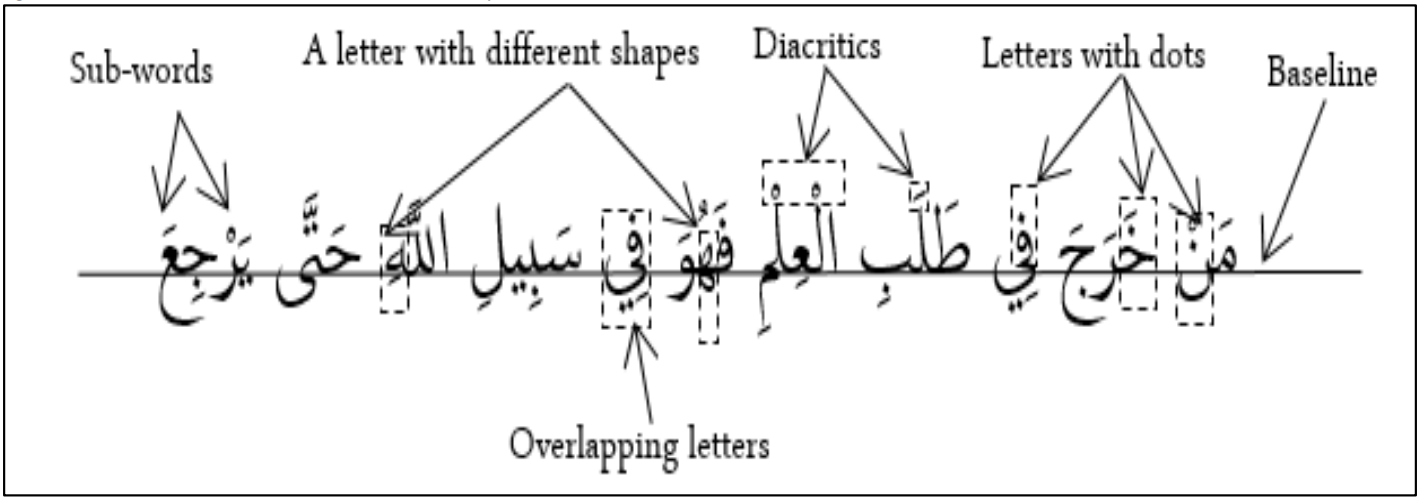
\includegraphics[width=13cm]{images/ocr2.png}
    \caption{Arabic script challenges characteristics.}
    \label{fig:ocr2}
\end{figure}


\textbf{The characteristics of Arabic script that may complicate recognition:}
    \begin{itemize}[itemsep=1pt, topsep=5pt]
        \item   Shapes and Positions.
        \item   Overlapping characters and Ligatures.
        \item   Diacritics.
        \item   Cursive.
        \item   Presence of dots.
    \end{itemize}  

\textbf{GENERAL ARABIC OCR METHODOLOGY (MODEL)}
\begin{figure}[H]
    \centering
    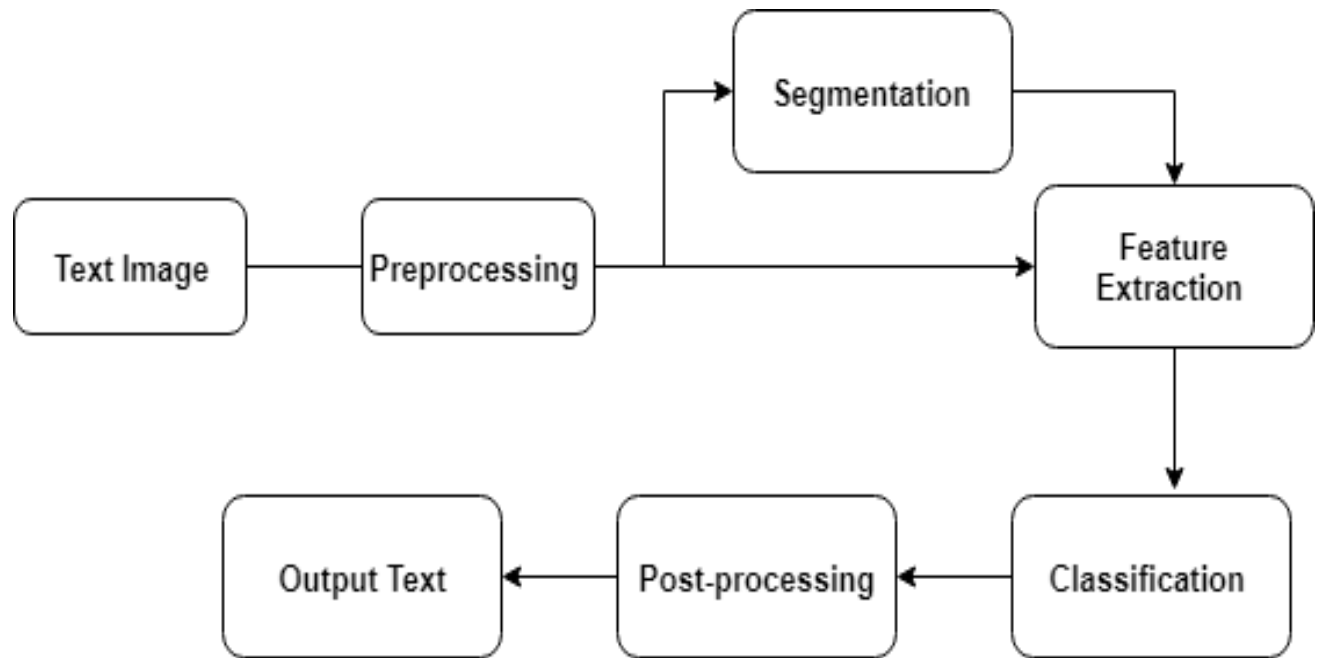
\includegraphics[width=11cm]{images/ocr3.png}
    \caption{General Arabic OCR methodology}
    \label{fig:ocr3}
\end{figure}

\begin{itemize}[labelindent=1em,labelsep=0.25cm,leftmargin=*]
        \item[\char `A)] \textbf{Preprocessing:- } 
        
        This is the first phase of \acrshort{ocr} methodology which is responsible for enhancing the readability of the input image.
Preprocessing is a combination of algorithms that are applied to the input image in order to reduce noise and alterations, thus simplifying the subsequent phases of \acrshort{ocr} methodology. There are various factors that affect the quality of the input image. A study lists the history of images, the printing process, the kind of font, the quality of paper, the condition of the image, and the image acquisition as the vital factors that influence the input image quality. 

Generally, several preprocessing operations are employed on the input image: binarization, layout analysis, thinning, smoothing and filtering, size and slant normalization, slant detection, skew detection, and baseline detection.

However, the selection of these operations, to be applied in the preprocessing, relies upon the conditions of the input image, such as the amount of noise and skew in the input image. 
the preprocessing techniques which are applied in Arabic \acrshort{ocr}:
\begin{itemize}[labelindent=1em,labelsep=0.25cm,leftmargin=*]
        \item[\char `1-] \textbf{Binarization:}\\
        Converting an input grayscale image into a binary image, in which a pixel has only two values 0 and 1
        \item[\char `2-] \textbf{Size Normalization:}\\
        Size normalization is commonly applied to characters or words by scaling the characters or the words to an adjusted size.
        This process is crucial for the recognition or classification phase.
        
       A study classified normalization methods into two approaches:
       \begin{itemize}[itemsep=1pt, topsep=5pt]
        \item[\char `-]  Moment-based Normalization.
        \item[\char `-]  Nonlinear Normalization 
        \end{itemize} 

        \item[\char `3-] \textbf{Remove Noise:}
        
        Noise may have a major impact on the performance of \acrshort{ocr} systems. several techniques have been introduced that are considered noise removal methods:
        \begin{itemize}[itemsep=1pt, topsep=5pt]
        \item[\char `-] Filtering: The median filter approach is commonly used in both printed text images and handwritten text images
        \item[\char `-] Morphological Operations (Smoothing)
            \begin{itemize}[itemsep=1pt, topsep=5pt]
            \item Dilation Algorithms, which are applied to broken letters.
            \item Erosion Algorithms, which are applied to text images with touching letters.
        \end{itemize} 
    \end{itemize} 
       
        \item[\char `4-] \textbf{Skew Detection and Correction:}
        
        Text image has zero rotation, yet when physically scanning the image manually, rotation of images up to 20 might occur. This rotation is called skew which results in non-zero skew text images.
        The skew can lead to incorrect recognition and baseline detection.
        It is impossible to segment a text if the text is rotated.
        The process of rotating the image with the purpose of correcting the skew is called skew correction. \\
        A study groups these methods into five groups:
        \begin{itemize}[itemsep=1pt, topsep=5pt]
        \item[\char `-] Projection Profile
        \item[\char `-] Hough Transform
        \item[\char `-] Fourier Transform
        \item[\char `-] Nearest Neighbor Clustering 
        \item[\char `-] Correlation
        \end{itemize} 

        \item[\char `5-] \textbf{Baseline Detection:}
        
        Arabic characters are joined through a horizontal line called the baseline.
        Graphically, the baseline can be described as the line which has the maximal amount of black pixels.
        This line contains critical information about the text, such as text orientation and the position of connection points between Arabic letters.
        The baseline detection techniques for Arabic script have been classified into four groups in 
        \begin{itemize}[itemsep=1pt, topsep=5pt]
            \item[\char `-] Namely
            \item[\char `-] Horizontal projection methods 
             \item[\char `-] Word skeleton method 
            \item[\char `-] Contour tracing and principal component analysis
        \end{itemize} 

         \item[\char `6-] \textbf{Thinning and Skeletonization:}\\
         The process of peeling off a pattern as many pixels as possible without affecting the general shape of the pattern In other words, it involves operations that can be implemented in order to produce the skeleton of text images. Thinning is a crucial processing step for text recognition. When applying thinning algorithms to Arabic scripts, various obstacles are encountered. One problem is the reduction in the number of dots in some Arabic characters as a result of the thinning process for which the number of dots is a crucial aspect in differentiating between these characters. Also, dots in Arabic characters are likely to be vulnerable to noise, results are shown in figure \ref{fig:thin}.

        \textbf{}
        \begin{figure}[H]
            \centering
            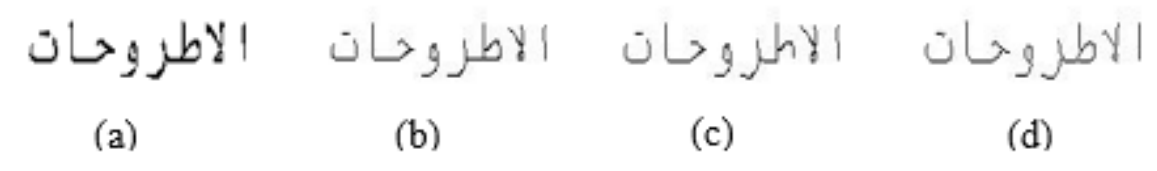
\includegraphics[width=10cm]{images/thin.png}
            \caption{Example results of different thinning algorithms: (a) original word, (b), (c), and (d) thinned word}
            \label{fig:thin}
        \end{figure}
    \end{itemize}

        \item[\char `B)] \textbf{Line Segmentation:-}
        
        During the segmentation phase, the text image is segmented into small components, with a page being segmented into lines, a line into words and a word into letters.
segmenting a text image can be graded into two types: 

\begin{itemize}[itemsep=1pt, topsep=5pt]
    \item \textbf{External Segmentation}:\\
    which refers to the document layout analysis, in particular page decomposition. Generally, it is relatively easy to segment a text line into words in printed text images, compared to handwritten text images which involve overlapping and touching characters by using vertical projection histogram profiles.

    \item \textbf{Internal Segmentation}:\\
    which deals with segmenting a word into characters. When reviewing segmentation methods in the literature, a major complication arises concerning the classification of word segmentation approaches.
\end{itemize} 

\clearpage

Arabic \acrshort{ocr} systems have been developed by two main paradigms: 
\begin{itemize}[itemsep=1pt, topsep=5pt]
    \item Holistic Approaches (segmentation–free) which require a large lexicon of Arabic words.
    \item Analytical Approaches (segmentation-based) where a word is segmented into units and each unit is recognized separately.
\end{itemize} 

\textbf{}
\begin{figure}[H]
    \centering
    
\includegraphics[width=9cm]{images/word.png}
    \caption{Segmenting Arabic lime into its words.}
    \label{fig:word}
\end{figure}

\textbf{}
\begin{figure}[H]
    \centering
    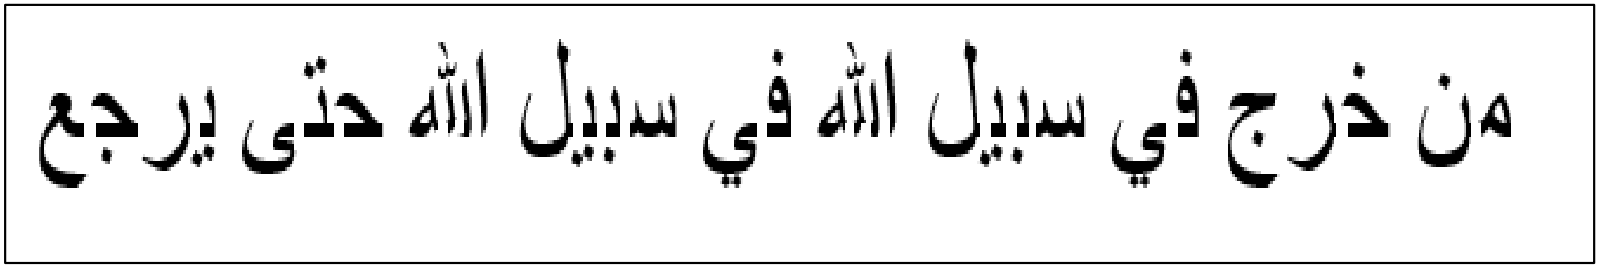
\includegraphics[width=9cm]{images/char.png}
    \caption{Segmenting Arabic words into their characters.}
    \label{fig:char}
\end{figure}

        \item[\char `C)] \textbf{Feature Extraction:-}\\
        The process of obtaining distinguishing attributes of the segmented character to be utilized by the next phase which is classification. The authors point out that the selection of feature extraction methods depends on the output of the preprocessing stage. The set of features extracted must match the specification of the selected classifier. However, the selection of feature types is a major issue in OCR development.

Such features can be categorized into three groups: 
\begin{itemize}[itemsep=1pt, topsep=5pt]
    \item \textbf{Structural Features}\\ Which illustrate a text image in terms of its topological and geometrical characteristics by using its local and global properties.

    \item \textbf{Statistical Features}\\ Which are derived from the statistical representation of patterns that provide a measurable event of interesting patterns. different approaches to produce statistical features. Some examples of the approaches are zoning, moments, characteristic loci, histograms, and crossing.

     \item \textbf{Global Transformation Features}\\ Which is applied to convert a skeleton or contour of a pattern by a linear transform into a form that reflects the most relevant features of the transformed pattern.
\end{itemize}

Finally, the feature extraction stage plays a critical role in Arabic  \acrshort{ocr} development in which distinguishing attributes are extracted and it is clear that each Arabic \acrshort{ocr} developer needs to apply different feature extraction approaches. Still, good features are required, which assist in distinguishing a character from other characters and maximize the accuracy performance simultaneously. Furthermore, these features must be selected specifically for a selected classifier. Some researchers apply different feature extraction methods in combination. However, this may cause extra complications in the implementation.

     
        
        \item[\char `D)] \textbf{Classification:-}
        
        The classification phase has the responsibility for assigning a pattern into a pre-classified class based on the features of the pattern which have been extracted in the previous phase. The pre-classified classes can be words, sub-words, characters or strokes, based on the OCR approach used. There are a number of different classification approaches that have been applied for Arabic  \acrshort{ocr}, such as Hidden Markov Models (HMM), Support Vector Machines ( \acrshort{svm}), K-nearest neighbour( \acrshort{knn}).
        
        \item[\char `E)] \textbf{Post Processing:-}
        
        Post-processing is the final stage of the development of Arabic \acrshort{ocr}. The objective of this step is to enhance the recognition accuracy by detecting and correcting linguistic misspellings in the produced \acrshort{ocr} text without human intervention Generally, post processing methods can be categorized into two main approaches: lexicon-based methods context-based (statistical) methods.

        The typical technique for correcting the mistakes of Arabic OCR outputs is the lexicon-based method which requires the utilization of an Arabic dictionary. This technique corrects errors without considering any contextual information in which the errors appear.

        \end{itemize}
        \acrshort{ocr} performance evaluation can be classified into two types:
        \begin{itemize}[itemsep=1pt, topsep=5pt]
            \item Black-box evaluation  
            \item White-box evaluation
        \end{itemize} 

        Performance evaluation of \acrshort{ocr} systems is essential for: monitoring the progress of \acrshort{ocr} systems development assessing the effectiveness of \acrshort{ocr} algorithms identifying open areas for further research providing scientific justification for the performance of \acrshort{ocr} systems.\\

For Arabic \acrshort{ocr}, conducting performance evaluation is challenging as no standard dataset is available. This accuracy metric is insufficient to assess how Arabic \acrshort{ocr} systems are overcoming the challenges of Arabic text. However, a study suggests a new set of objective performance metrics for evaluation Arabic \acrshort{ocr} with respect to the challenges of Arabic script which are character accuracy based on character position, dot character accuracy, zigzag-shaped character accuracy, loop-shaped character accuracy, and diacritics accuracy.

\subsection{Convolutional Neural Network (CNN)}
Convolutional Neural Networks (\acrshort{cnn}s) are very effective in perceiving the structure of handwritten characters/words in ways that help in the automatic extraction of distinct features and make \acrshort{cnn} the most suitable approach for solving handwriting recognition problems.\\

This paper \cite{CNN} proposes a method for recognizing the text from manuscript images using Convolutional Neural Networks (\acrshort{cnn}s). This includes preprocessing of the manuscript’s image, segmentation of the lines and characters in the manuscript, building a dataset that contains images for each character in different shapes, and classification of each character using \acrshort{cnn}.
Figure \ref{fig:CNN} shows the flow diagram of the methodology.

\begin{figure}[!htb]
    \centering
    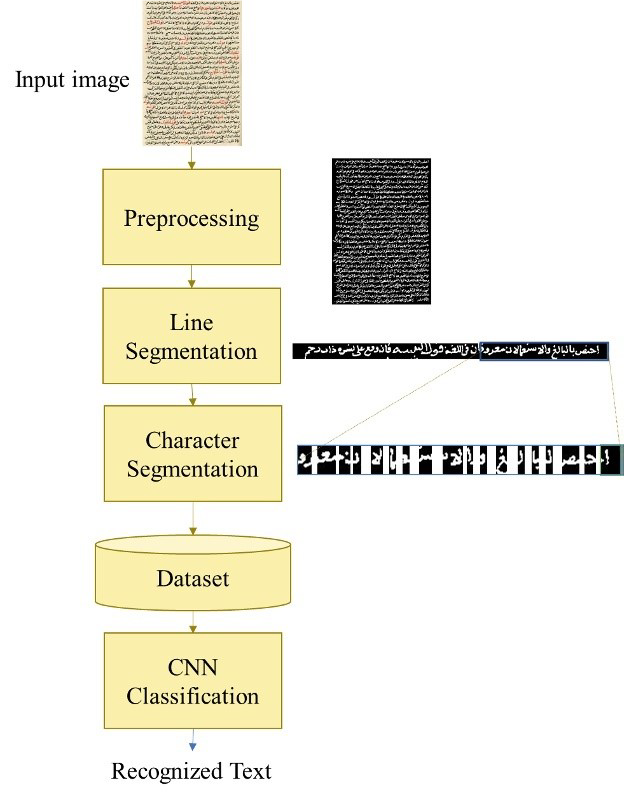
\includegraphics[width=8cm, height=8cm]{images/CNN.png}
    \caption{The flow diagram of the methodology.}
    \label{fig:CNN}
\end{figure}

\newpage

\begin{itemize}[labelindent=1em,labelsep=0.25cm,leftmargin=*]
        \item[\char `A)] \textbf{Preprocessing:-}
        
        The image is transformed into a binary representation. Figure \ref{fig:pre_cnn} illustrates the preprocessing stages.
        
        \begin{figure}[!htb]
            \centering
            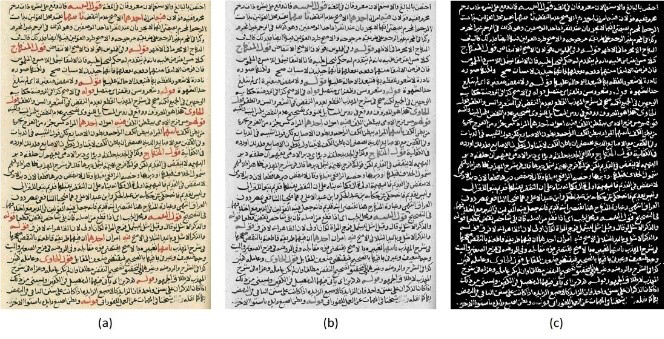
\includegraphics[width=10cm]{images/pre_cnn.png}
            \caption{(a) Original image. (b) Grayscale image. (c) Binary image.}
            \label{fig:pre_cnn}
        \end{figure}
        
        \item[\char `B)] \textbf{Line Segmentation:-} 
        
        Line segmentation is achieved via horizontal Projection Profile (\acrshort{pp}) for the image. Horizontal \acrshort{pp} is a method used to convert the image from 2D to 1D by calculating the densities \cite{PP}. They used this method to crop out each line at the points of lower density figure \ref{fig:line_cnn} shows the horizontal PP for the whole page, which is used to cut out each line.
        
        \item[\char `C)] \textbf{Character Segmentation:-} 
        
        Character segmentation is performed using vertical \acrshort{pp}. Vertical \acrshort{pp} is the same as horizontal \acrshort{pp}, but the direction of computing densities is different. In horizontal \acrshort{pp}, they calculate the densities for each row. However, in vertical \acrshort{pp} the calculation of densities is done for each column. Then, this method is used to cut each character in the line at lower densities of the horizontal \acrshort{pp}. Figure \ref{fig:char_cnn} shows how vertical \acrshort{pp} is used to  separate characters of each line in a sentence.
        
        \item[\char `D)] \textbf{Dataset:-}
        
        They have created three datasets in order to evaluate the classifier. These datasets contain images of Arabic letters in different states.
        
        \begin{enumerate}
        \item {\textbf{First Dataset:}}
        
        The first dataset has all 28 Arabic letters with an average of 40 images per letter. The total number of images is 2240 images.
        \item {\textbf{Second Dataset:}}
        
        The second dataset has partial letters from the first one. It includes 10 letters. However, we increase the number of images per letter. On average, there are 100 images per letter.
        \item {\textbf{Third Dataset:}} 
        
        The third dataset has the same letters presented in the second dataset with an average of 200 images per letter.
        \end{enumerate}
        The data within dataset is randomly divided into a training dataset and validation dataset. 85\% of the data is used for training and 15\% of the data is used for validation. This division is applied to each one of the three created datasets.

        \begin{figure}[!htb]
            \centering
            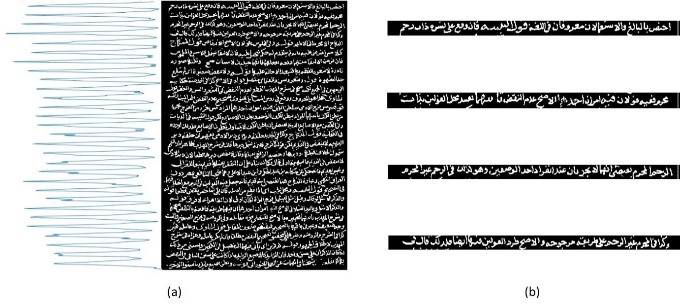
\includegraphics[width=10cm]{images/line_cnn.png}
            \caption{(a) Horizontal Projection Profile for the whole page image. (b) The segmentation of the first four lines.}
            \label{fig:line_cnn}
        \end{figure}
        
        \begin{figure}[!htb]
            \centering
            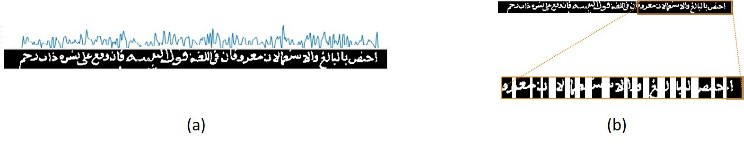
\includegraphics[width=10cm]{images/char_cnn.png}
            \caption{(a) : Vertical \acrshort{pp} for a line. (b) : Character segmentation for the first characters in the line.}
            \label{fig:char_cnn}
        \end{figure}
        
        
        \item[\char `E)] \textbf{\acrshort{cnn} Classification:-}
        
        Convolutional Neural Networks (\acrshort{cnn}s) are feedforward networks. In particular, the data flows within \acrshort{cnn} in one direction only. In general, \acrshort{cnn} consists of one or more convolutional and pooling layers followed by one or more fully connected layers. Figure \ref{fig:cnn_leyar} shows the general \acrshort{cnn} architecture for an image classification task.
        
        they defined the \acrshort{cnn} architecture for Arabic characters images classification as follow:
        \begin{enumerate}
        \item {\textbf{Input Layer:}}\\
       The input is an image that represents a single character from the historical Arabic manuscripts. They specify the image size to be 30-by-30-by-1 for all input images. The height and the width for the input image is equal to 30 pixels. As their images are grayscale images, the channel size is 1.
       
        \item {\textbf{Convolutional Layers:}}\\
        The convolution operation is a mathematical The convolution operation is a mathematical operation that takes an image along with a filter of a specific dimension, mostly an odd number, and applies this filter along with the image. An example of convolution is shown in figure \ref{fig:cnn-onvolution}. \\
        
        There are three convolutional layers. Each layer is followed by a
        nonlinear activation function, which is ReLU. The number of neurons varies in each convolutional layer. Particularly, the first layer has 8 neurons, the second layer has 16 neurons, and the third layer has 32 neurons.
        
        \begin{figure}[!htb]
        \centering
        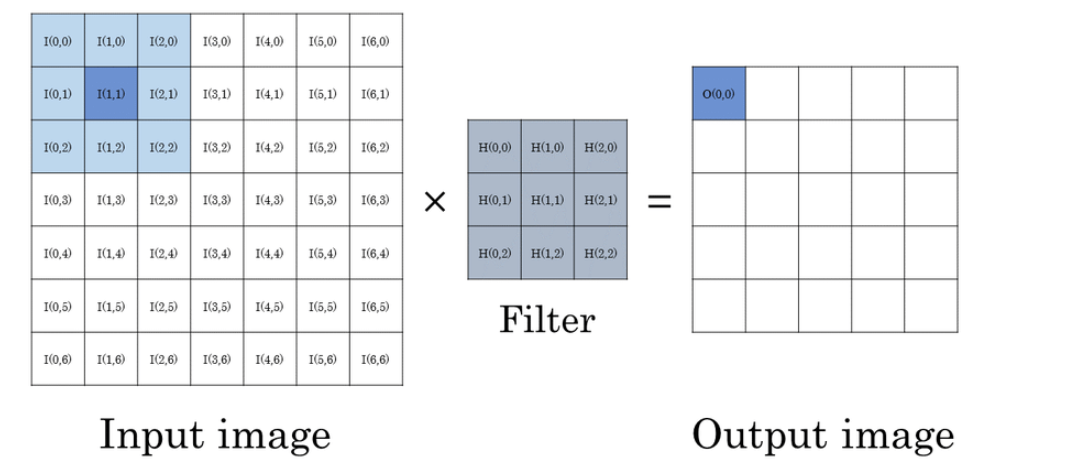
\includegraphics[width=8cm]{images/cnn-convolution.png}
        \caption{Example for convolution operation with the filter of size 3x3}
        \label{fig:cnn-onvolution}
        \end{figure}
        
        \item {\textbf{Max Pooling Layers:}} \\
Each convolutional layer is
followed by a down-sampling operation that reduces the
spatial resolution of the feature map. One way of downsampling
is to use max pooling, which returns the maximum
values of rectangular fields of inputs. The two arguments that
specify max pooling operation are pool size and step size.
Pool size is the size of the rectangular field of the input. Step
size specifies the size that the training function takes as it
scans along with the input. they made both pool size and step size
to equal 2.

        \item {\textbf{Fully Connected Layer:}}\\
In this layer, the neurons
connect to all neurons in the previous layer in order to
combine all features learned by the previous layers to identify
class label. Therefore, the number of neurons in this layer is
equal to the number of classes in the target dataset.

        \item {\textbf{Output Layer:}}\\
This layer uses the probabilities
returned by the Softmax activation function for each input
and assign the input to one of the output classes.
        \end{enumerate}
        
        \begin{figure}[!htb]
        \centering
        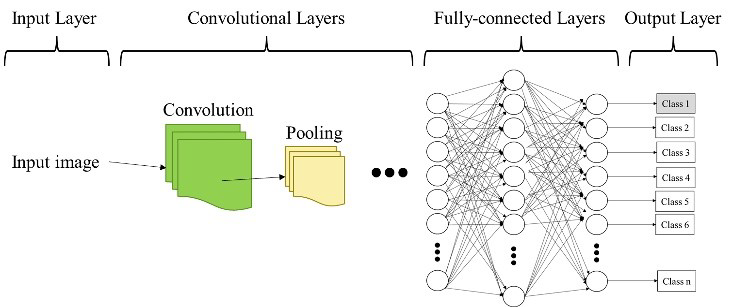
\includegraphics[width=10cm]{images/cnn_leyar.png}
        \caption{The general CNN architecture for an image classification task.}
        \label{fig:cnn_leyar}
        \end{figure}
        
    \end{itemize}
They applied \acrshort{cnn} classification to the three datasets and
compute the accuracy resulting from applying \acrshort{cnn} on each
dataset. Dataset1, which contains 56 classes with 40 images
per class, gives an accuracy of 74.29\%. On the other hand,
Dataset2 and Dataset3 give higher accuracies: 84.67\% and
88.20\%, respectively.

\section{Datasets}
Finding the appropriate and balanced data on which to work on and train the model is critical to the success of the experiments that take place during the work, so it was necessary to find a dataset that has a high degree of accuracy and also a large number of words that the model trains on. The stage of searching for a suitable dataset was very difficult so we decided to study all the available datasets that we found during the survey process. \\

Here, we reviewed some of the datasets as well studying each part, showing the advantages and disadvantages of each, choosing the most suitable dataset for us and mention its features in detail.

\subsection{Arabic Handwritten Character Dataset (AHCD)}
An open-source database of 16,800 characters was written by 60 participants; Their ages range from 19 to 40 years. It was used in more than one scientific paper concerned with recognizing handwritten Arabic words so that the accuracy of working with the \acrshort{cnn} model reached 97\% sometimes.\cite{altwaijry2021arabic} It is characterized by the diversity of fonts in it, but it was not suitable for the work we want because it is included in the intelligent systems that are interested in recognizing the handwritten Arabic language using the pen and modern writing tools. 

Not suitable because the way we decided to work on this project depends mainly on words and not characters. Figure \ref{fig:AHCD sample}

\begin{figure}[!htb]
    \centering
    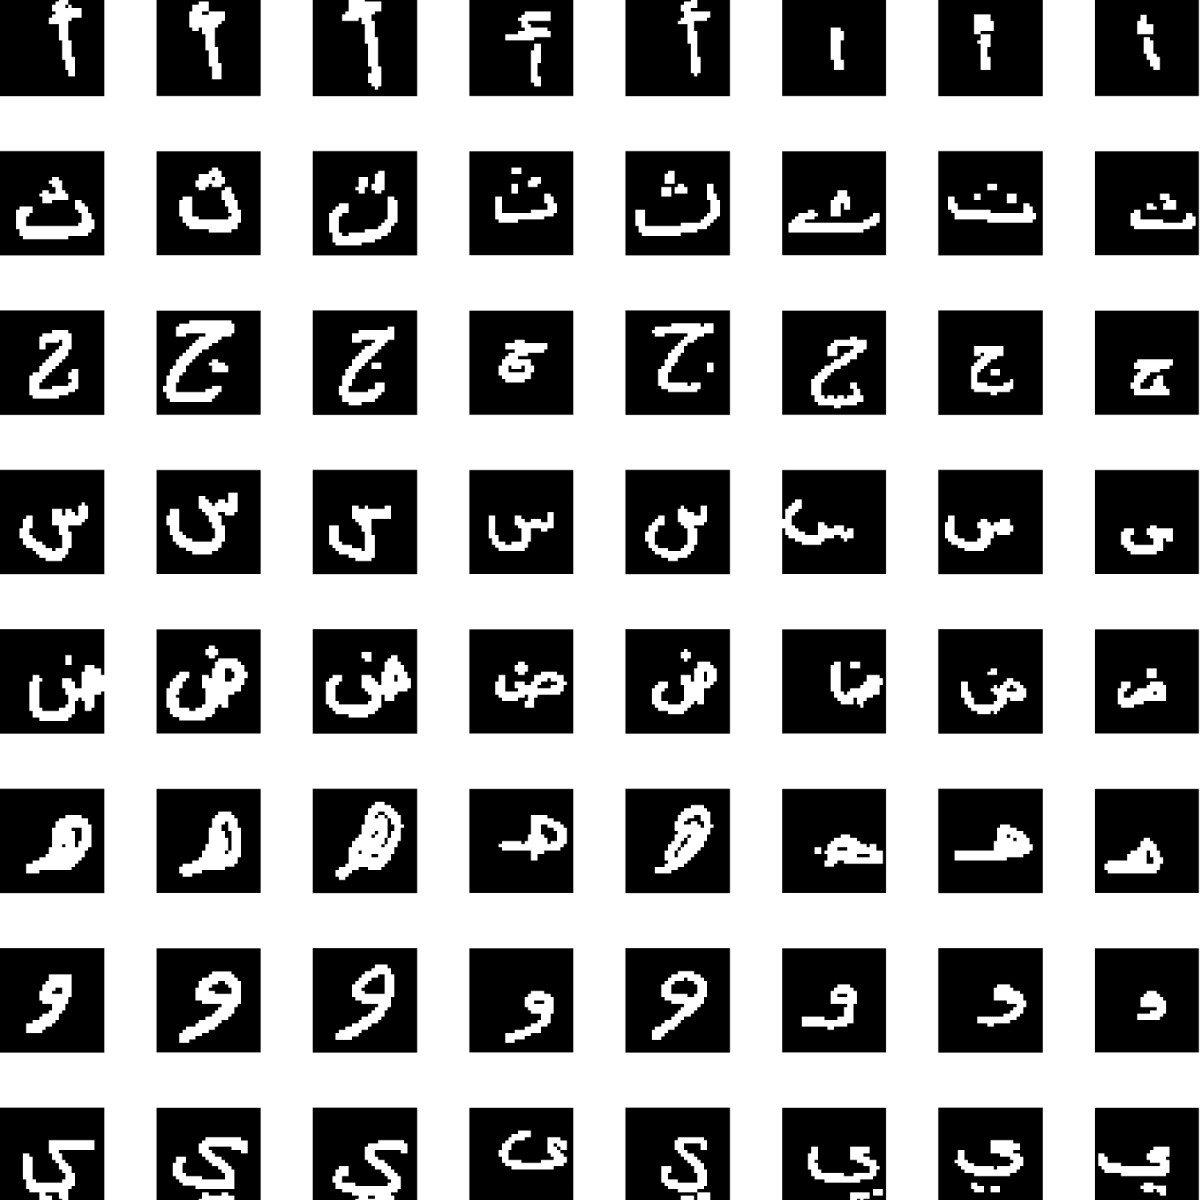
\includegraphics[width=7cm]{images/AHCD sample.png}
    \caption{Example from the AHCD dataset}
    \label{fig:AHCD sample}
\end{figure}

\subsection{Hijjaa Dataset}
The open-source database is written exclusively by children between the ages of 7 and 12. This dataset contains 47,434 characters written by 591 participants. It was used in one scientific paper we saw during the survey phase on the recognition of handwritten Arabic words until the accuracy of working with the \acrshort{cnn} model reached 88\%.\cite{altwaijry2021arabic} But it is also written with modern tools such as the pen and was written by the hands of young children and is also divided into letters, and as we mentioned it does not fit the method of work we have chosen. You can download the dataset from \url{https://github.com/israksu/Hijja2}

\subsection{KHATT Dataset}
KHATT dataset \cite{KHATT} is a constructed dataset consisting of images containing Arabic text collected from the web along with their ground truth.
A portion of the text includes Arabic diacritics. and Multiple Arabic fonts that closely resemble the old fonts used in historical manuscripts (dating back to the 18th century) are used. We show an example in figure \ref{fig:Sample-text-images-from-the-KHATT-dataset}

There are four categories of images:

\begin{itemize}[itemsep=1pt, topsep=5pt]
    \item Full sequences (images with more than five words).
    \item Short sequences (images that have five or fewer words).
    \item With diacritics (images with more than five words with diacritics).
    \item Short sequences with diacritics (images with five or fewer words, with diacritics).
\end{itemize}  

\noindent
The handwritten manuscripts from the KHATT database are also included (KHATT contains unconstrained handwritten Arabic Texts written by 1000 different writers).\cite{mostafa2021ocformer}

\begin{figure}[!htb]
    \centering
    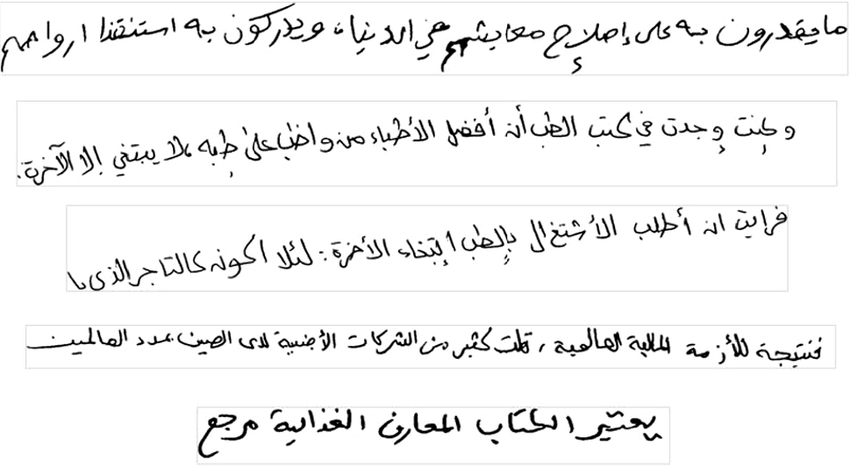
\includegraphics[width=10cm]{images/Sample-text-images-from-the-KHATT-database.PNG}
    \caption{Example from the KHATT dataset}
    \label{fig:Sample-text-images-from-the-KHATT-dataset}
\end{figure}


\subsection{IFN/ENIT Dataset}
The IFN/ENIT \cite{IFNENIT} database contains training and testing materials for Arabic handwriting recognition software. There are more than 2,200 binary images of sample figures in handwriting from 411 writers\cite{ali2019efficient}, but they are not suitable for work in manuscripts due to the different tools of the book and are not similar to the nature of Arabic manuscripts and their number is also very small in relation to other datasets. We show an example of them in the figure \ref{fig:Sample text images from the IFN/ENIT dataset}

\begin{figure}[!htb]
    \centering
    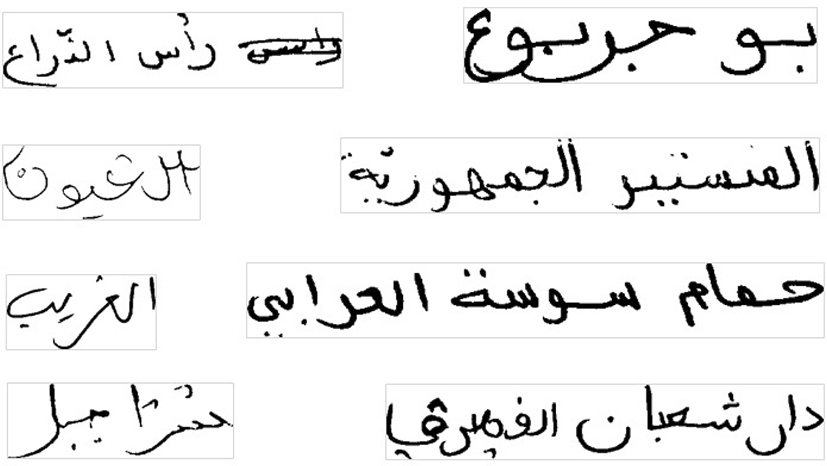
\includegraphics[width=8cm]{images/Sample-text-images-from-the-IFN-ENIT-database.png}
    \caption{Sample text images from the IFN/ENIT dataset}
    \label{fig:Sample text images from the IFN/ENIT dataset}
\end{figure}

\subsection{RASAM (Maghrebi) Dataset}
In the paper \cite{RASAM} present a Maghrebi dataset, This Dataset is made up of 300 annotated images, with their related ground truth stored in an XML file (page XML format). Images come from three manuscripts selected among the collections of the Bibliotheque Universitaires des LAngues et Civilisations (BULAC): two manuscripts belong to the historical genre (MS.ARA.1977 and MS.AR.417) and the third one has to do with inheritance law (MS.ARA.609). An example of RASAM dataset is shown in the figure \ref{fig:RASAM sample dataset}. The images of the dataset are in JPEG format and have varying resolutions from 96 DPI to 400 DPI.

\begin{figure}[!htb]
    \centering
    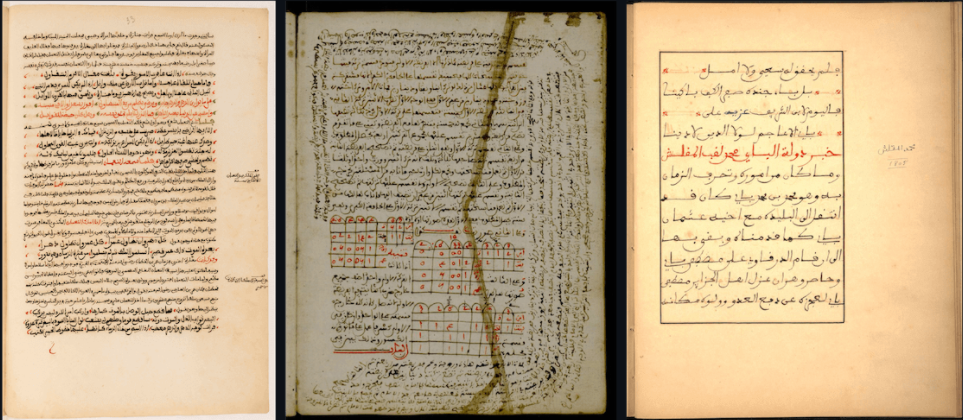
\includegraphics[width=12cm , height=7cm]{images/RASAM sample.png}
    \caption{Sample text images from the RASAM dataset}
    \label{fig:RASAM sample dataset}
\end{figure}

\subsection{IBN SINA Dataset}
It is a dataset that has been published and is taken from a philosophical book by Ibn Sina, Allows images in binary and color formats, The dataset consists of 51 folios which correspond to 20722 CCs (almost 500 CC on each folio)\cite{farrahi2010ibn}.
This dataset has been used in many scientific papers that we have seen in the survey phase and has had very good results, especially when it is used in a CNN-GRU model\cite{hassen2021subword}.
This set of data has many features such as it is large in proportion to the training of the model, and also the images are in color and gray, but they are from one book and in one font and indicate the shape of the letters in a specific time period, and it does not have the diversity required in our project to identify the largest number of manuscripts.

\begin{figure}[!htb]
    \centering
    \begin{minipage}{0.45\linewidth}
        \centering
        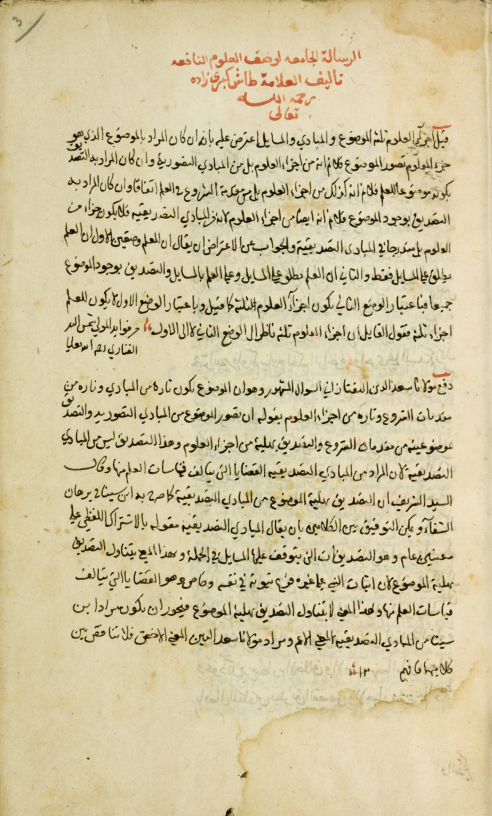
\includegraphics[width=0.6\linewidth, height=0.8\linewidth]{images/IBN SINA original image.png} % first figure itself
        \caption{Original image in IBN SINA}
        \label{fig:adaptive-gaussian}
    \end{minipage}\hfill
    \begin{minipage}{0.45\linewidth}
        \centering
        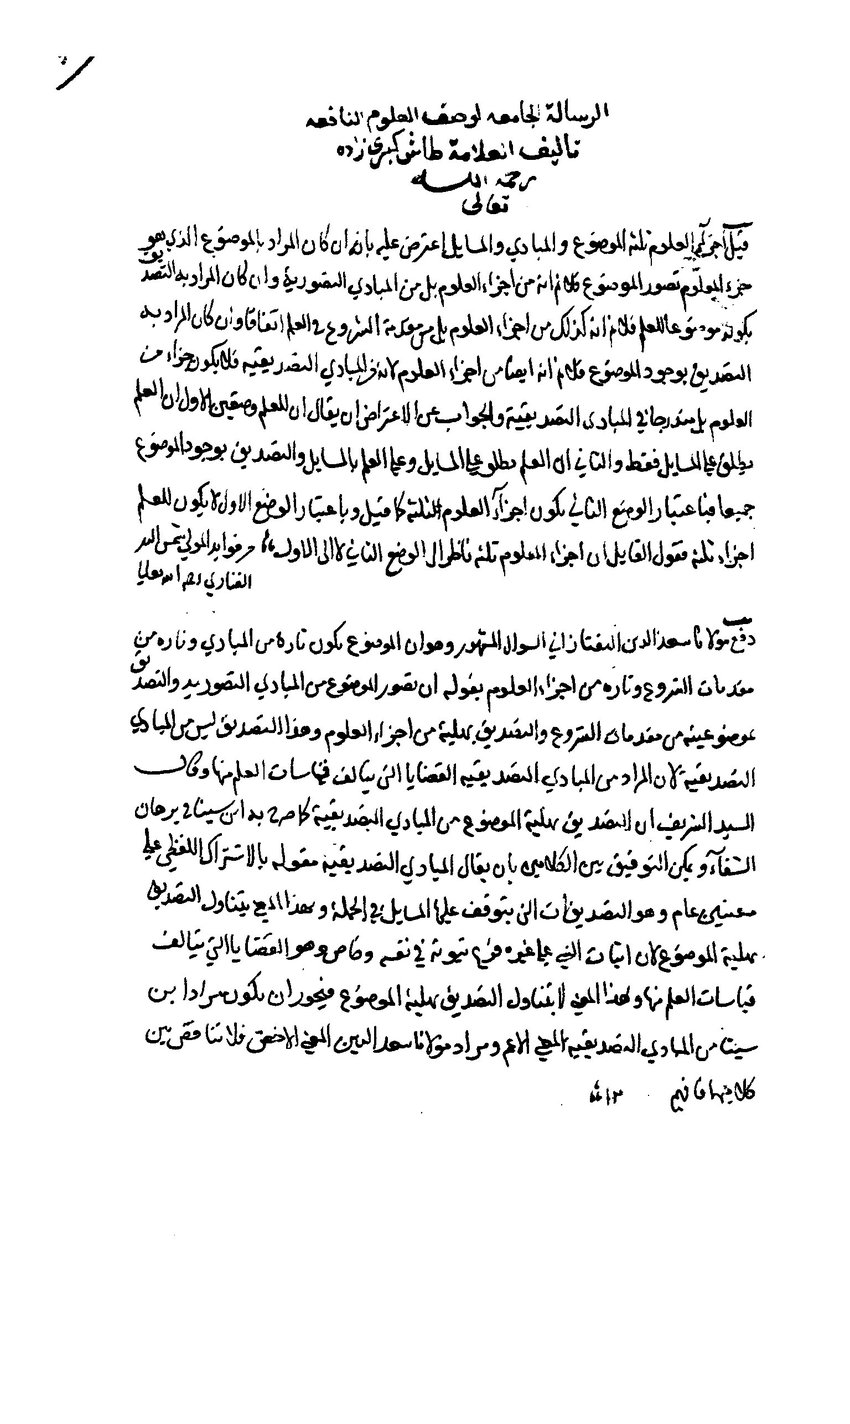
\includegraphics[width=0.6\linewidth, height=0.8\linewidth]{images/IBN_SINA binarized sample.png} % second figure itself
        \caption{Binarized image in IBN SINA}
        \label{fig:IBN_SINA binarized sample}
    \end{minipage}
\end{figure}


\subsection{VML-HD Dataset}
In the paper \cite{VMLHD} present a new database with a handwritten Arabic script. This dataset is based on five books written by different authors in the years 1088 - 1451 figure \ref{fig:VML-HD sample dataset}, and the entire 668 pages are annotated at the sub-word level. For each page, we manually applied bounding boxes to the different subwords and annotated the character sequences. It consists of 159,149 subwords of 326,289 letters of a vocabulary of 5509 forms of subwords. \\
One of the advantages of this data set is that it contains examples of 5 books of different formats and character shapes, and they indicate five different eras in Arab Islamic history. \\

\begin{figure}[!htb]
    \centering
    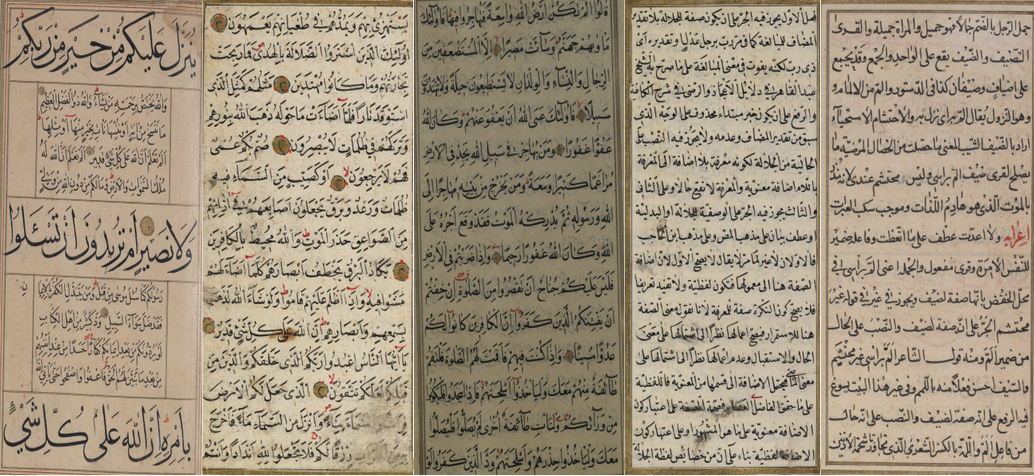
\includegraphics[width=13cm]{images/vml-hd-sample.PNG}
    \caption{Sample text images from the five books that make up the VML-HD dataset}
    \label{fig:VML-HD sample dataset}
\end{figure}


It was created by a team from one of the universities in the Middle East and they made a great effort, they used in this work a WebGT ground truth system\cite{biller2013webgt}, which is a web-based system for ground truth generation and provides a user-friendly interface for quick annotation of degraded documents in general, and historical document images in particular. Using this system they marked the bounding of the sub-words found on each page. They manually applied each bounding box around the sub-words present in the image, then they annotated each bounding box with its corresponding sequence of characters. they have marked, in total, 121,636 sub-words of 1,731 different forms of sub-words\cite{VMLHD}. \\

\noindent
The WebGT website exports an XML file in Hadara\cite{pantke2013hadara} format. Each book has its own Hadara XML file which contains the coordinates of all the bounding boxes of all the images annotated in that book, as well as the sequence of characters for each bounding box applied in Arabic text. They also generated a Hadara XML file for each page in addition to the file for each book. This file contains the coordinates of the bounding boxes and the sequence of the characters for the specific page only. \\

\begin{figure}[!htb]
    \centering
    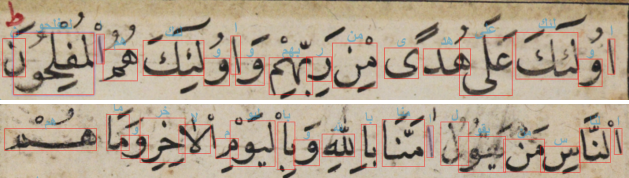
\includegraphics[width=10cm, height=3cm]{images/Web-GT.png}
    \caption{An example of an annotated line done using Web-GT framework.}
    \label{fig:Web-GT.png}
\end{figure}

Finally, they generated the ground truth data for each sub-word found in the dataset. The ground truth data consists of the following fields: Book number, Page number, Sub-word id, Location coordinates, Arabic annotation, Latin annotation, and Sub-word length. Two examples of the ground truth gathered for sub-words can be seen in Table \ref{table:2.1}.

\begin{table}[!htb]
\begin{center}
\begin{tabular}[htbp!]{ | c | m{3cm}| m{3cm} | } 
  \hline
  Image & 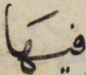
\includegraphics[width=1.5cm ]{images/feha.png} & 
\includegraphics[width=1.5cm ]{images/khla.png} \\ 
  \hline
  Book number & 3158466 & 187370 \\ 
  \hline
  Page number & 006-2 & 0013-2 \\ 
  \hline
  Segment Id & 183380 & 187370 \\ 
  \hline
  Location coordinates & y=1249 x=856  y=1249 x=945  y=1352 x=945
 y=1352   x=856 & y=1212 x=649  y=1212 x=722  y=1306 x=722  y=1306  x=649 \\ 
   \hline
  Arabic annotation & \<فيها>\ &\<خلا> \\ 
  \hline
\end{tabular}
\end{center}
\caption{Two examples of ground truth information in the VML-HD dataset}
\label{table:2.1}
\end{table}

\newpage

\section{Image Preprocessing}
In this section, we will be discussing our experiments performing preprocessing on images shown in figure \ref{fig:preprocessing} . we have used Python language, Which includes using different libraries. The main ones are OpenCV and scikit-image.

\begin{figure}[!htb]
    \centering
    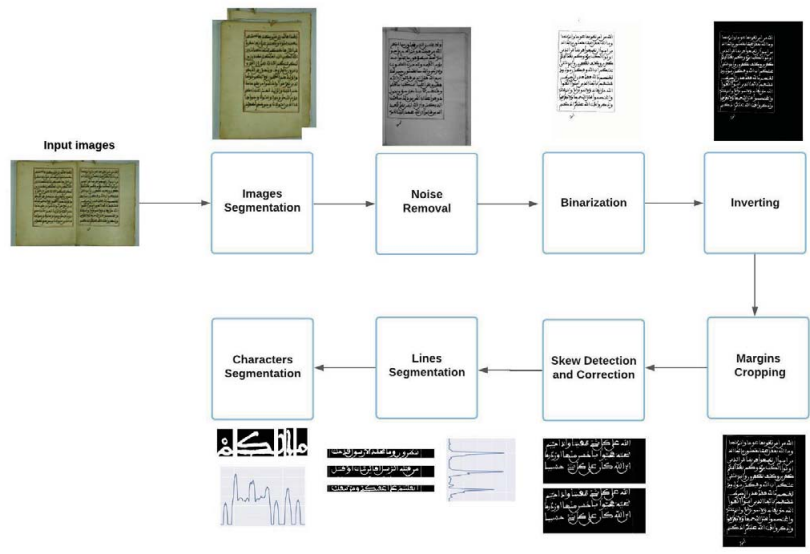
\includegraphics[width=14cm]{images/preprocessing.png}
    \caption{Preprocessing steps for segmentation}
    \label{fig:preprocessing}
\end{figure}

\begin{itemize}[labelindent=1em,labelsep=0.25cm,leftmargin=*]
        \item[\char `A)] \textbf{Noise Removal:-}
       
        In paper, \cite{Shams2020} This step focuses on removing any noise from the images
        which contain the text to be segmented. 
        Since the manuscript is ancient and written more than 250
        years ago, pages contain a considerable amount of noise.
        Furthermore, an important characteristic of the Arabic language is
        diacritics which can be added to letters in different locations,
        e.g., at the top or the bottom of the letter. These diacritics make
        the text segmentation process more complicated. As a solution
        to this, colored images of the manuscripts were split into three
        main channels: R, G, and B. After that, the R channel was
        chosen as it was the clearest one among them.
        Another step of noise removal that was taken is applying
        Gaussian filter is in charge of smoothing the image.
        \item[\char `B)] \textbf{Binarization and Inverting:-}
        
        This step aims to convert the colored images into binary
        images where the text (foreground) is in white and the background is in black. This is required in the PP method.
        Firstly, the images are converted into grayscale. Secondly,
        images are converted into binary by applying a specific
        thresholding technique. For this reason, different methods were
        applied to a sample of the manuscript in order to achieve the
        best results. There are two main types of thresholding methods: global and local. Global methods choose one threshold value for the whole image. On the other hand, local methods choose
        a different threshold value for each pixel by calculating the
        features of its neighbors. Firstly, two local methods were
        applied which are adaptive Gaussian thresholding in 
        figure \ref{fig:adaptive-gaussian} and adaptive mean thresholding in figure \ref{fig:adaptive-mean} 
        
        \begin{figure}[!htb]
            \centering
            \begin{minipage}{0.45\linewidth}
                \centering
                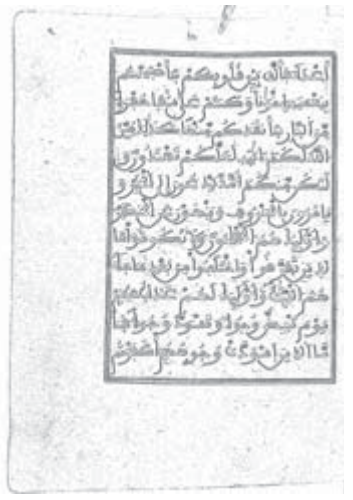
\includegraphics[width=0.7\linewidth, height=0.9\linewidth]{images/adaptive-gaussian.png} % first figure itself
                \caption{Adaptive Gaussian}
                \label{fig:adaptive-gaussian}
            \end{minipage}\hfill
            \begin{minipage}{0.45\linewidth}
                \centering
                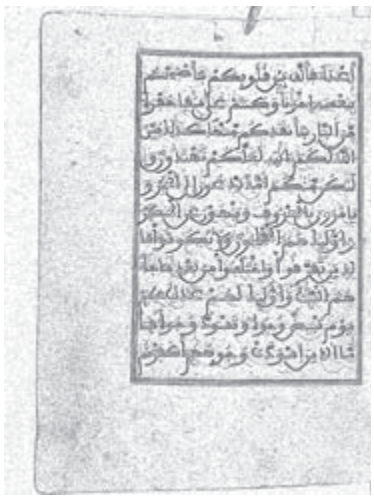
\includegraphics[width=0.7\linewidth, height=0.9\linewidth]{images/adaptive-mean.png} % second figure itself
                \caption{Adaptive Mean}
                \label{fig:adaptive-mean}
            \end{minipage}
        \end{figure}
        
        It is clear that both results are considered poor. So, other global methods were applied such as mean in figure \ref{fig:thresholding} a, Otsu in figure \ref{fig:thresholding} b, and
        minimum in figure \ref{fig:thresholding} c. It is clear that the minimum method gives out
        the best result so it was the chosen method for binarization.
        
        \begin{figure}[!htb]
            \centering
            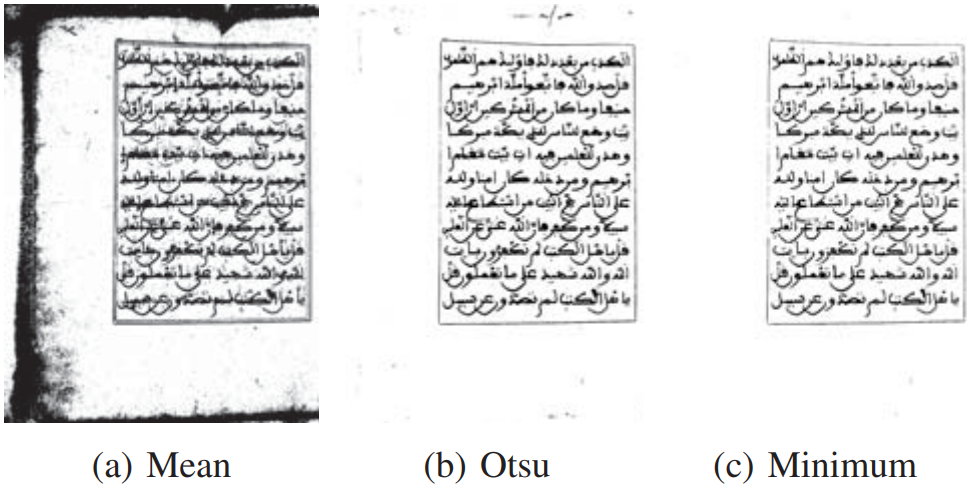
\includegraphics[width=10cm]{images/thresholding.png}
            \caption{Global thresholding methods results}
            \label{fig:thresholding}
        \end{figure}
        
        After applying the binarization, the result was the text
        (foreground) in black color and the background in white color.
        In order to make the text become more clear, the inverting step
        was performed where the text (foreground) has become in
        white color and the background in black color.
        
        \item[\char `C)] \textbf{Margins Cropping:-}
        
        Each page in the original manuscript contains margins in
        three directions depending on the side of the written text.
        Therefore, it was needed to crop these margins so that the
        images will contain only text without empty spaces.
        This process is composed of many steps. Firstly, inverted
        images are used as input, then the adaptive (local) threshold is
        calculated for each block, where the block size is set to 35 and
        the max value of the threshold is set to 255. After that, erosion
        method is applied to the image using a structural element of
        size 40×40. Then, a mask is extracted from the erosion image
        by applying a global thresholding with a value of 120. The next
        step is that the edges of the images are detected and the max and min values of both x and y axes are calculated. Finally,
        these values will be used to crop image’s margins.
       
        \item[\char `D)] \textbf{Skew Detection and Correction:-}
        
        Skew happens when the image is not set correctly on the
        scanner or the camera, which results in poor accuracy in the
        segmentation phase.
        Some parts of the manuscript contain skewed images which
        will therefore affect the segmentation phase. Therefore, a skew
        detection and correction method was applied where the binary
        image is used as input. Then, different values of angles are
        tested in order to find the best angle value. This is done by
        calculating the Horizontal PP. The difference between each
        value and the value next to it powered by two is calculated. If
        the image is skewed, the sum of the differences between these
        two values will be small. In contrast, if the image’s skew is
        set correctly, the difference between them will be large. To
        clarify this further, figure \ref{fig:skew} shows two Horizontal PP, where
        figure \ref{fig:skew}a is the correctly skewed page, and figure \ref{fig:skew}b is the same
        page but after rotating it by 30°. Finally, the angle that leads
        to the maximum score will be chosen. After that, the image
        will be rotated using this angle value.
        \begin{figure}[!htb]
            \centering
            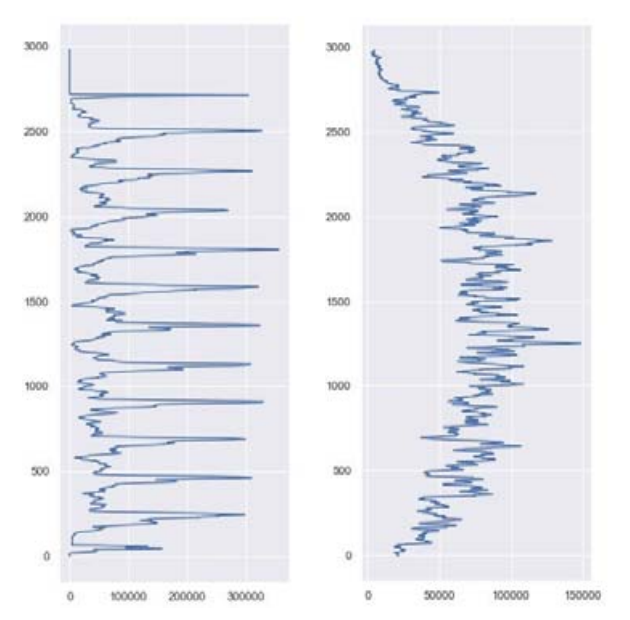
\includegraphics[width=5cm]{images/skew.png}
            \caption{The effect of skew on Horizontal PP}
            \label{fig:skew}
        \end{figure}
    \end{itemize}

\clearpage

\section{Line Segmentation}
Text-lines are hard to segment in the context of Arabic manuscripts, because of the narrowly spaced text lines with touching or overlapping components, the varying spaces between words, the ascendant or descendant letters, special marks, and dots, calligraphy, etc.\\

In this paper \cite{9257759} the
the proposed system is used  to automatically extract text lines from images of unconstrained handwritten Arabic texts. Each text line is detected by its baseline based on text-line masks which are predicted by a deep neural network called \acrshort{AR2U} based on the U-Net model with an Attention mechanism. The \acrshort{AR2U} model is used to allow a pixel-wise classification and therefore to separate text-lines pixels from the background one.
It tested on BADAM: A public dataset for baseline detection in Arabic script manuscripts that involves complex layouts as well as curved and arbitrarily oriented text-lines and overlaps between adjacent text-lines, words, or sub-words figure \ref{fig:example1}.\\ 

This model achieves the best performance with a Precision of 0.932\% which competes with current state-of-theart approaches.Figure \ref{fig:example2} shows an example of model prediction on an image
of the dataset.

\begin{figure}[H]
    \centering
    \begin{minipage}{0.50\linewidth}
        \centering
        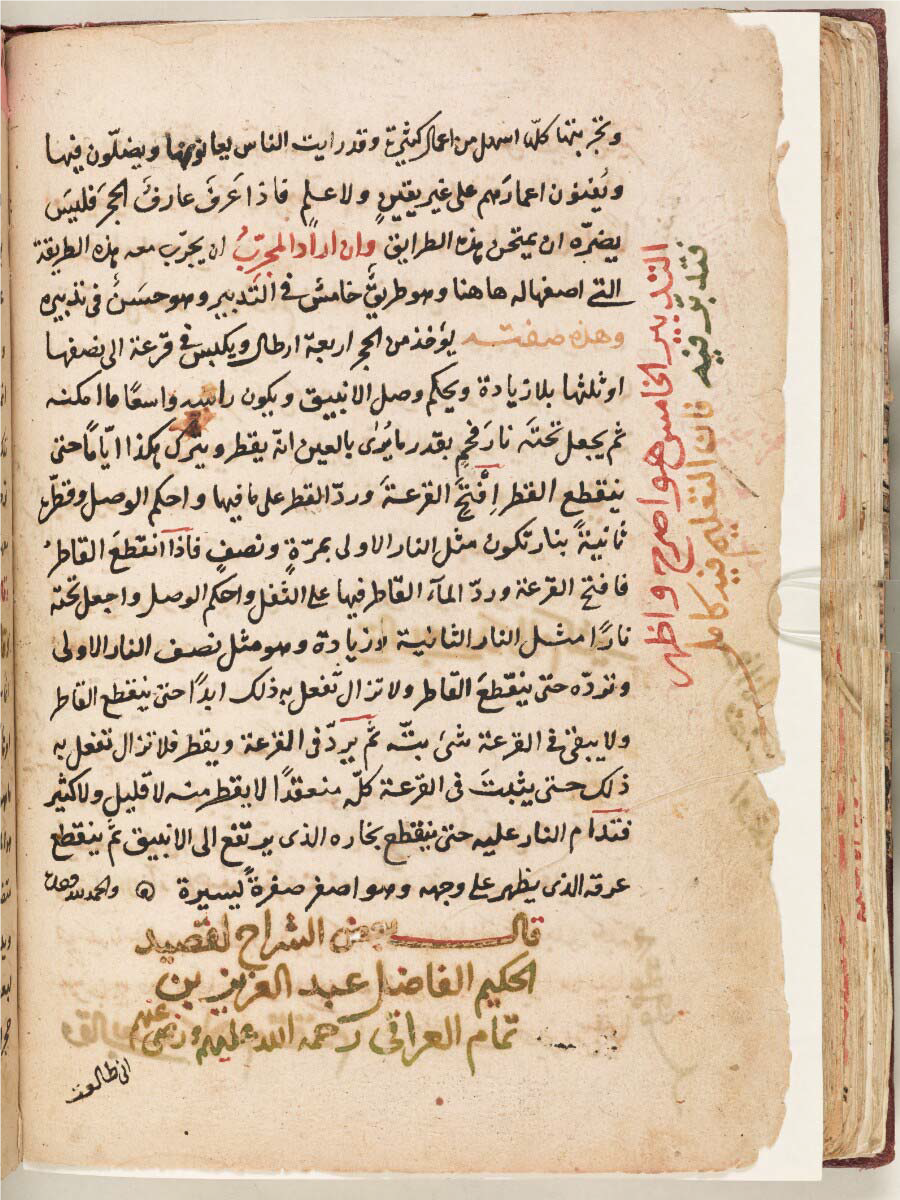
\includegraphics[width=0.7\linewidth, height=0.9\linewidth]{images/example.png} % first figure itself
        \caption{Example of used documents}
        \label{fig:example1}
    \end{minipage}\hfill
    \begin{minipage}{0.50\linewidth}
        \centering
        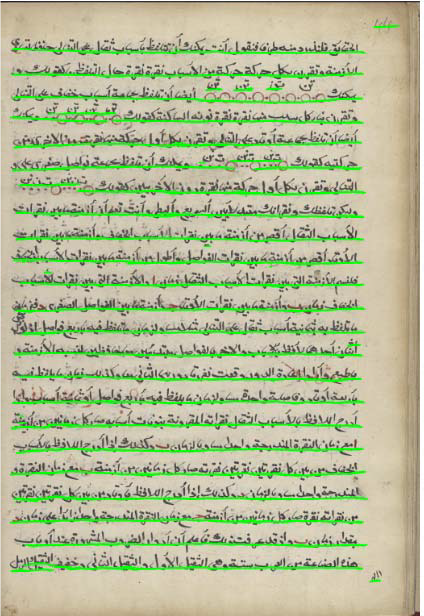
\includegraphics[width=0.7\linewidth, height=0.9\linewidth]{images/example2.png} % second figure itself
        \caption{Model predictions result}
        \label{fig:example2}
    \end{minipage}
\end{figure}

This paper \cite{8892920} proposed a novel approach to carry out the segmentation of Arabic manuscripts into text-lines and words, using deep learning. The proposed text-line segmentation system uses an \acrshort{RU} to extract x-heights from text images, then a post-processing step extracts baselines figure \ref{fig:X-height}. The word segmentation system uses a \acrshort{cnn} with a \acrshort{blstm}, then a \acrshort{ctc} to find the alignment between the text-line transcription and the text-line image.

\begin{figure}[!htb]
    \centering
    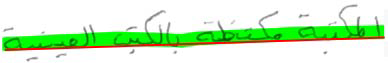
\includegraphics[width=10cm]{images/X-height.png}
    \caption{X-height (green) and baseline (red) of a text line.}
    \label{fig:X-height}
\end{figure}

\begin{itemize}[labelindent=1em,labelsep=0.25cm,leftmargin=*]
         \item[\char `A)] \textbf{Text Line Segmentation:-}
         
        For text-line segmentation, we extracted the x-heights of
        text-lines, by the use of a ground truth that separates the input images into three classes which shown in figure \ref{fig:result_of_line}(b):
        \begin{enumerate}
            \item Background
            \item Paragraphs
            \item Text-lines x-heights in each paragraph
        \end{enumerate}
        
        \begin{figure}[!htb]
            \centering
            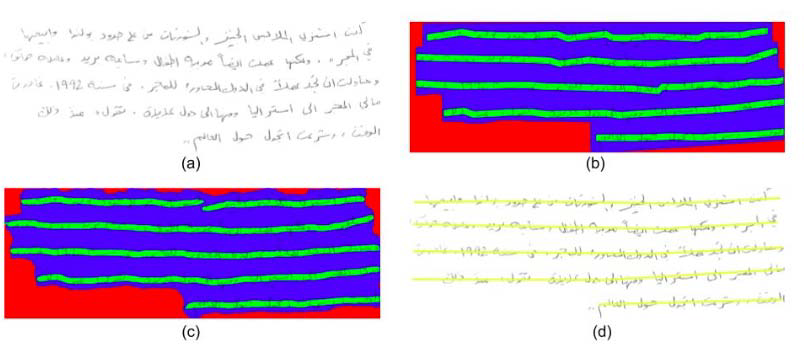
\includegraphics[width=9cm]{images/result_of_line.png}
            \caption{Results of text-line segmentation: a) the original image, b) the ground truth composed of three classes (background: red; paragraph: blue; x-height: green), c) the output of the RU-net, d) the final result after post-processing.}
            \label{fig:result_of_line}
        \end{figure}
        
        \item[\char `B)] \textbf{Word Segmentation:-}
        
        For word segmentation, firstly used a \acrshort{cnn} to extract the most important features from the text-line images. All images have a normalized size of 48×1600. Every convolutional block is followed by a batch normalization that greatly reduces the vanishing gradient problem and makes the use of dropout unnecessary. The output of the \acrshort{cnn} is then sequentially passed to a \acrshort{blstm} having 100 neurons for each LSTM and followed by a \acrshort{ctc} function, as shown in figure \ref{fig:seg_network}
        
        Their two classes: \textbf{word}(1) and \textbf{space}(2). The
        provided ground truth is the text-lines Unicode transcription
        where each word is labeled 1 and each space 0, as displayed in the figure \ref{fig:word_seg}. The \acrshort{ctc} decoder output is the found sequence workspace. After the training step, the projection of the probabilities of class space (output of the \acrshort{blstm}) is made on the image.
        \begin{figure}[!htb]
        \centering
        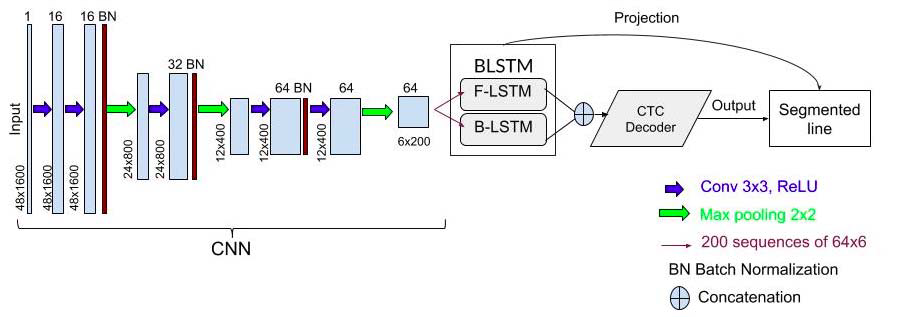
\includegraphics[width=10cm]{images/seg_network.png}
        \caption{Proposed word segmentation network.}
        \label{fig:seg_network}
        \end{figure}
        
        \begin{figure}[!htb]
        \centering
        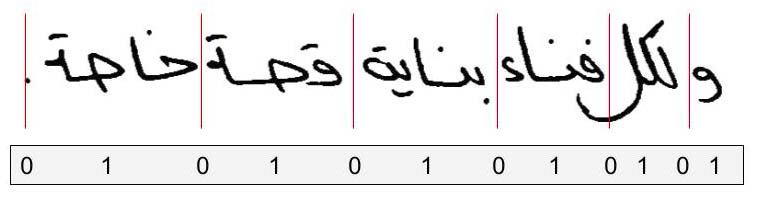
\includegraphics[width=8cm]{images/word_seg.png}
        \caption{Ground truth provided to the CTC (1: word; 0: space).}
        \label{fig:word_seg}
        \end{figure}
    The experimental results confirm a segmentation success rate of no less than 96.7\%. 
 \end{itemize}

This paper \cite{FCN} presents a method for text line segmentation
of challenging historical manuscript images. These manuscript images contain narrow interline spaces with touching components, interpenetrating vowel signs, and inconsistent font types and sizes. In addition, they contain curved, multi-skewed, and multi-directed side note lines figure \ref{fig:text line problems} within a complex page layout. Therefore, bounding polygon labeling would be very difficult and time consuming. Instead, they rely on line masks that connect the components on the same text line. Then these line masks are predicted using a Fully Convolutional Network (\acrshort{fcn}). \acrshort{fcn} has been successfully used for text line segmentation of regular handwritten document images. This paper shows that \acrshort{fcn} is useful with challenging manuscript images as well. Using a new evaluation metric that is sensitive to over segmentation as well as under segmentation.Tested on the new challenging handwritten document dataset. The model achieved 89\% training accuracy and 88\% validation accuracy on average.

\begin{figure}[!htb]
    \centering
    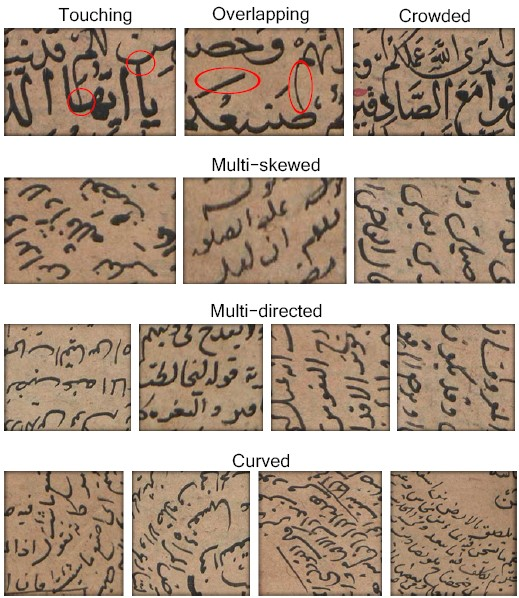
\includegraphics[width=7cm]{images/text line segmentation problems.jpg}
    \caption{Text line segmentation problems with challenging handwritten documents.}
    \label{fig:text line problems}
\end{figure}

\noindent
The following steps summarize paper's flow
\begin{enumerate}
  \item \acrshort{fcn} architecture figure \ref{fig:fcn_arc}.
  \item Pre-processing figure \ref{fig:fcn_image}.
  \item Training and testing.
  \item Post-processing figure \ref{fig:fcn_post}.
  \item Connectivity component based line extraction accuracy metric.
\end{enumerate}

\begin{figure}[!htb]
    \centering
    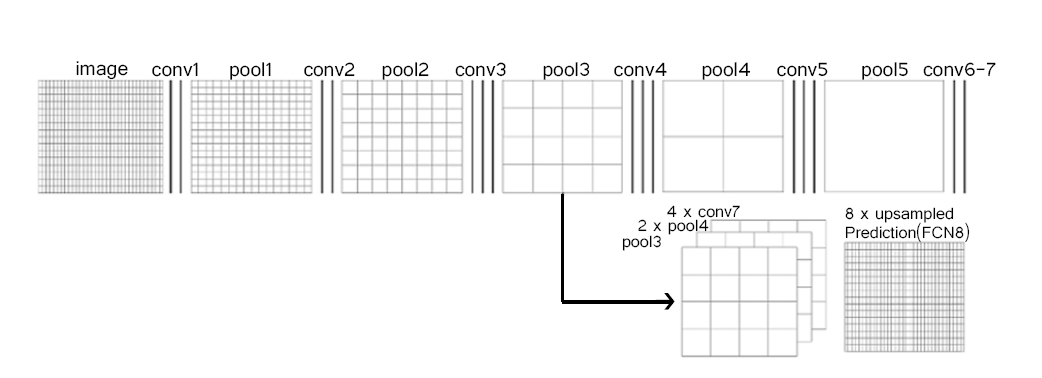
\includegraphics[width=15cm]{images/FCN_arc.png}
    \caption{The \acrshort{fcn} architecture}
    \label{fig:fcn_arc}
\end{figure}

\begin{figure}[!htb]
    \centering
    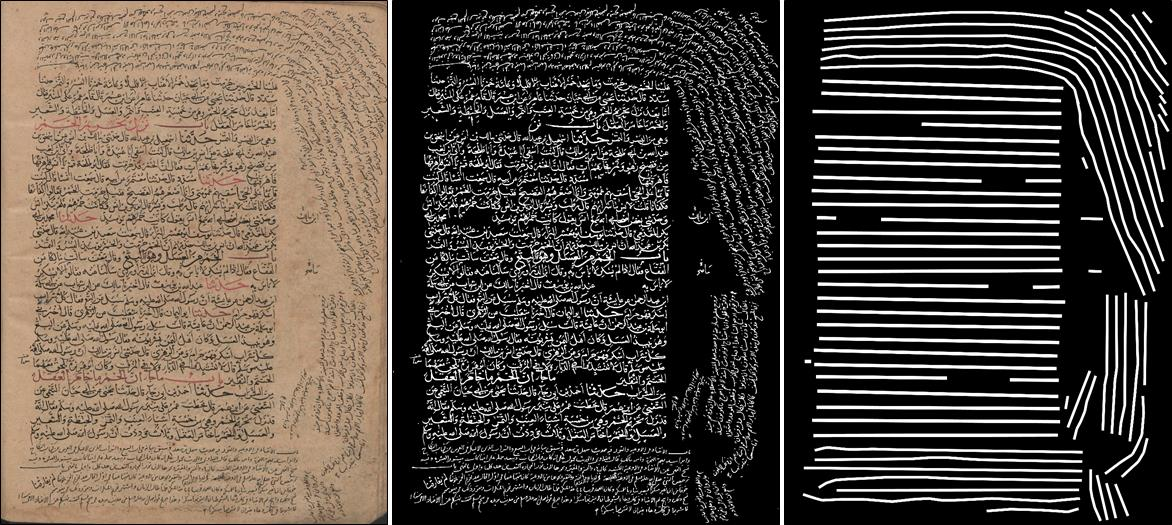
\includegraphics[width=12cm]{images/fcn_image.jpg}
    \caption{A sequence of original, binarized, and labeled document images}
    \label{fig:fcn_image}
\end{figure}
\begin{figure}[!htb]
    \centering
    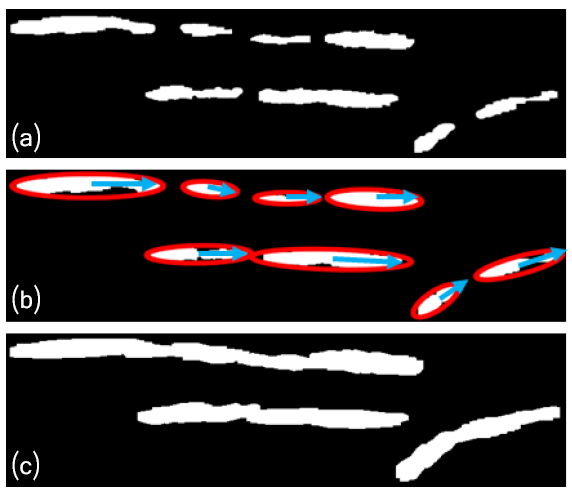
\includegraphics[width=7cm]{images/FCN_post.png}
    \caption{Post processing phases: (a) Predicted line mask may have disconnected components. (b) For each component, an ellipse (red) is fitted and its orientation vector $\theta$ (c) (blue) is computed. (c) Morphological dilation is applied to each component with a narrow kernel in the direction of its fitted ellipse.}
    \label{fig:fcn_post}
\end{figure}

\noindent
This paper \cite{PP} presented an approach for line and character segmentation based on the \acrshort{pp} method. This method was applied to a historical Arabic manuscript collected from the manuscripts department at Umm Al-Qura University’s Library.
 \begin{figure}[!htb]
    \centering
    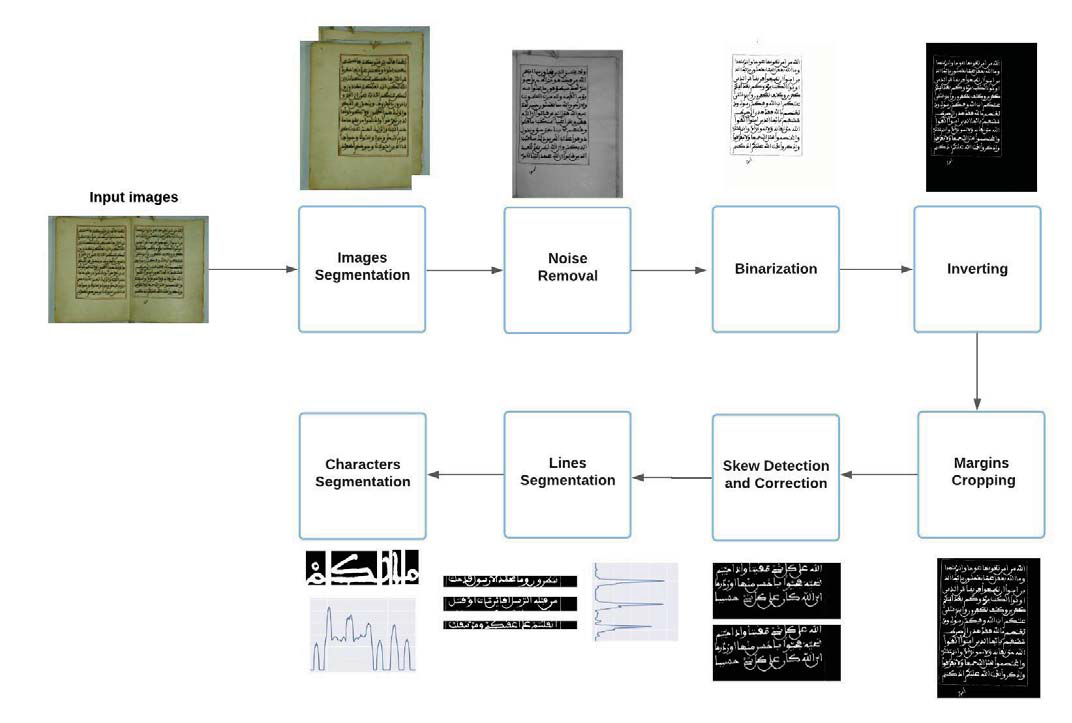
\includegraphics[width=11cm]{images/pp_seg.png}
    \caption{Process of proposed method for line and word segmentation.}
    \label{fig:pp_seg}
\end{figure}
\newline\\
In order to reach excellent segmentation results, it is needed to apply some preprocessing steps to the manuscript such as images Extraction, noise Removal, binarization and inverting, margins cropping, skew detection, and correction then segmentation. The segmentation step is dividing text images into base components such as lines, words, and characters.
\begin{itemize}[labelindent=1em,labelsep=0.25cm,leftmargin=*]

        \item[\char `A)] \textbf{Lines Segmentation:-}\\
         After the images’ margins have been cropped, images are segmented line by line using the Horizontal \acrshort{pp} method, which converts 2D into 1D images by calculating the densities of each row. Then, each line is cropped separately at the lowest density point. Since the manuscript is written in a complex way, the spaces between lines is not totally empty. Therefore, its density from Horizontal \acrshort{pp} is not equal to 0. In order to overcome this problem, an opening operation is performed on each image before segmentation. Opening is considered a morphology operation.
        
        \item[\char `B)] \textbf{Characters Segmentation:-}\\
        Another type of segmentation that was performed is character segmentation. In this step, the lines that are obtained from the previous step are divided into separated characters.
        
        This step was applied by using the Vertical \acrshort{pp} method. This method works the same way as Horizontal \acrshort{pp} in the previous step, except that the direction of calculating the density. In Vertical \acrshort{pp} it is calculated on columns instead of rows. The opening operation was also performed on each line before segmentation.
    \end{itemize}

\noindent
The total number of lines segmented during lines segmentation is 635. The original manuscript contains 657 lines. There were 10 empty segmented lines out of 635. since they contain
parts of the characters from the line above and below them.
Figure \ref{fig:pp_empty} shows an example of this case. In addition, 15 lines
were overlapped with other lines. Table \ref{table:1} shows the results
summary of lines segmentation.

\begin{figure}[!htb]
    \centering
    
\includegraphics[width=11cm]{images/pp_empty.png}
    \caption{Empty line.}
    \label{fig:pp_empty}
\end{figure}

\begin{table}[!htb]
\centering
\begin{tabular}{|l|l|}
\hline
\textbf{Case}                   & \textbf{Number of Lines} \\ \hline
Total number of segmented lines & 635                      \\ \hline
Correctly segmented             & 610                      \\ \hline
Empty                           & 10                       \\ \hline
Two overlapped                  & 11                       \\ \hline
Three overlapped lines          & 4                        \\ \hline
\end{tabular}
\caption{Lines segmentation results summary.}
\label{table:1}
\end{table}


\section{Word Segmentation}
Word/subword segmentation is an important step in the segmentation phase for segmentation-based Arabic \acrshort{ocr}(\acrshort{aocr}) systems since it facilitates working on the character segmentation stage. In addition, it can be employed as a post processing stage after character recognition to increase the recognition rate.\\

In paper \cite{article} 
introduced a segmentation algorithm that uses a technique in which the overlapping Arabic words/sub-words are horizontally separated; they also used a feedback loop between the character segmentation stage and final recognition stage. 

In paper \cite{jawad_h_alkhateeb}
proposed a method for baseline detection and employed it to extract the connected components of each sub-word. After detection of the baseline, an iterative process was used to detect the connected components based on the connected black pixels in the sub-word. \\

\noindent
Arabic writing is cursive; therefore, words and subwords are separated by spaces, so word boundaries are always represented by a space. According  to  this, distances between each pair of consecutive sub-words are obtained. Normally the distances between words are larger than the distances between subwords, thus words can be segmented by comparing this distance against a suitable threshold. This paper is concerned with word segmentation using vertical histogram and connected component analysis. Also, distance  information is very essential in segmenting words. Here, the distances between subwords were measured and compared to an optimal threshold to determine if the distance corresponds to the separation of two words or not. 

\begin{itemize}[labelindent=1em,labelsep=0.25cm,leftmargin=*]
        \item[\char `A)] \textbf{Baseline Detection:-}
        Before  segmenting  the  Arabic  words,  we  need  to detect  the  baseline  as  it  is  believed  that  this  baseline  is  very  essential  in  analyzing  Arabic  text.  Since  the  Arabic  letters  are  usually written along the baseline, hopefully, there should be a peak in the baseline position when we project the written line along the vertical axis of the image.
        The  improved result is shown in figure \ref{fig:basline}
 
         \begin{figure}[!htb]
            \centering
            
\includegraphics[width=6cm]{images/basline.png}
            \caption{Baseline detection: original result using only vertical projection using both vertical projection and knowledge-support}
            \label{fig:basline}
        \end{figure}
        
        \item[\char `B)] \textbf{Extracting Connected Components and Sub-Words:-}
        
        Segmentation is an essential step that separates the text image objects for the recognition phase. The typical segmentation for the printed binary document is based on the histogram projection analysis and regrouping of the connected components. Arabic writing is cursive  and is such that words are separated by spaces. However,  a  word may contain several sub-words which are a portion  of  the  word including one or more connected letters.
Figure \ref{fig:subword} shows three Arabic words consisting of one, two, and three sub-words respectively. 

 \begin{figure}[!htb]
    \centering
    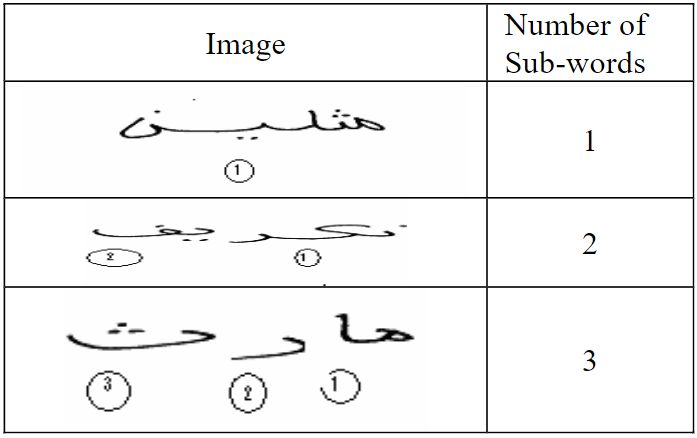
\includegraphics[width=5cm]{images/subword.png}
    \caption{Arabic words with sub-words}
    \label{fig:subword}
\end{figure}

The connected components (\acrshort{cc}s) for the line image must be determined.  The  \acrshort{cc}s  are  rectangular  boxes  bounding  together  regions of connected objects. The objective of the \acrshort{cc}s phase is to  form  rectangles  around  the  connected object on the image. The algorithm used to obtain the \acrshort{cc}s  are  the  iterative procedure that compares any black pixels in any pair of the line are connected together. Bounding rectangles are  extended to enclose any grouping  of connected black pixels. Figure \ref{fig:ccs}(a) shows the output of the \acrshort{cc}s. With extracted connect components,sub-words are segmented as follows. Firstly, small parts like dots in the image  are  temporally  ignored. Secondly, components whose coordinates are overlapped on the x-axis are merged to obtain a combined large  component, namely a sub-word. Thirdly, the distance of each pair of consecutive sub-words is obtained, which will be used to segment words in the next section.
\begin{figure}[!htb]
    \centering
    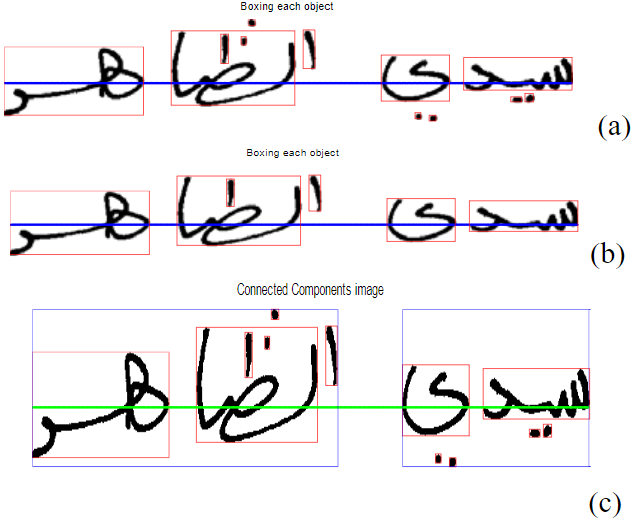
\includegraphics[width=6cm]{images/ccs.png}
    \caption{Examples of extracted connected components (a), sub-words of combined components (b), and detected words (c)}
    \label{fig:ccs}
\end{figure}




\end{itemize}

\noindent
The table \ref{tb:vpp-accuracy-table}shows the testing results of this technique which is tested on 200 images in the test set and the segmentation accuracy is  85\%.
    

\begin{table}[!htb]
\centering
\begin{tabular}{|l|l|l|l|l|}
\hline
 NO .of Images & Correct Seg. & Under Seg. & Over seg. & Misplaced Seg. \\ \hline
 200  & 85\%  & 90\% & 4\% & 2\% \\ \hline
\end{tabular}
\caption{Results of the accuracy of segmentation}
\label{tb:vpp-accuracy-table}
\end{table}

\section{Word Spotting}
Since, \acrshort{ocr} for manuscript images is impossible, this is due to the semi-cursive nature of Arabic script which is very difficult to explore by algorithms and image processing methods.

\noindent
Word spotting techniques are used to explore and research in the content of Arabic manuscript images. It’s about characterizing segmented handwritten words with a set of points of interest by providing a means of identification and research in these manuscripts. Each word segmented and described by key features will be compared to query words. \\

In \cite{Noureddine} presents a method that facilitates access to the content of images. This method is based on the invariant local detectors and descriptors (scale, rotation, brightness variations) for the detection of this information in the Arabic manuscripts. Word spotting technique allows the matching process between the handwritten words of the query images with the target images. 

The proposed method for the characterization of images of Arabic manuscripts. In the same way, as in the field of the recognition of Latin texts shown in the figure \ref{fig:noureddine-word-spotting-results}.
\begin{figure}[!htb]
    \centering
    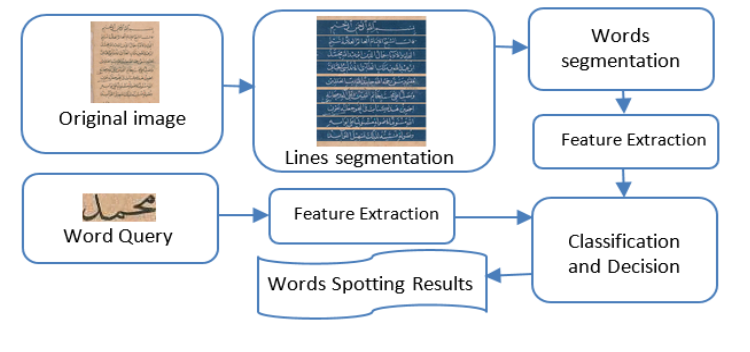
\includegraphics[width=13cm]{images/noureddine-word-spotting.png}
    \caption{Process of the proposed method for word spotting}
    \label{fig:noureddine-word-spotting}
\end{figure}

\begin{itemize}[labelindent=1em,labelsep=0.25cm,leftmargin=*]
        \item[\char `A)] \textbf{Acquisition and Pre-processing:-} \\
        They collect manually huge scanned manuscripts, then a  series of pre-processing can be applied to images such as Contrast Enhancement, straightening, curvature correction, detail emphasis, and spreading of levels. This processing can improve the quality of the images and also their segmentation. An example of the collected data after preprocessing shown in the figure \ref{fig:noureddine-data}
        \begin{figure}[!htb]
            \centering
            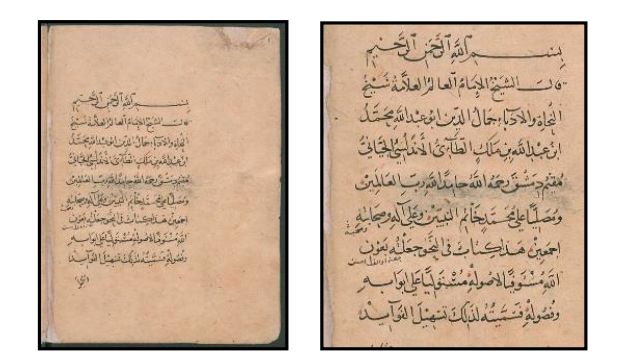
\includegraphics[width=10cm]{images/noureddine-data.png}
            \caption{Example of the scanned image left and right after pre-processing}
            \label{fig:noureddine-data}
        \end{figure}
        
        \item[\char `B)] \textbf{Lines Segmentation:-} \\
        Line segmentation is necessary to locate the position of words for the word spotting method. The line was extracted using grayscale images to facilitate line detection despite some overlaps. They used the projection algorithm in \cite{ManmathaProjectionAlgorithm}. The projection function $f(y)$ that has applied for a gray level image of intensity $I(x, y)$ is as follows:
        \begin{equation}
            f(y) = \sum_{x=0}^w I(x, y)
        \end{equation}
        
        The project profile $f(y)$ of the image $I$ for the line x is illustrated in the figure \ref{fig:noureddine-word-line}. Additional high-frequency noise may affect this function. In this case, it is necessary to smooth this signal with the aid of a filter, we can perform a convolution with a Gaussian filter in the equation \ref{equ:gaussian-filter} in order to eliminate the high-frequency noise in the signal of the function in the equation \ref{equ:signal-function}
        
        \begin{equation}
            p(y) = f(y)*g(y,\sigma) 
        \label{equ:gaussian-filter}
        \end{equation}
        
        \begin{equation}
            g(y, \sigma) = \frac{1}{\sigma \sqrt{2 \pi}} e^{-\frac{y^2}{2\sigma^2}}
        \label{equ:signal-function}
        \end{equation}
        
        \item[\char `C)] \textbf{Word Segmentation:-} \\
        In order to extract all the information in each word to facilitate the task to the processing algorithms. Some image preprocessing techniques like applying binary images for the extraction of the related components, then morphological dilation of the binary images allows the fusion of the isolated characters and the pseudo-words. The projection at each line provides the words. The main problem with this technique is its sensitivity to overlapping words. Detection of the related components at the level of each line in the binary images to also locate the words.
        The following figure \ref{fig:noureddine-word-line} shows an example of segmentation of elements (isolated characters, pseudo words, and words).
        
        \begin{figure}[!htb]
            \centering
            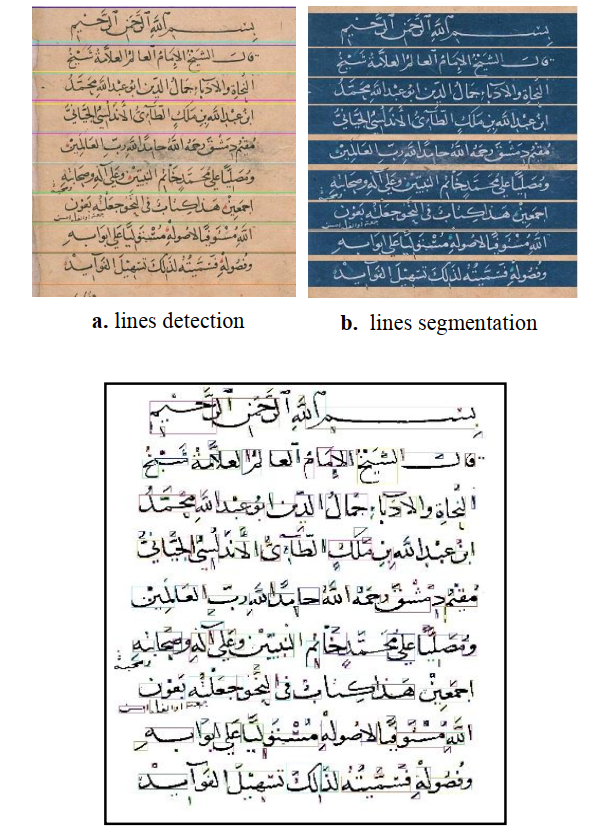
\includegraphics[width=8cm]{images/noureddine-line-word-segmentation.png}
            \caption{Segmentation results}
            \label{fig:noureddine-word-line}
        \end{figure}
        
        \item[\char `D)] \textbf{Feature Extraction:-} \\
        As part of the Word Spotting method of detecting words at the level of Arabic handwriting, all types of manuscripts must be considered. However, some documents, such as manuscripts with different colors but with identical intensities, require the use of color to ensure correct key points extraction. The second possible variation concerns the relationship between the reliability and the algorithmic cost of the detector. Indeed, the SIFT detector extracts robust and fewer points but at the cost of additional calculations. In this case, the use of SURF detectors to extract feature elements (isolated characters, pseudo words, or words) can be effective and is faster compared to other detectors
        
        \item[\char `E)] \textbf{Classification, Matching and Decision:-} \\
        By using SURF interest points. The comparison between two interest points can be done with several methods. Choice of such a method can be made per processing costs. Interest points are characterized by their properties. The comparison can therefore be carried out in two stages: The first step of comparison between two points is carried out by examining the signs of traces of the Hessian matrix. The sign of the trace of the Hessian matrix thus represents the sign of the Laplacian and the meaning of blobs. The second step of the comparison consists in calculating the distance between the descriptor vectors of the two interest points. The most commonly used comparison methods are based on correlation and on the calculation of vector distances. The distance between two vectors v and u of the two descriptors of interest points can be calculated with the Euclidean distance or with the Mahalanobis distance.
        \item[\char `F)] \textbf{Results and application GUI:-} \\
        The results of matching with the Word Spotting method give many occurrences of the name "Mohamed \<محمد>" equal to twice shown in figure \ref{fig:noureddine-word-spotting-results}. We used three types of query images (color, grayscale and binary) and we got the same result. Therefore, this method can be applied to a set of images of the same manuscript, which makes it possible to search all the occurrences of the query word

        \begin{figure}[!htb]
            \centering
            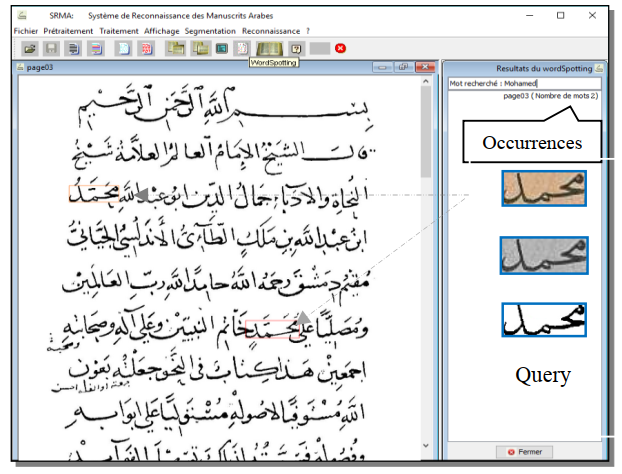
\includegraphics[width=12cm]{images/noureddine-word-spotting-application.png}
            \caption{Word spotting results}
            \label{fig:noureddine-word-spotting-results}
        \end{figure}

\end{itemize}

\clearpage

\section{Implementation Approach}
After reviewing different papers addressing the problem of digitizing historical Arabic manuscripts documents, as previously mentioned, that \acrshort{htr} systems are inefficient for recognizing the historical handwritten documents, so we decided to follow the approach of the pattern recognition technique to build an intelligent system able to understand handwritten manuscript documents by matching the pattern with manually collected huge labeled data of segmented words. 
Since the goal of this system is to digitize the image manuscripts, then word spotting will not be enough for that purpose as the aim of word spotting is to final all the instances of a query word in a dataset of images. We need also a word recognition technique to recognize the content of the word image. So we will use a special text-embedded technique to extract textual features to produce a common representation that enables the machine to recognize and extract it when having a particular image feature. \acrfull{phoc} is a new method to achieve this scenario which encodes if a particular character appears in a particular spatial region of the string \cite{WORDSPOTTING}. We will use this method with a modified version. \\


We have decided to go through VML-HD dataset \cite{VMLHD}, as it has a lot of images for different Arabic manuscripts and different fonts with different styling word shapes, we will do data cleaning to remove mislabeled data and to prepare it for word spotting techniques. In addition, we will augment the data using morphology techniques for image preprocessing that's because it's unbalanced and has low correlations with the number of collected words. \\

In word and line segmentation, we want to segment the line first, so we will use morphology operations after doing some preprocessing like normalization, binarization, median filtering logic,  dilation, and erosion for edge detection improvement, then we finally extract the contours from dilation operation as segmented lines. In word segmentation, we will use morphological operation techniques to extract each word of the line as cropped image \cite{PP}.
\chapter{System Design and Architecture}
\label{ch:system-design}
\quad In this chapter, there is a full description of each module design and architecture in our project. First, an overview and any needed assumptions we used will be explained. Then the overall system architecture and block diagram. Then for each module, there is a functional description, modular decomposition, design constraints, and any other needed descriptions. In addition to the decisions, we took about the modules' functionalities. \\

During the development and implementation of our project, we made sure the project code is modular and clear enough to be understood, in case of any future need for the code itself.

\bigskip
\noindent 
The overall system could be broken down to mainly 4 components:
\begin{itemize}[itemsep=1pt, topsep=5pt]
    \item \textbf{Page segmentation}: Computer vision techniques to prepare unseen handwritten image pages to be extracted into lines and words.
    \item \textbf{Model development}: End-to-end deep learning network used to predict and recognize unseen segmented manuscript images.
    \item \textbf{Applications development}: Web and mobile applications developed and integrated with deep learning networks as user-friendly services. 
    \item \textbf{Testing}: Set of scripts, programs, and \acrfull{gui} for system testing and development. 
\end{itemize}

This chapter discusses the first 2 modules, while the applications development and testing are discussed in chapters \ref{ch:system-development} and \ref{ch:system-testing}, because it's not part of the final deployed system, but rather built for testing and development purposes.

\section{Overview and Assumptions}
\acrshort{asar} project consists of 3 main modules that need to be completely understood before starting implementing such a thing. These three are line segmentation, word segmentation, and pattern recognition. Apart from that, there is the connection between each module and the other, the research and modularity that needs to be considered. Each of these modules is described in detail in the following section, and how they all connect to each other, and how they represent the system architecture. \\

\noindent
Some assumptions are also considered in delivering this project are: 
\subsection{Accuracy}
Since the Arabic language has difficult problems to deal with such as styling format that is different from writer to writer, and from age to age.
We will use the hybrid technology to introduce a good accuracy in recognizing Arabic words or characters in whatever style are writing.

\subsection{Speed}
The system will try to recognize the manuscript documents have a lot of lines and words in a reasonable time. 

\subsection{Friendly Interface}
The system is developed into two (web and mobile) applications with a friendly interface that gives the user the accessibility to have an account, upload, crop, and download the document results.

\section{System Architecture}
% The aronal fieldchitecture of your system should be given in this section. This architecture should be first represented as a block diagram (subsection 5.2.1), which clarifies different project modules and the connections between them. You may add more subsections to properly explain your design. If possible, flowcharts are better included to ensure that the big picture and the interaction between different modules are very clear to the reader. Thereafter, each module should have a separate subsequent section to clearly describe and discuss it.

The system's main modules can be explained in this flow:
\begin{itemize}[itemsep=1pt, topsep=5pt]
    \item Image Preprocessing
    \item Page Segmentation
    \begin{itemize} 
        \item Line Segmentation
        \item Word Segmentation
    \end{itemize}
    \item Word Spotting
    \item Model Development
\end{itemize}

\noindent
In image preprocessing, we will prepare the manuscript image to be passed into the next module by applying some morphological operations such as normalization, adaptive thresholding, and median subtraction. After the image is preprocessed, we will extract each line segment by using the contours of the image, then we will take the largest contours area as segmented lines. The output of these lines will go into a vertical projection algorithm to extract each word in this which has the lowest histogram to separate between words. \\

\noindent
After each word is extracted from the manuscript image, it will be embedded into the trained model to analyze and predict the corresponding transcript. Model development, image preprocessing, line, and word segmentation are explained in detail in the following subsections.

\newpage
\section{Block Diagram}

\begin{figure}[!htb]
    \centering
    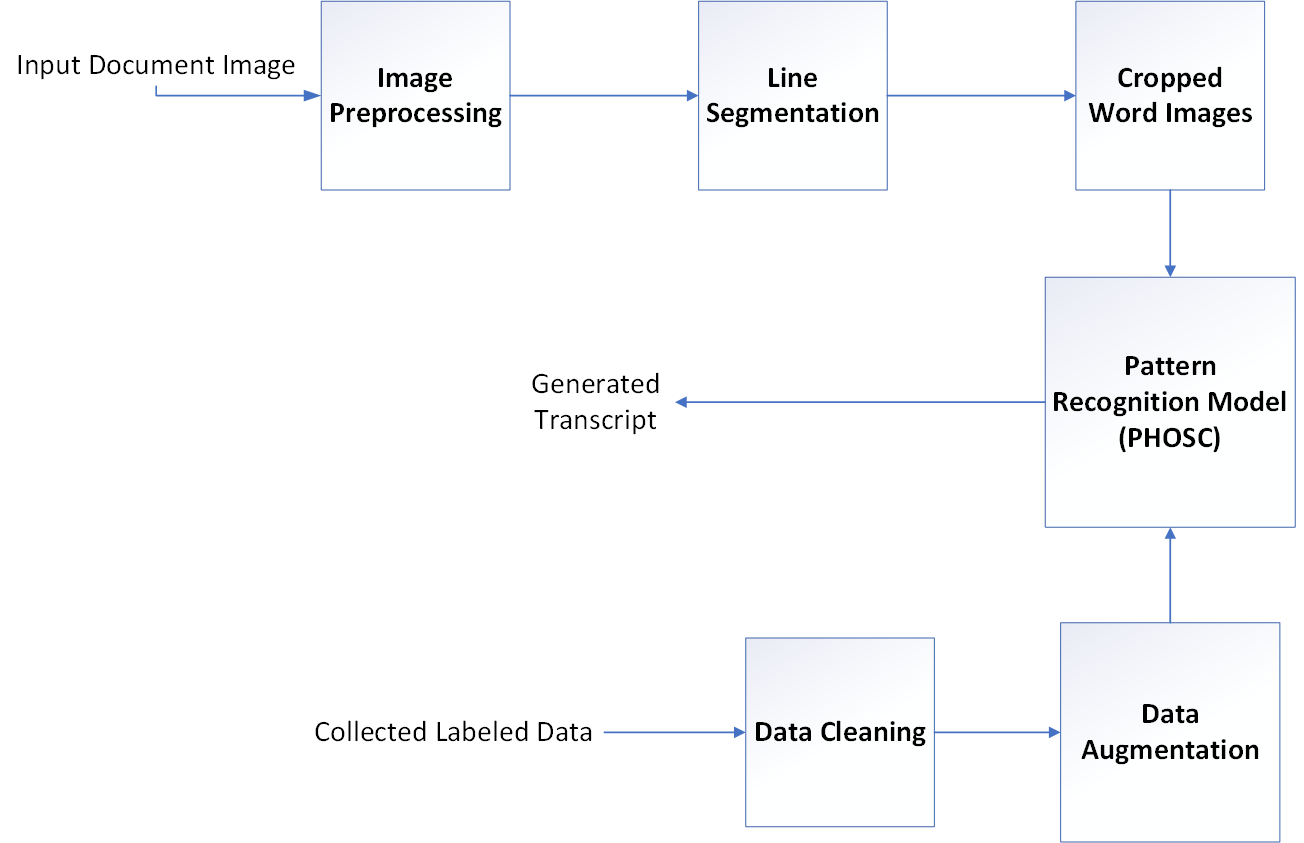
\includegraphics[width=14cm]{images/block diagram.png}
    \caption{ASAR Architecture Block Diagram}
    \label{fig:block-digram}
\end{figure}

\section{Image Preprocessing}
This module is responsible for preprocessing techniques that are used in document images as an initial step in the segmentation system. Most of preprocessing techniques are application-specific and not all preprocessing techniques have to be applied to all applications. Each application may require different preprocessing techniques depending on the different factors that may affect the quality of its images, such as those we applied to images for segmentation.

\subsection{Functional Description}
Preprocessing is the preliminary step that transforms the data into a format that will be more easily and effectively processed. Therefore, the main task in preprocessing the captured data is to decrease the variation that causes a reduction in the efficiency  rate and increases the complexities, for example, preprocessing of the input raw stroke of characters is crucial for the success of efficient character recognition systems. Thus, preprocessing is an essential stage prior to controlling the suitability of the results for the successive stages. 


\subsection{Modular Decomposition}
Image enhancement improves the quality of images for human perception by removing noise, reducing blurring, increasing contrast, and providing more detail. This section will provide some of the techniques used in image enhancement In \cite{inbook}. 

\begin{itemize}[labelindent=1em,labelsep=0.25cm,leftmargin=*]
        \item[\char `A)] \textit{\textbf{Resize Image}}\\
        Images are normalized into a specific size, decided empirically or experimentally depending on the application and the feature extraction or classification techniques used, then features are extracted from all images  with the same size in order to provide data uniformity. 
        \item[\char `B)] \textit{\textbf{Normalization}}\\  
        The Histogram Equalization \cite{equalization} evenly distributes the occurrence of pixel intensities so that the entire range of intensities is considered. This method usually increases the global contrast of images, especially when the usable data of the image is represented by close contrast values. Through this adjustment, the intensities can be better distributed on the histogram. This allows for areas of lower local contrast to gain a higher contrast. Histogram equalization accomplishes this by effectively spreading out the most frequent intensity values. Then probability density function (pdf) is calculated for the histogram shown Fig.\ref{fig:equalize}.
        \begin{figure}[!htb]
            \centering
            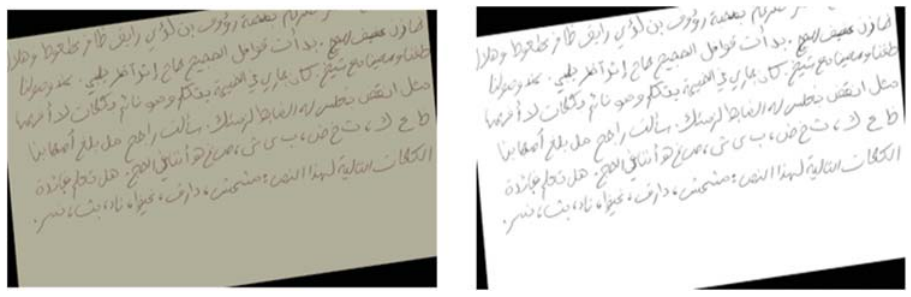
\includegraphics[width=11cm]{images/equalize.png}
            \caption{Affective result of proposed adaptive histogram equalization}
            \label{fig:equalize}
        \end{figure}
        \item[\char `C)] \textit{\textbf{Gaussian Blur}}\\ 
        applying a Gaussian filter of a standard deviation   $\sigma$ for noise
        reduction purposes, the gradient magnitude is then computed using the
        simple energy function:
        
        \begin{equation}
            e(I) = [\frac{\partial}{\partial x} I] + [\frac{\partial}{\partial y} I]
            \label{equ:blur}
        \end{equation}
        \item[\char `D)] \textit{\textbf{Gray Scaling}}\\
        A grayscale (or graylevel) image is simply one in which the only colors are shades of gray. The reason for differentiating such images from any other sort of color image is that less information needs to be provided for each pixel.so, it is only necessary to specify a single intensity value for each pixel, as opposed to the three intensities needed to specify each pixel in a full-color image.
        grayscale images are entirely sufficient for an easy process and so there is no need to use more complicated and harder-to-process color images.
        
        the input RGB fundus image $(I)$ is converted to a grayscale image ($Ig$) using Eq.\ref{equ:gray}.
        
        \begin{equation}
            Ig = 0.2989 * IR + 0.5870 * IG + 0.1140 * IB
            \label{equ:gray}
        \end{equation}
        \item[\char `E)] \textit{\textbf{Gaussian Thresholding (OTSU)}}\\
        The goal of thresholding \cite{thresholding} an image is to classify pixels as either “dark” or “light”.\\
        There are numerous methods for image thresholding which already been used by some researchers. The most common thresholding method has been proposed by Otsu . Otsu’s method works better where the clear separation between foreground and background exists or where image illumination is not variable shown in Fig \ref{fig:otsu}. However, real-life images possess especially in handwriting images various kinds of degradations (e.g. illumination contrast, skewed, stains, and noise) that weaken the thresholding proposed by Otsu’s. Gaussian thresholding (OTSU) with binary inverse shown in Fig.\ref{fig:otsubnv}.
        \begin{figure}[!htb]
            \centering
            \includegraphics[width=11cm]{images/otsu.png}
            \caption{Images results of various thresholding methods}
            \label{fig:otsu}
        \end{figure}
        
        \begin{figure}[H]
            \centering
            \includegraphics[width=7cm]{images/otsu-binv.png}
            \caption{Gaussian thresholding (OTSU) with binary inverse}
            \label{fig:otsubnv}
        \end{figure}
         \item[\char `F)] \textit{\textbf{Median Subtraction}}\\
         Removing noise is to remove information coming from the
        background such as show-through effects, interfering strokes
        due to the seeping of ink during a long period of storage, spots of
        humidity and curvature effect. Example for the image before
        using the filter method shown in Fig.\ref{fig:bfmed} 
        
        \begin{figure}[!htb]
            \centering
            \includegraphics[width=9cm]{images/bmedian.png}
            \caption{Before using filter}
            \label{fig:bfmed}
        \end{figure}
        
        In median filtering \cite{median}, the neighboring pixels are ranked
        according to brightness (intensity) and the median value
        becomes the new value for the central pixel, shown in Fig.\ref{fig:afmed}.
        the value of an output pixel is determined by the median of the
        neighborhood pixels.
        
        \begin{figure}[!htb]
            \centering
            \includegraphics[width=9cm]{images/afmedian.png}
            \caption{Using median filter}
            \label{fig:afmed}
        \end{figure}
    \end{itemize}

\section{Line Segmentation}
This module is responsible for applying the text-line segmentation technique. Text-line segmentation is recognized as being an important step for handwritten text recognition because inaccurate segmentation will cause errors in the recognition step. %..

\subsection{Functional Description}
In this module, we will apply our method for text-line segmentation. Fig \ref{fig:flow_line} shows the flowchart of the proposed system. The proposed method consists of two stages. In the first stage, the mathematical morphology technique is used for constructing bridges between the components. In the next stage, find contours technique is proposed for the segmentation of the text into lines.
        \begin{figure}[!htb]
            \centering
            \includegraphics[width=14cm]{images/flowchart_line_segmentation.png}
            \caption{Flowchart of the proposed line segmentation method. }
            \label{fig:flow_line}
        \end{figure}
\subsection{Modular Decomposition}
This module could be separated into two distinct sub-modules depending on each other, and we will discuss them in detail. %..

\subsubsection{Morphology}
Mathematical morphology is a tool for extracting image components that are useful in the representation and description of region shapes, such as boundaries, skeletons, and the convex hull. Dilation is a primitive morphological operation that grows or thickens objects in a binary image. The specific manner and extent of this thickening is controlled by a shape referred to as a structuring element. Structuring elements are small sets or sub-images used to probe an image under study for properties of interest.

There are two basic morphological operators: erosion and dilation. These operators are usually applied in tandem. Opening and closing are two derived operations defined in terms of erosion and dilation.

\begin{itemize}
        \item {\textbf{Erosion:}}
            The erosion operation uses a structuring
            element for reducing or shrinking the shapes contained in the input image:
        
            \begin{equation}
                 A \ominus B = \left\{Z |  B_{z} \subset A \right\}
                \label{equ:Erosion-function}
                \end{equation}
            where A is the image, B is the structure element, and z is the points in B.
                
    \item {\textbf{Dilation:}}
            The dilation operation uses a structuring element characteristics for expanding the image:
        
            \begin{equation}
                A \oplus  B = \left\{Z |  B_{z} \bigcap  A \neq \phi  \right\}
                \label{equ:Dilation-function}
            \end{equation}
            where A is the image, B is the structure element, and z is the points in B.
            \item {\textbf{Opening:}}
            The opening is defined as an erosion followed by a dilation using the same structuring element. Opening of a grey-level image A and structuring element B, denoted \textbf{A $\circ $ B} , is defined as follows:
        \begin{equation}
            A \circ  B = \left ( A \ominus B \right ) \oplus B
            \label{equ:Opening-function}
        \end{equation}
            
            \item {\textbf{Closing:}}
            Closing is defined as a dilation followed by an erosion using the same structuring element for both operations. Closing of a grey-level image A and structuring element B, denoted \textbf{A $\bullet$ B} , is defined as follows:
        \begin{equation}
            A \bullet B = \left ( A \oplus   B \right ) \ominus B
            \label{equ:Clocing-function}
        \end{equation}
            
    \end{itemize}
\noindent
As it can be seen above and in general in any morphological operation the structuring element used to probe the input image, is the most important part.

\noindent
A structuring element is a matrix consisting of only 0's and 1's that can have any arbitrary shape and size. Typically are much smaller than the image being processed, while the pixels with values of 1 define the neighborhood. The center pixel of the structuring element, called the origin, identifies the pixel of interest – the pixel being processed.
\noindent
For example, Fig.\ref{fig:structuring-element} illustrates a diamond-shaped structuring element of 7x7 size.
\begin{figure}[!htb]
    \centering
    \includegraphics[width=5cm]{images/SE.png}
    \caption{A Diamond-Shaped Structuring Element and its Origin}
    \label{fig:structuring-element}
\end{figure} \\


To begin with, a set of sequential morphological operators is applied to the binary image Fig \ref{fig:input_binary_img} to extract points that have high gradients to their background as the contrast feature and to obtain a processed image version, with the intention that every connected pixel component represents a text line.Fig \ref{fig:Flowchart_MO} shows the whole procedure of our novel morphology-based technique to extract the feature. The series of morphological operations will be discussed in the following:%Done
\begin{figure}[H]
    \centering
    \includegraphics[width=6cm, height=9cm]{images/input.png}
    \caption{Binary Images that are the input to morphological operations}
    \label{fig:input_binary_img}
\end{figure}

\begin{itemize}
        \item[\char `a)] \textit{\textbf{Closing}}
         
         A closing is used to close holes inside of objects or for connecting components together.Fig \ref{fig:closing} shows the result after applying the closing on the binary input  image.
         
         The closing operation has filled in gaps that are smaller than or the same size as the structuring element. Hence, the closing could be useful for connecting objects that are near each other, while not affecting objects that are too far apart.

        \begin{figure}[!htb]
             \centering
             \begin{subfigure}[b]{0.4\textwidth}
                 \centering
                 \includegraphics[width=6cm, height=9cm]{images/clos1.png}
                 \caption{closing: [20,5]}
                 \label{fig:close1}
             \end{subfigure}
             \hfill
             \begin{subfigure}[b]{0.4\textwidth}
                 \centering
                 \includegraphics[width=6cm, height=9cm]{images/clos2.png}
                 \caption{closing: [35,1]}
                 \label{fig:close2}
             \end{subfigure}
            \caption{Applying a morphological closing operation to our input image.}
            \label{fig:closing}
        \end{figure}

        \item[\char `b)] \textit{\textbf{Erosion}}
        
        We have used morphological operations, mainly, erosion to extract the useful foreground and background information. Erosion is one of two fundamental operations in morphological image processing from which all other morphological operations are based. For details about this see \cite{esosion}. After Closing, we will have a smoothed image, where the foreground part belongs to black text regions and the background part consists of white regions. By erosion, we determine some important information from the foreground and background portions which are very helpful in our line segmentation purpose.
        
        Fig \ref{fig:erosio_img} shows the result after applying the erosion to our image after the closing step.

        \item[\char `c)] \textit{\textbf{Blurring}}
        When we blur an image, we make the color transition from one side of an edge in the image to another smooth rather than sudden. So, we’ll do is apply an average blur on the image after erosion  using a 99 x 1 kernel. This will help smooth out high-frequency noise in our image. A blur is a very common operation we need to perform before other tasks such as thresholding.
        
        This Fig \ref{fig:Blurring} shows this operation.
        
         \begin{figure}[!htb]
             \centering
             \begin{subfigure}[b]{0.4\textwidth}
                \centering
                \includegraphics[width=6cm, height=9cm]{images/erosion.png}
                \caption{Applying erosion to our image}
                \label{fig:erosio_img}
             \end{subfigure}
             \hfill
             \begin{subfigure}[b]{0.4\textwidth}
                \centering
                \includegraphics[width=6cm, height=9cm]{images/blureImg.png}
                \caption{Blurring to our image}
                \label{fig:Blurring}
             \end{subfigure}
            \caption{The sample after applying erosion and blurring}
            \label{fig:erosion-blurring}
        \end{figure}
        
        
        \item[\char `d)] \textit{\textbf{Thresholding}}
        The thresholding is a key step in our segmentation method, its aim is to threshold the resulting smoothed image in order to isolate the blobs corresponding to line components.
        
        Now, we can apply Simple Thresholding to Blurred images as shown in Figure \ref{fig:treshold_img}.
        
        \begin{figure}[H]
            \centering
            \includegraphics[width=6cm, height=9cm]{images/threthold.png}
            \caption{Applying simple thresholding.}
            \label{fig:treshold_img}
        \end{figure}
        
        \item[\char `e)] \textit{\textbf{Dilation}}
        Finally, We applied the dilation operation on the Thresholding image to make objects more visible and fill in small holes in objects. Lines appear thicker, and filled shapes appear larger. Dilation makes the groups of text to be detected more accurately as shown in the Fig \ref{fig:Dilation_img}.%Done
        
        \item[\char `f)] \textit{\textbf{Labeling}}
        This step aims to show all connected regions in the dilated image by applying connected-component labeling as shown in the Fig \ref{fig:Labeling_img}.
        \\
        Connected Component Labeling solves the problem of finding out parts of the image that are connected physically, irrespective of color.
        
        \begin{figure}[!htb]
             \centering
             \begin{subfigure}[b]{0.4\textwidth}
                \centering
                \includegraphics[width=6cm, height=9cm]{images/dilation.png}
                \caption{Applying dilation. }
                \label{fig:Dilation_img}
             \end{subfigure}
             \hfill
             \begin{subfigure}[b]{0.4\textwidth}
                \centering
                \includegraphics[width=6cm, height=9cm]{images/21_labels2.png}
                \caption{Connected component labeling.}
                \label{fig:Labeling_img}
             \end{subfigure}
            \caption{The sample after applying dilation and connected component labeling}
            \label{fig:dialation-and-ccl}
        \end{figure}
        

\end{itemize}

\begin{figure}[!htb]
    \centering
    \includegraphics[width=11cm]{images/Flowchart_MO.png}
    \caption{Flowchart of the proposed method to extract contrast features for text line detection}
    \label{fig:Flowchart_MO}
\end{figure} 


\subsubsection{Finding Contours}

After the completion of the first stage, the next stage is to extract individual text lines present in the image. In order to extract individual text lines, a technique based on finding contours is used.\\

Contours are typically used to find a white object from a black background. All the above morphological operations are applied so that the Contours can detect the boundary edges of the blocks of text of the image.\\

Now, we can find all contours in the dilated image, check all the areas of each of the contours to identify which contours represent the text line and draw these contours to show all text lines in the image as shown in this Fig \ref{fig:drawing}.

We can crop all these contours to extract individual text lines from an image as shown in this Fig \ref{fig:crop}.

\begin{figure}[!htb]
     \centering
     \begin{subfigure}[b]{0.4\textwidth}
        \centering
        \includegraphics[width=6cm, height=9cm]{images/22_imgContoure1.png}
        \caption{After drawing contours.} 
        \label{fig:drawing}
     \end{subfigure}
     \hfill
     \begin{subfigure}[b]{0.4\textwidth}
        \centering
        \includegraphics[width=6cm, height=9cm]{images/lines_text.drawio.png}
        \caption{After cropping.} 
        \label{fig:crop}
     \end{subfigure}
    \caption{The sample after drawing contours and cropping}
    \label{fig:drawing-contours-cropping}
\end{figure}


\section{Word Segmentation}
the process of dividing the written text into meaningful units, such as words, and determining the word boundaries in a sentence or a document by computer algorithms.

\subsection{Functional Description}
 The cursive nature of the Arabic script such as the existence of different shapes for each character according to its location in the world besides the existence of diacritics makes Arabic character segmentation a very challenging task. A robust character segmentation algorithm for printed Arabic text with diacritics is developed based on the contour extraction technique. The algorithm works by extracting the up-contour part of a word and then identifies the splitting areas of the word characters. 

\subsection{Modular Decomposition}

\begin{itemize}[labelindent=1em,labelsep=0.25cm,leftmargin=*]

     \item[\char `A)] \textit{\textbf{Gray Scaling:- }} \\ 
        change the pixels of an image to gray in order to  make the image easier to analyze.
        applying grayscaling on the input line shown
        in Fig\ref{fig:origin}  to grayscale shown in Fig.\ref{fig:gray}
        
        \item[\char `B)] \textit{\textbf{Thresholding:- }} \\ 
        change the pixels of an image to black and white in order to  make the image easier to analyze.
        applying thresholding on the grayscaled line shown in Fig \ref{fig:thresh}
        
         \begin{figure}[H]
        \centering
        \includegraphics[width=10cm]{images/origin.png}
        \caption{Original Line}
        \label{fig:origin}
        \end{figure}
        
         \begin{figure}[H]
        \centering
        \includegraphics[width=10cm]{images/gray.png}
        \caption{Line after grayscaling}
        \label{fig:gray}
        \end{figure}
        
        \begin{figure}[!htb]
        \centering
        \includegraphics[width=10cm]{images/threshoding.png}
        \caption{Line after thresholding}
        \label{fig:thresh}
        \end{figure} 
        \item[\char `C)] \textit{\textbf{Removing Dots:-}}\\
        We applied to remove dots and Tashkel ,which have a very small area, in order to get the text itself to be easier to find each word as a separated contour.shown in Fig \ref{fig:redots}
        \begin{figure}[!htb]
        \centering
        \includegraphics[width=10cm]{images/removedots.png}
        \caption{Line after removing dots}
        \label{fig:redots}
        \end{figure} 
        \item[\char `D)] \textit{\textbf{Finding Contour:-}}\\  
         In contour tracing \cite {contour} methods the pixels that form the outer shape of the character or word are extracted. Researchers used many ways to determine the cutting points on the contour. In general, contour-based methods avoid the problems that appear when applying thinning methods because they depend on extracting the structure of the word, which gives a clear description of it. This kind of method is sensitive to noise, which requires one to perform some enhancements as a pre-processing step.\\
         \newline
         Contour-based segmentation technique gives a clear description of the word characters shape. This method facilitates determining the right segmentation points.\\
         \newline
         Many methods have been tested to extract the contour of the abstracted word/sub-word image. The best results can be obtained when using the contour extraction method implemented into the \textbf{OpenCV} library named as \textbf{cv2.findContours()} function.
         \item[\char `E)] \textit{\textbf{Extracting Contoured Sub-words:-}}\\
         After applying \textbf{cv2.findContours()} function,
         \textbf{cv2.drawContours()} from \textbf{Opencv} image processing toolbox used to draw a contour plot of the  image shown in Fig \ref{fig:con2}. 
         and plotting each crop of each sub-word is visualized 
         by \textbf{cv2.drawContours()} shown in Fig. \ref{fig:con4}
         after cropping each sub-word is shown in Fig. \ref{fig:crops}
    \end{itemize}
    
\begin{figure}[!htb]
    \centering
    \includegraphics[width=10cm]{images/con2.png}
    \caption{Drawing Contours on each sub-word in the line}
    \label{fig:con2}
\end{figure} 

\begin{figure}[!htb]
    \centering
    \includegraphics[width=10cm]{images/con4.png}
    \caption{Drawing Rectangle on each sub-word in the line}
    \label{fig:con4}
\end{figure} 

\begin{figure}[!htb]
    \centering
    \includegraphics[width=10cm]{images/crops.png}
    \caption{Cropping each sub-word from the line}
    \label{fig:crops}
\end{figure} 

\section{Word Spotting}
This module is responsible for applying word spotting methods, that's because of the huge variability and noise in historical handwritten documents it is inaccurate to use OCR techniques to extract information. This project focuses on word spotting techniques with Deep learning in order to digitize information in handwritten documents and accelerate historic research.

\subsection{Functional Description}
In this module, we will apply different techniques for word spotting and recognition to achieve the best recognition accuracy in different conditions. \\

Since the goal in word spotting is to retrieve parts of document images that are relevant with respect to a certain user-defined query, and in order to get a better recognition accuracy. We used \acrshort{phosc} algorithm which is a hybrid technique from \acrshort{phoc} and \acrshort{phos} algorithms which will be explained in detail in the following subsections. 

\subsection{Modular Decomposition}
This module could be separated into a number of distinct sub-modules depending on each other. 

\subsubsection{PHOC} 
In order to understand the text and image content, word spotting and word recognition are suitable approaches. It sounds very similar to each other but is two different tasks.
\begin{itemize}[itemsep=1pt, topsep=5pt]
    \item \textbf{Word Spotting}. \\
    Given an image containing a word as input, word spotting refers to detecting other image segments in the document exhibiting patterns similar to the query image. \\
    The goal is to find all instances of a query word in a dataset of images. The query word may be a text string in which case it is usually referred to as \acrfull{qbs}. Or maybe also an image, in which case it is usually referred to \acrfull{qbe} \cite{WORDSPOTTING}. \\
    
    In \acrshort{qbs} word is represented in text form for retrieval, and is converted to equivalent image representation before searching inside the document. While in \acrshort{qbe} example word image is provided for retrieving relevant matches inside the document. The example word image is also called \emph{template matching} which is based on the visual similarity of the test word images.
    
    \item \textbf{Word Recognition} \\
    Given an image containing a word as input, the word recognition system identifies the word from the lexicon that is present in the image. \\
    The goal is to obtain a transcription of the query word image, figure \ref{fig:wordspotting-vs-wordrecognition} shows the differences.
    \begin{figure}[!htb]
        \centering
        \includegraphics[width=11cm]{images/wordspotting-vs-wordrecognition.png}
        \caption{Difference between word spotting and recognition}
        \label{fig:wordspotting-vs-wordrecognition}
    \end{figure}
\end{itemize}

\noindent
Since word spotting and word recognition are important tasks for digitizing manuscripts documents, a common representation for word images and text strings is introduced. Using this representation, spotting and recognition become simple nearest neighbor problems. A label embedding approach for text labels inspired by the bag of characters string kernels used for example in machine learning. This approach embeds text into a $d$ dimensional binary space called \acrfull{phoc}, which encodes if a particular character appears in a particular spatial region of the string (shown in \ref{fig:phoc_histogram}), then this embedding is used as a source of character attributes, and in addition to each word image will be projected into another dimensional space. Then, each dimension encodes how likely that word image contains a particular character in a particular region, in obvious parallelism with the PHOC descriptor. By learning character attributes independently, training data is better used and out of vocabulary (OOV) spotting and recognition is straightforward. \\

\noindent
The goal of the combination of word spotting and word recognition is to find a common subspace between attributes and PHOCs. Learning the common subspace from training data that has images and corresponding text strings is shown in figure \ref{fig:phoc_common_subspace}. \\

\begin{figure}[!htb]
    \centering
    \includegraphics[width=15cm]{images/phoc-common-subspace.png}
    \caption{PHOC training process}
    \label{fig:phoc_common_subspace}
\end{figure}

Since PHOC embeds the text string to construct a (binary) histogram of characters, some words like "\<كلمات>" and "\<تكامل>" will have the same representations. Therefore, PHOC focus on different regions of the word at different levels as shown in figure \ref{fig:phoc_histogram}. The 4 levels are used to construct PHOC dimensions which each level will split the word into specific parts (for example level 2 will split the word into 2 parts, level 3 into 3 parts, and so on). Then, finally, PHOC representation will be the concatenation of these histograms. So the PHOC dimensions will be (2+3+4) $x$ 45 = 405 dimensions. In addition, we also add the most common Arabic bigrams at level 2, leading to 100 extra dimensions for a total of 505 dimensions. These bigrams let us encode relations between adjacent characters, which may help to disambiguate when finding a low-dimensional common subspace.

\begin{figure}[!htb]
    \centering
    \includegraphics[width=10cm]{images/phoc_representation-arabic.png}
    \caption{PHOC histogram of a word at levels 1,2, and 3}
    \label{fig:phoc_histogram}
\end{figure}

\acrfull{cnn} has an effective role when dealing with images and found its way to analyze document images \cite{PHOCNET}. So PHOCNet is a CNN architecture specifically designed for word spotting and by using \acrshort{phoc} as labels, This CNN is able to achieve the state-of-the-art performance in \acrfull{qbe} as well as \acrfull{qbs} scenarios.\\

CNN architectures can generally be split into two parts. The first is the convolutional part which usually constitutes convolutional and pooling layers. Convolutional layers consist of a number of so called \emph{filters} with which the input image is convolved. The output is a number of feature maps that can be the input to another layer of the CNN. Each feature map is produced by applying one of the filters in the respective convolution layer to the input. In order to introduce non-linearity into CNNs, the output of convolutional layers is passed through an activation function. Traditionally, the activation function of choice has been the sigmoid function in the following equation.
\begin{equation}
    sg(x) = \frac{1}{1 + e^-x}
    \label{equ:sigmoid}
\end{equation}

After applying the activation function the receptive field size can be expanded by using Pooling layers. These CNN layers aggregate filter responses by down-sampling the feature map. The predominant pooling strategy in deep CNNs has been Max Pooling. In Max Pooling, the filter responses over a certain local region are taken and only the maximum filter response is passed
to the next layer. \\
The convolutional part of a CNN can be thought of as producing a feature representation that can be fitted to the data at hand in a supervised manner. After this part, deep CNNs usually make use of a standard \acrfull{mlp} as a classifier. Here, multiple so called fully connected layers are stacked together to form the MLP. In usual single label image classification tasks, training a CNN is carried out by first applying the softmax function

\begin{equation}
    sm(o)_i = \frac{e^o_i}{\sum_{j=1}^n e^o_j} = \hat y_i
\end{equation}

The output $o$ of the last layer of the CNN in order to generate
the output vector $\hat y$ of predicted pseudo class probabilities. This can be seen as adding a special non-linear scaling layer to the CNN. In order to adapt the parameters to the data, the cross entropy loss $l$ between the one-hot encoded label vector y and $\hat y$ is computed as The error is then backpropagated through the network \\

\noindent
The general architecture of PHOCNet is visualized in figure \ref{fig:phocnet}. The design is consist of 3x3 convolutions followed by \acrfull{relu} in the convolutional parts of the neural network. Usually, CNNs are fed with images of the same width and height. Most word images would thus have to be either cropped or rescaled. So we resized the images with 70x90 pixels resolution. After convolutional and max pooling layers, there is a special pooling layer called Spatial Pyramid Pooling. This type of layer allows CNNs to accept different sized input images and still produce a constant output size which is essential for training the network. 3-level Spatial Pyramid max pooling to circumvent the need for cropping or resizing the input image. \\

In order to train a deep CNN with PHOCs, the softmax layer can no longer be used as only one element in the training vector is 1 whereas multiple elements of the PHOC label can be 1. However, training the CNN with PHOCs as labels can be seen as a multi-label classification task. Thus, the softmax function is used instead of sigmoid activation function. This way, each attribute is interpreted as a label in a multi-label classification task with cross entropy loss in equation\ref{equ:phoc-loss}.

\begin{equation}
    l(y,\hat y) = - \frac{1}{n} \sum_{i=1}^n [y_i \: log \hat \: y_i + (1 -y_i)\, log(1-\hat y_i)]
    \label{equ:phoc-loss}
\end{equation}

\begin{figure}[!htb]
    \centering
    \includegraphics[width=16cm]{images/phocnet.PNG}
    \caption{PHOCNet Architecture}
    \label{fig:phocnet}
\end{figure}

\subsubsection{Zero Shot Learning}
In the previous section, we did explain PHOCNet which applies PHOC representation method in both word spotting and recognition. Word recognition based systems require enough labeled data per class to train the system. Moreover, all word classes need to be taught beforehand. Though word spotting could evade this drawback of prior training, these systems often need to have additional overheads like a language model to deal with \acrfull{oov} words. Zero-shot learning could be a possible alternative to counter such a situation. \\

Zero-shot Learning is a relatively new branch of Machine Learning which is useful when there is no assurance of sufficient annotations for all possible classes and objects to be classified. One must take into account that annotations/class labels for some classes are easy to obtain in comparison to other classes in any image classification problem. This is due to scarcely available images for labeling which can only be made by a human expert in a particular domain. Then, Zero-shot learning algorithm is capable of handling unseen classes, provided the algorithm has been fortified with rich discriminating features and reliable \textbf{attribute description} per class during training. \\

In the context of Zero-shot learning “class/attribute signatures”, represent semantic information about classes involved in the training and testing of the system. A “class/attribute signatures” represents some unique visual/semantic characteristics of the associated class which clearly makes a distinct mark of the difference from other classes involved in the classification process. For example, to recognize/classify/differentiate between a cat and other wild carnivorous animals, the presence of black stripes on the body of the cat could be used as one of the most obvious “class/attribute signature”. The value for this “class/attribute signature” could be set to 1 for the “Cat class” and 0 for other classes. Since images of Text/Words are devoid of such glaring visual clues, we need to rely on the presence of primitive shape structures in the shape of the word, to procure different “class/attribute signature” values. These word class attribute signatures do take into account character order in a general way, but at the cost of longer vector dimensions \cite{ZEROSHOT}.

\subsubsection{PHOS}
In \acrfull{zsl}, the test query images can contain words that the model did not see during training. This is a more challenging task requiring a visual representation (akin to the semantic embedding in \acrshort{zsl} literature) that can bridge the set of seen and unseen words. A visual characterization of words to learn a mapping between word-images and their corresponding word labels such that it can also be used to recognize out-of-lexicon words called \acrfull{phos} \cite{PHOSC}. The PHOS representation encodes the primary shapes of character strokes of different word segments in a hierarchical manner. We use a deep convolutional network to learn the PHOS representation from images of words present in the training lexicon. \\

Since \acrshort{phos} encodes the visual features of the characters (perform zero-shot word recognition) that are missed by PHOC and therefore is more suitable to recognize unseen words. Central to the PHOS representation is the assumption that every character can be described in terms of a set of primitive shape attributes \cite{ZEROSHOT}. We consider the following set of primitive shapes for Arabic language as illustrated in figure\ref{fig:arabic-primary-shape}. Only the counts of these shapes is insufficient to adequately characterize each word uniquely. Inspired by the pyramidal capture of occurrence and position of characters in a word, we propose the pyramidal histogram of shapes that helps in characterizing each word uniquely.

\begin{figure}[!htb]
    \centering
    \includegraphics[width=14cm]{images/arabic-letters.png}
    \caption{18 primary shape attributes}
    \label{fig:arabic-primary-shape}
\end{figure}


The process of capturing the PHOS representation for a word is illustrated in figure \ref{fig:phos-representation}. At the highest level of the pyramid, there exists only a single segment, which is the entire word. At every level h of the pyramid, we divide the word into h equal segments. Further, at every level h, we count the occurrence of the 18 primary shapes in every h segment of the word. The concatenation of the count vectors for every segment in a level and across all the levels of the pyramid results in the PHOS representation of the word. In this work, we have used levels 1 through 5, resulting in a PHOS vector of length (1+2+3+4)*18 = 180. Thus the PHOS vector encodes the occurrence and relative position of the shapes in the word string.

\begin{figure}[!htb]
    \centering
    \includegraphics[width=10cm]{images/phos_representation-arabic.png}
    \caption{Pyramidal structure of PHOS representation}
    \label{fig:phos-representation}
\end{figure}

\subsubsection{PHOSC}
For the zero-shot word recognition problem, it is important to encode the occurrence and relative position of characters within a word, as well as that of visual shapes. Therefore, a new method is proposed to use the concatenated PHOC and PHOS vector of a word as its attribute signature representation $C$. Thus, the attribute signature representation for the word label $y_i$ is $[c_c(y_i), c_s(y_i)]$ where $c_c(y_i)$ and $c_s(y_i)$ are the PHOC and PHOS representations respectively. \\

\acrfull{phosc} is a multi-task network with shared feature extraction layers between the two tasks (PHOC and PHOS). The shared feature extraction network is a series of convolution layers, followed by a spatial pyramid pooling (SPP) layer. The SPP layer facilitates the extraction of features across multiple image resolutions. PHOSC separates out into two branches after the SPP layer to output the two representations. The two branches contain two independent fully connected layers. As the PHOC representation is a binary vector, the PHOC branch ends with a sigmoid activation layer. On the other hand, the PHOS representation being a non-negative vector, the PHOS branch ends with a ReLU activation layer. The multi-task Pho(SC)Net architecture is illustrated in figure \ref{fig:phosc-arachitecture}.

\begin{figure}[!htb]
    \centering
    \includegraphics[width=16cm]{images/phosc-archiecture.png}
    \caption{Architecture of PHOSCNet}
    \label{fig:phosc-arachitecture}
\end{figure}

The output of the PHOSCNet for an input word image is the vector $\phi(x) = [\phi_C(x), \phi_S(x)]$ where $\phi_C(x)$ and $\phi_S(x)$ are the predicted PHOC and PHOS representations respectively. Given a mini batch of B instances from the training set consisting of seen word images and their labels, we minimize the following loss function during training.

\begin{equation}
    L= \sum_{i=1}^B \lambda_c L_c(\phi_c(x_i), c_c(y_i)) + \lambda_s L_s(\phi_s(x_i), c_s(y_i))
    \label{equ:phosc-loss-function}
\end{equation}

Where $L_c(phi_c(x_i), c_c(y_i))$ is the cross entropy loss between the predicated and actual PHOC representations, $L_s(phi_s(x_i), c_s(y_i))$ is the squared loss between the predicated and actual PHOS representations, and $\lambda_c , \lambda_s$ are hyper-parameters used to balance the contribution of the two loss functions. \\

Given a test image $x$, the PHOSCNet is used to predict the PHOC and PHOS representations to obtain the predicted attribute signature representation $[\phi_c(x), \phi_s(x)]$. The  word whose attribute signature representation has the highest similarity (measured as cosine similarity) is the predicted word label for the test image, in the conventional ZSL, as defined below
\begin{equation}
    \hat y = argmax_{k\in y^u} \: cos([\phi_c(x), \phi_s(x)]^T[c_c(k), c_s(k)])
    \label{equ:cosine-similarity}
\end{equation}

\section{Model development}
This module is responsible for developing the model to be ready for predicting unseen words with different styling. This module will include model development stages like data preparing, data augmentation, and training hyperparameters.

\subsection{Functional Description}
This module takes the segmented words image from the page segmentation module and embedded it into the model after being trained on a lot of labeled data which will be introduced in the following subsections.


\subsection{Modular Decomposition}
Our model consists of two main models: training data, and network hyperparameters, like any deep learning model. Training data is the preprocessing steps to be done on the image data, in order to prepare it for network training. Network hyperparameters are in which you determine the network settings to fit the training data and for better understanding of our task, in order to better prediction in real world and unseen data.

\subsubsection{Data Preparing and Cleaning}

We have mentioned in the survey stage that we studied more than one dataset and got acquainted with the advantages and disadvantages of each dataset of them, as well as the extent to which each dataset of them agrees with the idea that we want to implement and also with the method of work that we agreed to work on during the project and the dataset was the most suitable for our conditions and the readiest To work and most compatible with the method of work that we decided to work with is the VML-HD dataset that was created by a group of researchers at a university and they made a great effort to prepare it and made it available to everyone. This is a thankful position for them on the scientific level. this dataset consists of images and an attached xml file in HADARA format generated by the WEB-GT website.

The stage of exploring the dataset and preparing it for work was a very difficult stage, and we faced many problems that we had to deal with professionally in order to ensure good performance during the work.
This stage has been divided into sub-stages as follows:
\begin{itemize}
  \item Dataset Loading
  \item Data Understanding
  \item Dataset Exploration
  \item Data Cleaning
\end{itemize}

\paragraph{Dataset Loading}\mbox{}\\
Here the VML-HD dataset has been downloaded from its official website and on the website, there are two versions of the dataset, the first is the dataset is complete images of the pages of the manuscripts that have been selected to work in this dataset and the second is the dataset after it has been hashed into subwords and we had to This situation determines which of the two versions we will choose to work, the two versions and their studies have been uploaded to determine the best and most appropriate from our point of view.
After downloading the data files from the internet, we will do the data cropping process using the image files and the xml file attached to the data, which we have already mentioned is created from the WEB-GT framework.

\paragraph{Data Understanding}\mbox{}\\
After downloading the dataset, we began to study it in-depth, get to know it closely, understand it, find its strengths and weaknesses, and also choose which of the two versions on the official website is the best for us and the most suitable for work.
And I found the data set in general based on five books written by different writers in the years 1088 - 1451, The five books that were exported for the work were named as follows: 3157556, 3158466, 3249138, 3368132, and 3426930. The 668 pages are fully annotated on the subword level. For each page, the team that created this dataset manually applied bounding boxes on the different subwords and annotated the sequence of characters. It consists of 159,149 sub-word appearances consisting of 326,289 characters out of a vocabulary of 5,509 forms of sub-words.
This information is the information on the website about the dataset and will be subject to study and validation at the stage of dataset exploration.

\paragraph{Dataset Exploration}\mbox{}\\
Data exploration refers to the initial step in data analysis in which data analysts use data visualization and statistical techniques to describe descriptions of a data set, such as size, quantity, and accuracy, in order to better understand the nature of the data.
In the exploration phase, we studied the dataset in a deep study, the aim of which is to identify the data more clearly and also to know the nature of the dataset closely, determine its strengths and weaknesses, and apply some descriptive and inferential statistical rules to it as much as possible.
We mentioned that the five books that were exported for work were named as follows: 3157556, 3158466, 3249138, 3368132, and 3426930, and here we will review some statistical results for each of them in the table\ref{table:statistics_for_each_book}.

\begin{table}[!htb]
\centering
\begin{tabular}{|l|c|c|c|c|c|}
\hline
STATISTICS OF THE BOOK & 3249138 & 3157556 & 3158466 & 3426930 & 3368132 \\  \hline
number of pages & 101 & 196 & 136 & 136 & 94 \\ \hline 
number of lines &  1414  & 1656 & 2022 & 1596 & 1860 \\ \hline 
number of words & 27274  & 28671 & 34791 & 31697 & 35456 \\ \hline 
number of classes & 2539 & 2471 & 2751 & 3200 & 1770 \\  \hline 
avg number of words per page & 270.04 & 146.28 & 255.82 & 226.41 & 377.19 \\ \hline 
avg number of lines per page & 14.0 & 8.45 & 14.87 & 11.4 & 19.79 \\ \hline 
avg number of words per line & 19.29 & 17.31 & 17.21 & 19.86 & 19.06 \\\hline 
avg number of words classes & 10.74 & 11.6 & 12.65 & 9.91 & 20.03\\  \hline 
\end{tabular}
\caption{The statistics for each book.}
\label{table:statistics_for_each_book}
\end{table}

In general, at the level of the whole data set, we find that we have reached these descriptive statistics, which are shown in a table\ref{table:statistics_for_all_dataset}

\begin{table}[!htb]
\centering
\begin{tabular}{|l|c|}
\hline
total number of pages & 668 \\ \hline
total number of lines & 8548 \\ \hline
total number of words & 157889 \\ \hline
total number of classes & 6180 \\ \hline
\end{tabular}
\caption{Total statistics of the books.}
\label{table:statistics_for_all_dataset}
\end{table}

\paragraph{Data Cleaning}\mbox{}\\
Data cleaning is the process of repairing or removing invalid, damaged, incorrectly formatted, duplicate, or incomplete data within a data set. When merging multiple data sources, there are many opportunities for data to be duplicated or misnamed. If the data is incorrect, the results and algorithms are unreliable, even though they may appear correct. There is no one absolute way to describe the exact steps in the data cleaning process because the processes will vary from dataset to dataset. But it's important to design your data cleaning process so you know you're doing it the right way every time.
After the process of data cropping based on the xml file, we found that there are some classes that do not fit the work and have errors, such as the classes called by names "k", "mislabel" , \<ءية> , \<ءء> , \<ءه> etc...\\
Since the people who created this dataset and gave it names are not Arabs and do not know the Arabic language well, there were many categories that they had named wrongly and some of the similar letters between them did not differentiate between them during the names such as letters \<حـ>, \<جـ>, \<غ>, \<ع>, \<ز> , \<ر> and other.
As well as changing some letters in one word, such as \<نلعنهم> they know it with \<نعلنهم> and \<يمنيهم> know it with \<يمينهم> and other.

\paragraph{Data Augmentation}\mbox{}\\

The quantity and variety of data are important factors in the effectiveness of most machine learning models. The quantity and diversity of data provided during training greatly influence the prediction accuracy of these models.
Applying a set of transformations to the available data to collect new data is one technique for dealing with the challenge of limited data. Data augmentation refers to the process of collecting new data from existing data.\\

Data augmentation is a set of techniques used to increase the amount of data in a machine learning model by adding slightly modified copies of already existing data or newly created synthetic data from existing data. Helps streamline the machine learning model and reduce data overprocessing.
we use the homography Augmentation method to increase data, this creates an augmentation by computing a homography from three points in the image to three randomly generated points.
Then we used Affine Transformation from the OpenCV library, A transformation that can be expressed in the form of matrix multiplication (linear transformation) followed by a vector addition (translation).
we can use an Affine Transformation to express:
\begin{itemize}
  \item Rotations (linear transformation)
  \item Translations (vector addition)
  \item Scale operations (linear transformation)
\end{itemize}

\noindent
An example of data augmentation shown in the figure \ref{fig:Data Augmentation Example}

\begin{figure}[!htb]
     \centering
     \begin{subfigure}[b]{0.2\textwidth}
         \centering
         \includegraphics[width=2cm, height=2cm]{images/original.png}
         \caption{Original image}
         \label{fig:Original image}
     \end{subfigure}
     \hfill
     \begin{subfigure}[b]{0.8\textwidth}
         \centering
            \includegraphics[width=2cm, height=2cm]{images/augmented_0.png}
            \includegraphics[width=2cm, height=2cm]{images/augmented_1.png}
            \includegraphics[width=2cm, height=2cm]{images/augmented_2.png}
            \includegraphics[width=2cm, height=2cm]{images/augmented_3.png}
            \includegraphics[width=2cm, height=2cm]{images/augmented_5.png}
            \includegraphics[width=2cm, height=2cm]{images/augmented_6.png}
         \caption{Sample of augmented images }
         \label{fig:Sample of augmented images}
     \end{subfigure}
        \caption{Data Augmentation Example}
        \label{fig:Data Augmentation Example}
\end{figure}



\subsubsection{Model Hyperparameters} 
Hyperparameter tuning is an essential part of controlling the behavior of the  model. If we don’t correctly tune our hyperparameters, our estimated model parameters produce suboptimal results, as they don’t minimize the loss function. This means our model makes more errors.\\
Hyperparameter tuning consists of finding a set of optimal hyperparameter values for a learning algorithm while applying this optimized algorithm to any data set. That combination of hyperparameters maximizes the model’s performance, minimizing a predefined loss function to produce better results with fewer errors.\\

Here is a list of hyperparamaters that we used in our model :
\begin{itemize}[itemsep=1pt, topsep=5pt]
    \item \textbf{Number of Hidden layers:-}\\
    Different layers can affect the accuracy like fewer layers may give an underfitting result while too many layers may make it overfitting. So, our model consists of:
    \begin{itemize}[itemsep=1pt, topsep=5pt]
    \item Input layer which takes the input shape of the image 
    \item 2 Conv2D layers with 64 filter of size (3*3),padding='same' and  activation='relu' 
    \item 1 MaxPooling2D with kernal of size (2*2) and stride=2 
    \item 2 Conv2D layers with 128 filter of size (3*3),padding='same' and  activation='relu' 
    \item 1 MaxPooling2D with kernal of size (2*2) and stride=2
    \item 6 Conv2D layers with 256 filter of size (3*3),padding='same' and  activation='relu' 
    \item 3 Conv2D layers with 512 filter of size (3*3),padding='same' and  activation='relu'
    \item SpatialPyramidPooling2D layer, preforms pooling using three different pooling layers [1,2,4]  
    \item Flatten layer, to convert matrix to vector 
    \item 2 Dense layer with 4096 neurons, activation='relu' and Dropout=0.5
    \item Dense layer with 180 neurons, activation='relu' for PHOS model
    \item 2 Dense layer with 4096 neurons, activation='relu' and Dropout=0.5  
    \item Dense layer with 505 neurons, activation='sigmoid' for PHOC model
    \item Output layer (PHOSC) which is hybrid  from PHOS model and PHOC model.
\end{itemize} 
    \item \textbf{Number of neurons per layer:-}\\
    the number of neurons in every layer is set to be the same. It also can be made different. The number of neurons should be adjusted to the solution complexity. The task with a more complex level to predict needs more neurons.\\
    the structure of the model shown in Fig \ref{fig:layers}
    \begin{figure}
    \centering
    \includegraphics[width=10cm, height=23cm]{images/layers.png}
    \caption{The structure of PHOSC model.}
    \label{fig:layers}
    \end{figure}
    \item \textbf{Activation Function:-}\\
     An activation function is a parameter in each layer. Input data are fed to the input layer, followed by hidden layers, and the final output layer. The output layer contains the output value. The input values moving from a layer to another layer keep changing according to the activation function. The activation function decides how to compute the input values of a layer into output values. The output values of a layer are then passed to the next layer as input values again. The next layer then computes the values into output values for another layer again.\\
     We used:-
     \begin{itemize}[itemsep=1pt, topsep=5pt]
    \item Relu activation function:
    in the hidden layers and the output layer of PHOS model 
    \item sigmoid activation function:
    in the output layer of PHOC model.  
    \end{itemize} 
     \item \textbf{Strides:-}\\
     we used strides=2 in the max pooling kernel, that for dimensionality reduction of the matrix.
    
     \item \textbf{Dropout:-}\\
     we used  Dropout=0.5 in both PHOC and PHOS model,
      Dropout is used to regularize our model and reduce overfitting.
    \item \textbf{Losses:-}\\
     we used :
     \begin{itemize}[itemsep=1pt, topsep=5pt]
    \item Cross-entropy loss in PHOC model:\\
     cross-entropy arises as the natural cost function to use if a sigmoid  nonlinearity in the output layer of the network, and maximizes the likelihood of classifying the input data correctly.
    \item means squared error (MSE) in PHOS model :\\
    it is the right loss for regression, where the distance between two
values that can be predicted are small.
     \end{itemize} 
     \item \textbf{Optimizer:-}\\
     we used \textbf{Adam} optemizer with learning rate = 1e-4 and weight decay=5e-5.
     \item \textbf{Learning Rate:-}\\
     Learning rate controls the step size for a model to reach the minimum loss function. A higher learning rate makes the model learn faster, but it may miss the minimum loss function and only reach the surrounding of it. A lower learning rate gives a better chance to find a minimum loss function shown in Fig \ref{fig:lr}. As a tradeoff lower learning rate needs higher epochs, or more time and memory capacity resources.
     
     \begin{figure}[!htb]
        \centering
        \includegraphics[width=8cm]{images/lr.png}
        \caption{Learning rate illustration.}
        \label{fig:lr}
    \end{figure}
    
     \item \textbf{Batch Size = 32}
     \item \textbf{Epochs = 50}
\end{itemize}


\chapter{System Development}
\label{ch:system-development}
This chapter will include the software specifications and the system's design with detailed information about our system including functional requirements, non-functional requirements, user requirements, system architecture, use case, data design following the logic in the \acrshort{srd} document.

\section{High Level Architecture}
Through results gathered from the previous chapter according to analyzing and specifying the requirements of the project, we can now start the design step as it is crucial and aim to undertake and prepare the ground for the implementation step. Figure \ref{fig:system-architecture} shows the overall high level architecture of the system.

\begin{figure}[!htb]
    \centering
    \includegraphics[width=17cm,height=8cm]{images/system-arch.png}
    \caption{High Level Project Architecture}
    \label{fig:system-architecture}
\end{figure}

\pagebreak

\section{Functional Requirements}
Defining correctly the requirements that our work is asked to satisfy, is one of the most important steps during our project development. During this chapter, we will analyze requirements by describing those that are functional and those that are non-functional. Then in a second section, we will define the structure and the dynamic behavior of the system, by introducing the interaction between its different actors and the entire system. \\

Functional requirements are directly related to system services. It helps you capture files of the system’s intended behavior. This behavior can be expressed as functions, services, tasks, or any system required to perform. In this subsection, we list the functions that are required in our system.

\subsection{Business}
\begin{itemize}
  \item The system should be 85\% to 95\% accurate.
\end{itemize}

\subsection{Authentication}
\begin{itemize}
  \item The sign up of all users would be done by the admin panel. \\
        To sign up for the system, the basic information of the user would be required and will be added to the system.
  \item The system will allow the user to continue as a guest or anonymous account. \\
  The guest account will not require any sign up process and didn't keep track user's history.
\end{itemize}

\subsection{Dashboard}
\begin{itemize}
 \item The admin panel would display the overall previous predictions that the user had made.
 \item Admin panel would have different tabs that redirect to the prediction page or back to the home page.
 \item The list of predictions shown in the admin panel, each one will have the image and buttons for downloading and deleting that prediction.
\end{itemize}

\subsection{Classification}
\begin{itemize}
 \item The user will be able to add/upload an image into the system to be predicted and return the results.
 \item On clicking predict, the system will show the results of the image on the screen.
 \item The system will allow the user to crop the uploaded image before predicting the process, to enable the user to control which area need to apply on.
\end{itemize}

\section{Non functional Requirements}
Following are the non-functional requirements of our system
\begin{enumerate}
  \item \textbf{Security:} The user's data that would be required during sign up should be confidential, safe, and secure.
  \item \textbf{Performance:} The system should less than a minute to process the image and displays the results.
  \item \textbf{Compatible:} The system should be compatible with all browsers and Android devices.
  \item \textbf{Memory Efficient:} The mobile application should be space efficient and should occupy a large space of memory.
  \item \textbf{Usability:} The interface of the system should be simple and flow of app should be understandable by anyone that non-technical person.
  \item \textbf{Scalability:} The system should be scalable so that it can later be used in real world or at the industry level.
  \item \textbf{Maintainability:} The system should be easily maintainable so that it can become more advance and efficient when use in industry.
  \item \textbf{Documentation:} The solution should be well-documented in order to provide the best use for the customer.
\end{enumerate}

\clearpage

\section{Use Cases}
The use case diagram captures the behavior of a software system. This diagram describes the various actions, which can be made by an outside user. It splits the feature of the system into coherent units, the use cases, having a sense for the actors. This section presents detailed use cases of our system. The figure \ref{fig:use-case-digram} shows the general use case diagram that includes the common functionalities for all components. \\

\begin{figure}[H]
    \centering
    \includegraphics[width=14cm]{images/use case.png}
    \caption{Use Case Diagram}
    \label{fig:use-case-digram}
\end{figure}

\clearpage

\noindent
In order to clarify the previous diagram, we present a detailed description of the most important use cases in the following tables. \\

\noindent
\textbf{Use Case 1: Login}
\begin{table}[H]
    \centering
    \begin{tabular}{|l|p{.60\textwidth}|p{0.30\textwidth}|}
    	\hline
    	Use-Case Name: & Login\\ \hline
    	Use-Case ID:& UC-01 \\\hline
    	Priority:& High\\ \hline
    	Source:& None \\ \hline
    	Primary Business Actor: & User \\ \hline
    	Other Participating Actors:&  No one\\ \hline
    	Description:&  The user would login the application as well as admin panel to use the system. Only authenticated users will be allowed to login. \\ \hline
    	Precondition:&  User must be registered. \\ \hline
    	Trigger:&  When user enters his credentials and clicks on submit. \\ \hline 
    	Typical course of events:&  \textbf{Actor Action:}
    	\begin{enumerate}
    		\item 	User enters the credentials and clicks on submit button.
    	\end{enumerate}
    
    	\vspace{2mm}
    	
    	\textbf{System Action: }
    	\begin{enumerate}
    		\item System checks the credentials of the user and validates them.
    		\item 	If the credentials are valid. The user is allowed to use the system, else error is generated. 
    	\end{enumerate}
    	\\ \hline
    	Conclusion:  & If credentials are valid, them user will logged in.\\ \hline
    	Post Condition: & None \\ \hline
    \end{tabular}\\
\end{table}

\clearpage

\noindent
\textbf{Use Case 2: Capture Image}

\begin{table}[H]
    \centering
    \begin{tabular}{|l|p{.60\textwidth}|p{0.30\textwidth}|}
    	\hline
    	Use-Case Name: & Capture Image\\ \hline
    	Use-Case ID:& UC-02 \\\hline
    	Priority:& High\\ \hline
    	Source:& None \\ \hline
    	Primary Business Actor: & User \\ \hline
    	Other Participating Actors:&  No one\\ \hline
    	Description:&  The user would upload or capture the image of manuscript from the front and side view. The user can crop that image with desired area for classifying.  \\ \hline
    	Precondition:&  User must be authenticated. \\ \hline
    	Trigger:&  When user is logged in into the system and click on the upload/camera buttons to capture image. \\ \hline 
    	Typical course of events:&  \textbf{Actor Action:}
    	\begin{enumerate}
    		\item 	The user clicks on the button to upload/capture image.
    	\end{enumerate}
    
    	\vspace{2mm}
    	
    	\textbf{System Action: }
    	\begin{enumerate}
    		\item After capturing the image, the image is sent to server for further processing and predicting.
    	\end{enumerate}
    	\\ \hline
    	Conclusion:  & The image is captured by mobile and web applications with cropped ability to be sent to the server for further processing.\\ \hline
    	Post Condition: & The image is sent to the server for further processing. \\ \hline
    \end{tabular}\\
\end{table}

\clearpage

\noindent
\textbf{Use Case 3: Predict Image}
\begin{table}[H]
    \centering
    \begin{tabular}{|l|p{.60\textwidth}|p{0.30\textwidth}|}
    	\hline
    	Use-Case Name: & Predict Image\\ \hline
    	Use-Case ID:& UC-03 \\\hline
    	Priority:& High\\ \hline
    	Source:& None \\ \hline
    	Primary Business Actor: & User \\ \hline
    	Other Participating Actors:&  No one\\ \hline
    	Description:&  When the user prepare image by uploading and cropping it, the recognizing transcripts of the image will be generated and stored in the system's database  \\ \hline
    	Precondition:&  User must be authenticated. \\ \hline
    	Trigger:&  When user clicks on the predict button. \\ \hline 
    	Typical course of events:&  \textbf{Actor Action:}
    	\begin{enumerate}
    		\item 	The user clicks on the button recognizing image content.
    	\end{enumerate}
    
    	\vspace{2mm}
    	
    	\textbf{System Action: }
    	\begin{enumerate}
    		\item The system takes this image and predicts its content of it to generate corresponding transcripts.
    		\item The system takes these transcripts as a result and stores them in the database and returns them to the user's screen.
    	\end{enumerate}
    	\\ \hline
    	Conclusion:  & The results are returned to the user's screen and the new record is saved into the database \\ \hline
    	Post Condition: & The results can be shown through the user's screen. \\ \hline
    \end{tabular}\\
\end{table}

\clearpage

\section{Data Design}
This section presents the different diagrams for clarifying our system data design. We will represent in detail the \acrshort{uml} class diagram to present our database structure and relationships between entities. UML class diagram and gives a brief description of each class in our system. Attributes and methods of each class and relationships among classes are clearly presented. Our project contains the following classes shown in figure \ref{fig:class-digram}.

\begin{figure}[!htb]
    \centering
    \includegraphics[width=10cm]{images/class diagram.png}
    \caption{Class Diagram}
    \label{fig:class-digram}
\end{figure}

\begin{itemize}[itemsep=1pt, topsep=5pt]
    \item   \textbf{User}: \\
    This class represents a generic user in our system. The class encapsulates information like username and password for a particular instance of a user.
    \item   \textbf{Prediction}: \\
    This class represents the prediction results done by a user to be saved as a history for previous predictions. The class encapsulates information like the image path that is saved on the server, and the result for that image by the particular user. 
    \item   \textbf{Corpus}: \\
    This class represents a collection of possible Arabic words to be used in recognizing process to generate the corresponding transcript.
\end{itemize}  

\clearpage

\section{Architecture Design}
The software architecture is structured around main 4 layers. Every layer presents a different psychical level of the application structure. Figure \ref{fig:architecture-diagram} shows the architecture diagram of our system.

\begin{figure}[!htb]
    \centering
    \includegraphics[width=10cm]{images/architecture layers.png}
    \caption{Architecture Diagram}
    \label{fig:architecture-diagram}
\end{figure}

\begin{itemize}[itemsep=1pt, topsep=5pt]
    \item   \textbf{Client Layer}: Is a display level of the application, including the web view in the browser and the mobile view for the users.
    \item   \textbf{Application Layer}: Is the web server that executes and handles the different components of our application core. 
    \item   \textbf{Service Layer}: Is the application core for predicting the manuscript document image using the different steps like line, word segmentation, and generating the corresponding transcripts.
    \item   \textbf{Data Storage Layer}: Is the layer where users' data, and prediction histories are stored. 
\end{itemize}

\chapter{System Testing and Verification}
\label{ch:system-testing}

This chapter introduces you to the testing setup and how we tested each module in isolation and the end-to-end integration that we planned and followed to prove to a high certainty the correctness of the system. \\

Testing of the project is done to check whether the actual results match what is expected, ensure that each module is doing what it is intended to do, and to ensure that the system as a whole is working correctly. Our project depends on real world manuscript document images, so, most of our testing was done through testing the modules on different images, and checking whether the output is satisfactory compared to the results of similar projects. In the end, we test the workflow of the project to check whether the results are clear enough to interpret or not.

\section{Testing Setup}
\subsection{Setup Web Server}
Since the web server is built using Flask to accelerate the development of the web application and the \acrfull{api}, we will install the flask framework and other libraries that depend on it in this section. Also, we will set up a machine learning environment for predicting the manuscript image.

\subsubsection{Installing Required Libraries}
Run the following:
\begin{verbatim}
$ python --version
\end{verbatim}
If it's 3.x, you are good to go with installing the other libraries. The libraries is grouped into a text file to install all of them once by one command. The file requirements.txt file will include the following content:

\begin{verbatim}
apispec==5.1.1
apispec_webframeworks==0.5.2
Flask==2.0.2
Flask_Login==0.5.0
flask_swagger_ui==3.36.0
marshmallow==3.15.0
numpy==1.21.4
opencv_python==4.5.4.58
pandas==1.1.4
SQLAlchemy==1.4.27
tensorflow==2.7.0
tensorflow_addons==0.16.1
Werkzeug==2.0.0
gunicorn==20.1.0
\end{verbatim}

\noindent
Once you copied and created this text file, run the following:

\begin{verbatim}
$ pip install -r requirements.txt
\end{verbatim}

\subsubsection{Start Script}
After installing all required libraries, run the following script to start flask app to start the web application and the API.

\begin{verbatim}
$ python -m flask run
\end{verbatim}

\subsection{Setup Mobile Application}
The mobile application is built using Flutter framework launched by Google which gives us the flexibility to create applications that work on Android and iOS operating systems.
In this section, we will explain the steps that we will follow to download and install the packages and run the application. \\

\noindent
Firstly, make sure that have download and setup Dart Language and Flutter SDK

\begin{itemize}[itemsep=1pt, topsep=5pt]
    \item Download Dart SDK from \href{https://dart.dev/get-dart/archive}{https://dart.dev/get-dart/archive}
    \item Download Flutter SDK from \href{https://docs.flutter.dev/development/tools/sdk/releases}{https://docs.flutter.dev/development/tools/sdk/releases} 
\end{itemize}  

\subsubsection{Installing Required Libraries}
To install the packages needed to run the application, we go to the pubspec.yaml file located in the root of the application files and make sure that the following packages are correctly present:
\begin{verbatim}
cupertino_icons: ^1.0.2
provider: ^6.0.3
shared_preferences: ^2.0.12
flutter_svg: ^1.0.3
easy_localization: ^3.0.0
image_picker: ^0.8.4+11
image_cropper: ^1.5.0
dio: any
path_provider: ^2.0.9
rxdart: ^0.27.3
\end{verbatim}
then run the following:
\begin{verbatim}
$ flutter pub get
\end{verbatim}

\subsubsection{Start Script}
After installing all required libraries, run the following command in the terminal to start the flutter app.

\begin{verbatim}
$ flutter run lib/main.dart
\end{verbatim}

\section{Testing Plan and Strategy}
Our main goal in evaluating each module in ASAR was to make sure it met all functional and non-functional requirements that were specified earlier. Testing is almost as challenging as development.

\subsection{Module Testing}
We follow a separate module testing to test ASAR. For each module, we take the output of the previous module and test the output resulting from the module. We take one sample image shown in figure \ref{fig:real-world-sample} to forward test each module on it separately.

\begin{figure}[H]
    \centering
    \includegraphics[width=6cm, height=9cm]{images/line_step1.png}
    \caption{Test real world manuscript image}
    \label{fig:real-world-sample}
\end{figure}

\subsubsection{Line Segmentation Testing}

We implemented this module using computer vision preprocessing techniques explain in detail in chapter 3. The line segmentation is done by applying some preprocessing in order to prepare it for morphological operations like Gray scale, Binary thresholding, Gaussian blur, and Gaussian thresholding. Then, morphological operators like erosion, dilation, opening, and closing are applied and shown in figure \ref{fig:line_segmentation}.

\begin{figure}[H]
     \centering%
    %  \begin{subfigure}[b]{0.3\textwidth}
    %      \centering
    %      \includegraphics[width=\textwidth]{images/line_step1.png}
    %      \caption{Original Image}
    %      \label{fig:test_Original}
    %  \end{subfigure}
    %  \hfill%
     \begin{subfigure}[b]{0.3\textwidth}
         \centering
         \includegraphics[width=\textwidth, height=8cm]{images/line_step2.jpg}
         \caption{Gray Scale Image}
         \label{fig:test_Gray_Scale}
     \end{subfigure}
     \hfill
      \begin{subfigure}[b]{0.3\textwidth}
         \centering
         \includegraphics[width=\textwidth, height=8cm]{images/line_step3.png}
         \caption{Binary Inverted Image}
         \label{fig:test_Binary}
     \end{subfigure}
     \hfill%
      \begin{subfigure}[b]{0.3\textwidth}
         \centering
         \includegraphics[width=\textwidth, height=8cm]{images/line_step4.png}
         \caption{Closing Image}
         \label{fig:test_Closing}
     \end{subfigure}
     \hfill%
      \begin{subfigure}[b]{0.3\textwidth}
         \centering
         \includegraphics[width=\textwidth, height=8cm]{images/line_step5.png}
         \caption{Erode Image}
         \label{fig:test_Erode}
     \end{subfigure}
     \hfill%
      \begin{subfigure}[b]{0.3\textwidth}
         \centering
         \includegraphics[width=\textwidth, height=8cm]{images/line_step6.png}
         \caption{Threshold Image}
         \label{fig:test_Threshold}
     \end{subfigure}
     \hfill%
      \begin{subfigure}[b]{0.3\textwidth}
         \centering
         \includegraphics[width=\textwidth, height=8cm]{images/line_step7.png}
         \caption{Dilated Image}
         \label{fig:test_Dilated}
     \end{subfigure}

        \caption{Morphological operations for line segmentation.}
        \label{fig:line_segmentation}
\end{figure}


After preparing the image by morphological operations, then, contours are drawn based on dilation and threshold to select the largest contours area as a separate line from the image. Figure \ref{fig:line-segmentation-results} shows the result lines based on contours area.

\clearpage

\begin{figure}[H]
     \centering%
     \begin{subfigure}[b]{0.3\textwidth}
         \centering
         \includegraphics[width=\textwidth]{images/lines/_1.png}
         \caption{Line 1}
     \end{subfigure}
     \hfill%
     \begin{subfigure}[b]{0.3\textwidth}
         \centering
         \includegraphics[width=\textwidth]{images/lines/_2.png}
         \caption{Line 2}
     \end{subfigure}
     \hfill%
     \begin{subfigure}[b]{0.3\textwidth}
         \centering
         \includegraphics[width=\textwidth]{images/lines/_3.png}
         \caption{Line 3}
     \end{subfigure}
     \hfill%
     \begin{subfigure}[b]{0.3\textwidth}
         \centering
         \includegraphics[width=\textwidth]{images/lines/_4.png}
         \caption{Line 4}
     \end{subfigure}
     \hfill%
     \begin{subfigure}[b]{0.3\textwidth}
         \centering
         \includegraphics[width=\textwidth]{images/lines/_5.png}
         \caption{Line 5}
     \end{subfigure}
     \hfill%
     \begin{subfigure}[b]{0.3\textwidth}
         \centering
         \includegraphics[width=\textwidth]{images/lines/_6.png}
         \caption{Line 6}
     \end{subfigure}
     \hfill%
     \begin{subfigure}[b]{0.3\textwidth}
         \centering
         \includegraphics[width=\textwidth]{images/lines/_7.png}
         \caption{Line 7}
     \end{subfigure}
     \hfill%
     \begin{subfigure}[b]{0.3\textwidth}
         \centering
         \includegraphics[width=\textwidth]{images/lines/_8.png}
         \caption{Line 8}
     \end{subfigure}
     \hfill%
     \begin{subfigure}[b]{0.3\textwidth}
         \centering
         \includegraphics[width=\textwidth]{images/lines/_9.png}
         \caption{Line 9}
     \end{subfigure}
     \hfill%
     \begin{subfigure}[b]{0.3\textwidth}
         \centering
         \includegraphics[width=\textwidth]{images/lines/_10.png}
         \caption{Line 10}
     \end{subfigure}
     \hfill%
     \begin{subfigure}[b]{0.3\textwidth}
         \centering
         \includegraphics[width=\textwidth]{images/lines/_11.png}
         \caption{Line 11}
     \end{subfigure}
     \hfill%
     \begin{subfigure}[b]{0.3\textwidth}
         \centering
         \includegraphics[width=\textwidth]{images/lines/_12.png}
         \caption{Line 12}
     \end{subfigure}
     \hfill%
     \begin{subfigure}[b]{0.3\textwidth}
         \centering
         \includegraphics[width=\textwidth]{images/lines/_13.png}
         \caption{Line 13}
     \end{subfigure}
     \hfill%
     \begin{subfigure}[b]{0.3\textwidth}
         \centering
         \includegraphics[width=\textwidth]{images/lines/_14.png}
         \caption{Line 14}
     \end{subfigure}
     \hfill%
     \begin{subfigure}[b]{0.3\textwidth}
         \centering
         \includegraphics[width=\textwidth]{images/lines/_15.png}
         \caption{Line 15}
     \end{subfigure}
     \hfill%
     \begin{subfigure}[b]{0.3\textwidth}
         \centering
         \includegraphics[width=\textwidth]{images/lines/_16.png}
         \caption{Line 16}
     \end{subfigure}
     \hfill%
     \begin{subfigure}[b]{0.3\textwidth}
         \centering
         \includegraphics[width=\textwidth]{images/lines/_17.png}
         \caption{Line 17}
     \end{subfigure}
     \hfill%
     \begin{subfigure}[b]{0.3\textwidth}
         \centering
         \includegraphics[width=\textwidth]{images/lines/_18.png}
         \caption{Line 18}
     \end{subfigure}
     \hfill%
     \begin{subfigure}[b]{0.3\textwidth}
         \centering
         \includegraphics[width=\textwidth]{images/lines/_19.png}
         \caption{Line 19}
     \end{subfigure}
    \caption{Output of line segmentation module.}
    \label{fig:line-segmentation-results}
\end{figure}


\subsubsection{Word Segmentation Testing}
We implemented this module using computer vision preprocessing and find contours techniques explain in detail in chapter 3. The word segmentation is done by applying some preprocessing such as gray-Scale, thresholding, and removing dots on each individual line that is extracted from a lines segmentation step in order to prepare it for finding contours technique as shown in figure \ref{fig:pre-word_segmentation}.
\begin{figure}[H]
     \centering%
     \begin{subfigure}[b]{0.3\textwidth}
         \centering
         \includegraphics[width=\textwidth, height=9cm]{images/pre_word/word (1).png}
         \caption{Gray Scale}
         \label{fig:test-word_Gray_Scale}
     \end{subfigure}
     \hfill
      \begin{subfigure}[b]{0.3\textwidth}
         \centering
         \includegraphics[width=\textwidth, height=9cm]{images/pre_word/word2.png}
         \caption{Binary Threshold}
         \label{fig:test-word_Binary}
     \end{subfigure}
     \hfill%
      \begin{subfigure}[b]{0.3\textwidth}
         \centering
         \includegraphics[width=\textwidth, height=9cm]{images/pre_word/word3.png}
         \caption{Removing Dots}
         \label{fig:test_Removing-Dots}
     \end{subfigure}

        \caption{Preprocessing after word segmentation.}
        \label{fig:pre-word_segmentation}
\end{figure}

After preparing all lines by some preprocessing, then contours are drawn on each individual line and cropped all these contours to extract all sub-words from each line.The figure  shows the result sub-words for all lines.
\begin{figure}[H]
     \centering%
     \begin{subfigure}[b]{0.3\textwidth}
         \centering
         \includegraphics[width=\textwidth]{images/word-seg/line-1.png}
         \caption{Sub-words of Line 1}
     \end{subfigure}
     \centering%
     \begin{subfigure}[b]{0.3\textwidth}
         \centering
         \includegraphics[width=\textwidth]{images/word-seg/line-2.png}
         \caption{Sub-words of Line 2}
     \end{subfigure}
     \centering%
     \begin{subfigure}[b]{0.3\textwidth}
         \centering
         \includegraphics[width=\textwidth]{images/word-seg/line-3.png}
         \caption{Sub-words of Line 3}
     \end{subfigure}
     \centering%
     \begin{subfigure}[b]{0.3\textwidth}
         \centering
         \includegraphics[width=\textwidth]{images/word-seg/line-4.png}
         \caption{Sub-words of Line 4}
     \end{subfigure}
     \centering%
     \begin{subfigure}[b]{0.3\textwidth}
         \centering
         \includegraphics[width=\textwidth]{images/word-seg/line-5.png}
         \caption{Sub-words of Line 5}
     \end{subfigure}
     \centering%
     \begin{subfigure}[b]{0.3\textwidth}
         \centering
         \includegraphics[width=\textwidth]{images/word-seg/line-6.png}
         \caption{Sub-words of Line 6}
     \end{subfigure}
     \centering%
     \begin{subfigure}[b]{0.3\textwidth}
         \centering
         \includegraphics[width=\textwidth]{images/word-seg/line-7.png}
         \caption{Sub-words of Line 7}
     \end{subfigure}
     \centering%
     \begin{subfigure}[b]{0.3\textwidth}
         \centering
         \includegraphics[width=\textwidth]{images/word-seg/line-8.png}
         \caption{Sub-words of Line 8}
     \end{subfigure}
     \centering%
     \begin{subfigure}[b]{0.3\textwidth}
         \centering
         \includegraphics[width=\textwidth]{images/word-seg/line-9.png}
         \caption{Sub-words of Line 9}
     \end{subfigure}
     \centering%
     \begin{subfigure}[b]{0.3\textwidth}
         \centering
         \includegraphics[width=\textwidth]{images/word-seg/line-10.png}
         \caption{Sub-words of Line 10}
     \end{subfigure}
     \centering%
     \begin{subfigure}[b]{0.3\textwidth}
         \centering
         \includegraphics[width=\textwidth]{images/word-seg/line-11.png}
         \caption{Sub-words of Line 11}
     \end{subfigure}
     \centering%
     \begin{subfigure}[b]{0.3\textwidth}
         \centering
         \includegraphics[width=\textwidth]{images/word-seg/line-12.png}
         \caption{Sub-words of Line 12}
     \end{subfigure}
     \centering%
     \begin{subfigure}[b]{0.3\textwidth}
         \centering
         \includegraphics[width=\textwidth]{images/word-seg/line-13.png}
         \caption{Sub-words of Line 13}
     \end{subfigure}
     \centering%
     \begin{subfigure}[b]{0.3\textwidth}
         \centering
         \includegraphics[width=\textwidth]{images/word-seg/line-14.png}
         \caption{Sub-words of Line 14}
     \end{subfigure}
     \centering%
     \begin{subfigure}[b]{0.3\textwidth}
         \centering
         \includegraphics[width=\textwidth]{images/word-seg/line-15.png}
         \caption{Sub-words of Line 15}
     \end{subfigure}
     \centering%
     \begin{subfigure}[b]{0.3\textwidth}
         \centering
         \includegraphics[width=\textwidth]{images/word-seg/line-16.png}
         \caption{Sub-words of Line 16}
     \end{subfigure}
     \centering%
     \begin{subfigure}[b]{0.3\textwidth}
         \centering
         \includegraphics[width=\textwidth]{images/word-seg/line-17.png}
         \caption{Sub-words of Line 17}
     \end{subfigure}
     \centering%
     \begin{subfigure}[b]{0.3\textwidth}
         \centering
         \includegraphics[width=\textwidth]{images/word-seg/line-18.png}
         \caption{Sub-words of Line 18}
     \end{subfigure}
     \centering%
     \begin{subfigure}[b]{0.3\textwidth}
         \centering
         \includegraphics[width=\textwidth]{images/word-seg/line-19.png}
         \caption{Sub-words of Line 19}
     \end{subfigure}
    \caption{The output of word segmentation module.}
    \label{fig:line-segmentation-results}
\end{figure}

\subsubsection{Model Testing}
The PHOSC model takes a lot of time for training, depending on the capacity of the GPU and its edition. We have used azure cloud service with compute consisting of a K-Tesla GPU with memory size 56GB and 380GB disk storage in the training and testing. Since this machine is costly, we did training the model with 50 epochs with an average of 3 days on the specific GPU. \\

After training the model on 187,913 samples, we evaluated them on a separate test of manuscript images. The summary of our results is presented as follows. Figure \ref{fig:training-graphs} showing the training process of our model which chooses cosine similarity as a performance metric to measure how well the classifier performs against the training and validation data.

\begin{figure}[H]
    \centering
    \includegraphics[width=14cm]{images/training-graphs.png}
    \caption{Training graphs showing the cosine similarity and loss against the number of epochs}
    \label{fig:training-graphs}
\end{figure}

For testing, Figure \ref{fig:confusion-matrix} presents the confusion matrix for predictions on our test set (15,592 samples). The confusion matrix has been computed between words of different lengths to uncover any biases of the model (if any). It is difficult to visualize the class specific confusion matrix as there are over 5,429 word labels with very few (often only 1) image per word label. The length of the predicted word labels is mostly within a range of the length of the true word label. In general, the model is not biased towards words of any specific length. The high values along the diagonal indicate that the model is often predicting the word of the correct length.

\begin{figure}[H]
    \centering
    \includegraphics[width=12cm]{images/confusion-matrix.png}
    \caption{Confusion matrix (normalized) for the predicted word length}
    \label{fig:confusion-matrix}
\end{figure}

Figure \ref{fig:test-accuracy} showing the accuracy based on corrected predictions for world length which achieved 92\% for unseen words.

\begin{figure}[H]
    \centering
    \includegraphics[width=12cm]{images/test-accuracy.png}
    \caption{Testing accuracy based on the predicted word length}
    \label{fig:test-accuracy}
\end{figure}

\subsection{Integration Testing}
After merging all our modules together and testing the whole project integrated (a demo of overall testing is shown in figure \ref{fig:demo}), we noticed that the final results are highly dependent on three things. First is the image quality and if the images are not clear and taken with a bad camera it affects the correct predictions. Second is the segmentation accuracy with highly Arabic connected multiple words with each which the model is not accurate to deal with multiple words which the results are not the best. The third thing is the hardware and amount of dataset are limited to train the PHOSC model in order to fit in all Arabic manuscripts challenges. A fast GPU with a large memory size would be a huge advantage.

\begin{figure}[H]
    \centering
    \includegraphics[width=15cm]{images/demo.png}
    \caption{Integration testing demo}
    \label{fig:demo}
\end{figure}
\chapter{Conclusions and Future Work}

% This chapter should summarize the whole project, it features and limitation. Moreover, you should give directions for future work

% In this space, before the first section, write an introductory paragraph for the chapter

We have introduced ASAR project as a software solution for digitizing the historical Arabic manuscript documents by using deep learning techniques. In this chapter, we let you catch a glimpse of how our journey looked like. We describe the challenges that we faced, and the lessons that we learned, and summarize what we achieved. Finally, we discuss what the future may look like.

\section{Faced Challenges}
% Mention all the problems/challenges that you faced while working with the project and how you overcome them
\subsection{Data Preparation}
Since we used VML-HD dataset that contains only annotated samples from 5 books with their XML files separately, the data wasn't ready for training. So, we firstly, cropped all samples into word samples consisting of 6,141 samples. Secondly, data cleaning is used to manually correct the mislabeled words and remove noisy words to become 5,429 samples. Finally, data augmentation is presented with different transformations to balance the dataset and different pattern recognition.

\subsection{Resources}
Word spotting techniques didn't apply before in the Arabic language that has open-source projects. So, it was difficult to find any previous experiments on the Arabic language. Also, the practical resources were rare and not up to date, so we only depended on the mentioned scientific papers in the references section for understanding each module and how it works.

\subsection{Arabic Language Constrains}
In historical handwritten manuscripts, the Arabic language faced difficult challenges whether in the word segmentation or character similarity. Segmentation for each line and the word was difficult due to the connected components with each line being segmented into words and characters. The similarity between Arabic characters was hard for the model to classify correctly.

\subsection{Model Training}
The PHOSC model used in ASAR is a large complicated one that needs high-resolution data of large amounts, and these constraints make it harder to train on the available resources we have. It needs a fast GPU of large memory size, preferably 16GB, which we didn't have and still is a problem. So, we used Standard\_NC6 compute on Azure cloud service, which consists of NVIDIA Tesla K80 GPU 24GB with 56GB RAM and 380GB disk storage.

\section{Gained Experience}
% Mentioned the experience/skills that you gained from working with the project

Working on developing \acrshort{asar} has been an enriching experience that we learned from in different ways:
\begin{itemize}[itemsep=1pt, topsep=5pt]
    \item Researching and reading dozens of papers to achieve working results helped us to be exposed to multiple methods in every sub module, and to see the evolution in the techniques through time.
    \item Working with different environments and integrating them together to build an intelligent system. Learning the process of end-to-end deep learning project linked with web and mobile application 
    \item We learned several tools and technologies, as described in the appendix A section, and learned to work on a remote server to train models on.
    \item Teamwork, effective collaboration, and asynchronous online communications.
\end{itemize}

\section{Conclusions}
% Write your conclusions regarding the project. Mention its features and limitations
Throughout this document, we demonstrated the idea of our project in order to analyze and digitize the historical Arabic manuscript documents, and the steps applied when obtaining an image followed by preprocessing, line and word segmentation, and finally, we recognized it using PHOSC word spotting model. Also, we showed the results for each module and developed web and mobile applications to consume and integrate them together. 

\section{Future Work}
% Give possible extensions, enhancements and future work of you project, such that subsequent students could build on your work and develop larger systems/platforms.
ASAR has some limitations and multiple possible future extensions that would add value to the project. One of the limitations is the limited Arabic corpus that we used in the training for word spotting (5,429 word) which will do better quality if there are many words, but this cost machine resources for training and is manually collected. The feature that could be added is searching into the given manuscript document image for a particular word by indexing each segmented word which could be a better search engine for the handwritten images. \\

\clearpage
Also, there are problems in ancient historical Arabic manuscripts for page segmentation that cannot handle it using morphological preprocessing techniques. Figure \ref{fig:page-chanllenges} shows the challenges and the problems with page segmentation. The future work could be using Neural Networks or any related intelligent algorithms to address these problems:

\begin{itemize}[itemsep=1pt, topsep=5pt]
    \item Connected components for different Arabic words returning two or three words that cannot segment a standalone word.
    \item Marginal notes which the segmentation cannot recognize it.
    \item The lines might be not straight. 
    \item Some manuscripts may contain a faded ink which the preprocessing techniques considered it as a noise and it will be removed.
\end{itemize}

\begin{figure}[!htb]
    \centering
    \includegraphics[width=10cm,height=7cm]{images/page-seg-challenges.png}
    \caption{A sample showing page segmentation challenges}
    \label{fig:page-chanllenges}
\end{figure}

\newpage

\addcontentsline{toc}{chapter}{Bibliography}
\printbibliography

\begin{appendices}
\chapter{Development Platforms and Tools}
\section{Hardware Tools }
Personal computers running windows or linux-based operating systems.

\section{Software Tools}
\subsection{Programming Languages}
\subsubsection{Python}
Python is a high-level programming language that is interpreted and object-oriented. It's ideal for Rapid Application Development, as well as using as a scripting or glue language to link together existing components.
\\
\textbf{Usage:} To build model and the web application

\subsubsection{Javascript}
Javascript is a scripting or programming language used to create and control dynamic website content, and it allows you to implement complex features on web pages.
\\
\textbf{Usage:} Used in web application for using image cropper.

\subsubsection{Dart}
Dart is an open-source, general-purpose, object-oriented programming language with C-style syntax developed by Google in 2011. Dart is designed for client development such as for the web, mobile apps, and also be used to build server and desktop applications.
\\
\textbf{Usage:} To build mobile application.

\subsection{Libraries and Frameworks}
\subsubsection{Tensorflow}
It is a symbolic math library, and is also used for machine and deep learning applications such as neural networks.
\\
\textbf{Usage:} For building our model based CNN.
\subsubsection{Keras}
Keras it is a software library that provides a Python interface for artificial neural networks.
\\
\textbf{Usage:} For testing and training our model based CNN.
\subsubsection{Numpy}
Numpy it is a library for Python programming language, adding support for large,
multi-dimensional arrays and matrices.
\\
\textbf{Usage:} For preparing the data for training process.
\subsubsection{OpenCV}
OpenCV it is a library of programming functions mainly aimed at real-time computer vision.
\\
\textbf{Usage:} For image preprocessing and segmentation.
\subsubsection{Flask}
Flask is a web framework, it’s a Python module that lets you develop web applications easily. It’s has a small and easy-to-extend core.
\\
\textbf{Usage:} For building web application and API.
\subsubsection{SQLite}
SQLite is a C-language library that implements a small, fast, self-contained, high-reliability, full-featured, SQL database engine.
\\
\textbf{Usage:} For building database.
\subsubsection{SQLAlchemy}
SQLAlchemy is the Python SQL toolkit and Object Relational Mapper that gives application developers the full power and flexibility of SQL.
\\
\textbf{Usage:} For storing and manipulating the database.
\subsubsection{Swagger}
Swagger is a set of open source tools for writing REST-based APIs. It simplifies the process of writing APIs by notches, specifying the standards and providing the tools required to write beautiful, safe, performant and scalable APIs.
\\
\textbf{Usage:} For documenting and handling APIs.
\subsubsection{Flutter}
Flutter is a free and open-source mobile UI framework created by Google and released in May 2017, it allows you to create a native mobile application with only one codebase.
\\
\textbf{Usage:} For building the mobile application.


\subsection{Tools and Platforms}
\begin{itemize}
    \item Jupyter Notebook: it is an interactive computational environment, in which you can combine code execution, rich text, mathematics, plots and rich media.
    \item PyCharm: it is a hybrid platform developed by JetBrains as an IDE for Python.
    \item Android Studio: it is the official IDE for Android app development, based on IntelliJ IDEA.
    \item GitHub: it is an online service that hosts Git repositories for software development and version control.
    \item AzureML: it is a cloud service for accelerating and managing the machine learning project lifecycle.
\end{itemize}



\chapter{User Guide}
Our final application interface is in the form of web and mobile applications for facility the user to choose which is preferred for him. It just requires the user to download the mobile app or browser it. \\

\noindent
This guide is divided into 2 sections:
\begin{itemize}[itemsep=1pt, topsep=5pt]
    \item Web Application
    \item Mobile Application
\end{itemize}

\section{Web Application}
Figure \ref{fig:web-login-page} shows the first page of web application which is login page, the user should login to our app to make use of the full app functionalities. If he didn't have an account, he can simply create one by clicking on \textbf{SingUp} or just can continue as \textbf{Anonymous user} if didn't need to create an account.

\begin{figure}[!htb]
    \centering
    \includegraphics[width=17cm,height=7cm]{images/app/web/web-1.PNG}
    \caption{Login Page of Web Application}
    \label{fig:web-login-page}
\end{figure}

After logging into our app, he will redirect to home page which contains the previous classifications as a history to track and save each prediction. Then, he can download the results of that prediction or just delete it.

\begin{figure}[!htb]
    \centering
    \includegraphics[width=15cm,height=7cm]{images/app/web/web-2.PNG}
    \caption{Home Page of Web Application}
    \label{fig:web-home-page}
\end{figure}

If the user need to digitizing any manuscripts, he will click on Predict tab in the navigation bar, then just upload the image and can crop the image if needed (cropping is necessary for the images have border to focus only the text image)

\begin{figure}[!htb]
    \centering
    \includegraphics[width=15cm,height=7cm]{images/app/web/web-3.PNG}
    \caption{Home Page of Web Application}
    \label{fig:web-home-page}
\end{figure}

As shown on the figure above, after uploading, and clicks \textbf{Predict}, it will take two minuets to analyzing and recognizing the complete manuscript. Also, you can download the results as text file. \\

Also, in order to connect with Mobile application with the Web application we have build RESTFul \acrshort{api} and used Swagger framework to document API's endpoins to connect with. Figure \ref{fig:web-swagger} shows swagger document screen which you can access it by redirecting the following URL \href{http://127.0.0.1:5000/api/docs}{http://127.0.0.1:5000/api/docs}

\begin{figure}[!htb]
    \centering
    \includegraphics[width=15cm,height=7cm]{images/app/web/web-api-docs.PNG}
    \caption{Swagger API Documentation Page}
    \label{fig:web-swagger}
\end{figure}

\section{Mobile Application}

The flow of the mobile application will be the same as mention in the web application section. The following list of figures shows the mobile app flow in order to digitize your historical manuscript.

\begin{figure}[H]
     \centering%
     \begin{subfigure}[b]{0.3\textwidth}
         \centering
         \includegraphics[width=\textwidth]{images/app/mobile/mobile-1.png}
         \caption{Login Screen}
         \label{fig:mobile-login-screen}
     \end{subfigure}
     \hfill
      \begin{subfigure}[b]{0.3\textwidth}
         \centering
         \includegraphics[width=\textwidth]{images/app/mobile/mobile-2.png}
         \caption{Home Screen}
         \label{fig:mobile-home-screen}
     \end{subfigure}
     \hfill%
      \begin{subfigure}[b]{0.3\textwidth}
         \centering
         \includegraphics[width=\textwidth]{images/app/mobile/mobile-3.png}
         \caption{Select Image Screen}
         \label{fig:mobile-select-image}
     \end{subfigure}
      \begin{subfigure}[b]{0.3\textwidth}
         \centering
         \includegraphics[width=\textwidth]{images/app/mobile/mobile-4.png}
         \caption{Crop Image Screen}
         \label{fig:mobile-crop-image}
     \end{subfigure}
     \hspace{1cm}
      \begin{subfigure}[b]{0.3\textwidth}
         \centering
         \includegraphics[width=\textwidth]{images/app/mobile/mobile-5.png}
         \caption{Results Screen}
         \label{fig:mobile-results-screen}
     \end{subfigure}
    \caption{Mobile Application Screens.}
    \label{fig:mobile-app-screens}
\end{figure}

\end{appendices}


\end{document}
